\documentclass[12pt, twoside]{article}
\usepackage{setspace}

\usepackage{amsmath, amssymb, amscd, amsthm, amsfonts}
\usepackage{graphicx}
\usepackage{hyperref}
\usepackage{acronym}
\usepackage{listings}
\usepackage[a4paper, inner=4cm, outer=2.5cm, top=2cm, bottom=2cm]{geometry}
\usepackage{endnotes}
\usepackage{subfigure}
\usepackage{wrapfig}
\usepackage{mathtools}
\usepackage{blindtext}
\usepackage{fancyhdr}
\usepackage[nottoc]{tocbibind}
\usepackage{tikz}
\usepackage{multirow}

% change language to german
\usepackage[scaled=0.9]{helvet}
\usepackage{courier}
\usepackage[utf8]{inputenc}
\usepackage[T1]{fontenc}
\usepackage[ngerman]{babel}
\usepackage{hyphenat}
\usepackage{microtype}
% ---------

% for titleing
\usepackage{titling}

\newcommand{\subtitle}[1]{%
  \posttitle{%
    \par\end{center}
    \begin{center}\large#1\end{center}
    \vskip0.5em}%
}
% -----------

% for code style
\usepackage{xcolor}

\definecolor{codegreen}{rgb}{0,0.6,0}
\definecolor{codegray}{rgb}{0.5,0.5,0.5}
\definecolor{codepurple}{rgb}{0.58,0,0.82}
\definecolor{backcolour}{rgb}{0.95,0.95,0.92}

\lstdefinestyle{mystyle}{
    backgroundcolor=\color{backcolour},   
    commentstyle=\color{codegreen},
    keywordstyle=\color{magenta},
    numberstyle=\tiny\color{codegray},
    stringstyle=\color{codepurple},
    basicstyle=\ttfamily\footnotesize,
    breakatwhitespace=false,         
    breaklines=true,                 
    captionpos=b,                    
    keepspaces=true,                 
    numbers=left,                    
    numbersep=5pt,                  
    showspaces=false,                
    showstringspaces=false,
    showtabs=false,                  
    tabsize=2
}

\lstset{style=mystyle}
% ----------------------

% usesul macros
\newcommand{\lstin}[1]{\lstinline[language=C]{#1}}

\begin{document}

\pagenumbering{gobble}
\raggedbottom
\tableofcontents
\pagebreak
\pagenumbering{roman}
\listoffigures
\pagebreak
\listoftables
\pagebreak

\section*{Abkürzungsverzeichnis}
\addcontentsline{toc}{section}{Abkürzungsverzeichnis}
\begin{acronym}
    \acro{gui}[GUI]{Graphical User Interface}
    \acro{eca}[ECA]{Ear-Clipping-Algorithmus}
    \acro{dt}[DT]{Delaunay Triangulation}
    \acro{cdt}[CDT]{Constrained Delaunay Triangulation}
    \acro{tm}[TM]{Turingmaschine}
    \acro{cpu}[CPU]{Central Processing Unit}
    \acro{fist}[FIST]{fast industrial-strength triangulation framework}
    \acro{sp}[SP]{Steiner Punkte}
    
\end{acronym}
\pagebreak

\pagenumbering{arabic}

\begin{onehalfspacing}

\section{Einleitung}

Die größte technische Wende nach der industriellen Revolution war die digitale Revolution gegen Ende des 20. Jahrhunderts.\cite{digrev}
Eingeleitet durch die Entwicklung des Mikrochips und der damit verbunden Verbreitung des Computers in allen Lebensbereichen führte sie 
zu einer dramatischen Veränderung. Nicht nur in der Industire und Produktion fanden diese tiefgreifenden Umbrüche statt, welche sich in flexibler Automatisierung äußerten,
sondern auch in anderen Bereichen. So wurde die Entwicklung des Internets durch vernetzte Rechner möglich.
Als dann Computer nicht mehr nur in der Forschung und für die automatische Produktion genutzt wurden, sondern auch für den täglichen Gebrauch im Büro und 
daheim etablierten, benötigte man grafische Benutzeroberflächen und Betriebssysteme. Doch dort machte die Entwicklung nicht halt.
Auch die Unterhaltungsbranche erfuhr mit Videospielen eine Revolution, welche ebenso auf Computergrafik angewiesen ist wie ein einfaches \ac{gui}.

Zu Beginn beschränkte sich die Darstellung auf sogenannte ASCII-Art, bei der übliche Zeichen aus dem ASCII-Alphabet benutzt wurden, um komplexe Bilder zu erzeugen.
Da dies jedoch nicht genügte, um Flächen und Objekte lückenlos darzustellen, bedurfte es einer Innovation. Obwohl es für Menschen einfach ist, Flächen als Ganzes zu betrachten und
Polygone in unterschiedlichster Komplexität zeichnerisch darzustellen, ist es für Computer nicht so einfach, diese zu speichern, geschweige denn darzustellen.
Flächen und dreidimensionale Objekte kann man, so die Idee, über ihre Eckpunkte (Vertices) und die dazwischen liegenden Kanten (Edges) zu repräsentieren. 
Man erzeugt also ein Polygonnetz, welches den Körper abbildet. Dabei ist die Wahl des Polygons zunächst irrelevant. So könnte man 
beispielsweise einen Würfel, abhängig von der Definition der Kanten, aus Quadraten oder Dreiecken aufbauen.\cite{polynet}
In der Praxis sind Polytope und Polygone jedoch meistens unregelmäßig, ergeben sie sich doch zum Beispiel aus Umgebenungsscans mit einem Laser-Scanner oder der Oberfläche einer Videospielfigur.
Es bietet sich in solchen Fällen nicht an, regelmäßige Polygone, wie Quadrate oder Rechtecke, als Grundlage für das Polygonnetz zu nutzen.

Eine geeignete Methode, um diese komplexen Polygone für Computer effizient darzustellen, ist die Nutzung von Dreiecken als primitive Form für die Zerlegung.
Dieses Vorgehen bezeichnet man als Triangulation. Diese ist formal die Zerlegung eines topologischen Raumes, hier also eines Polygons, in Simplexe. Das Simplex der zweiten Dimension das Dreieck und damit ist die Triangulation
ein Verfahren zur Zerlegung eines Poylgons in Dreiecke.
Es sei erwähnt, dass es Computern durchaus möglich ist, Flächen und Körper darzustellen, welche nicht aus Dreiecken bestehen. Dies ist jedoch wesentlich speicher- und rechenaufwendiger, als es bei
Dreiecken der Fall ist. Für die Darstellung eines Objektes ließe sich alternativ auch eine sogenannte Punktwolke nutzen. Wie der Name bereits andeutet, wird das Objekt dabei aus einer großen Menge
von Einzelpunkten gebildet. Für einen hohen Detailgrad sind dafür allerdings auch sehr viele Punkte nötig, was den Speicheraufwand stark erhöht. Bei der Verwendung von Dreiecken handelt es sich, vorallem
bei runden Objekte, eher um eine Approximation der Form. Eine Kugel wäre dann nicht vollständig rund, sondern würde als Polyeder repräsentiert werden. Dadurch spart man jedoch sehr viel Speicherplatz.
Man kann auch hier den Detailgrad steigern, indem man die Anzahl der Dreiecke erhöht und ihre Größe reduziert. Da Dreiecke Flächen sind, benötigt man von ihnen jedoch eine geringere Anzahl, um ein Objekt darzustellen, als wenn dies mittels einer Punktwolke geschieht.

Um eine Triangulation per Computer durchzuführen, bedarf es eines Algorithmus, der das Verfahren beschreibt. Von diesen gibt es viele verschiedene, welche unterschiedlichste Herangehensweisen nutzen.
Hier seien der Ear-Clipping-Algorithmus (\ac{eca}) und die monotone Triangulation als Beispiel für Algorithmen genannt. Des weiteren sollen hier die \ac{dt} als Triangulation mit besonderen Eigenschaften und das Voronoi-Diagramm als duale Form zur \ac{dt} angeführt werden. 
Diese unterscheiden sich erheblich in ihrer Komplexität und Effizienz. 
Mit einer Laufzeit von $O(n^2)$\cite{earclipping2}, ist der \ac{eca} bei weitem nicht so effizient wie beispielsweise ein Algorithmus zur Erzeugung einer \ac{dt} mit $O(n\log n)$. Für den \ac{eca} spricht jedoch seine relative Einfachheit im Vergleich zu anderen Algorithmen.\linebreak 

In dieser Arbeit soll jedoch nicht die Laufzeitoptimierung im Vordergrund stehen, sondern die Anschaulichkeit. Sie ist ein wichtiger Punkt, wenn es um Didaktik geht.
Anschauliche Lehrmaterialen förderen das Verständnis und bieten Interaktivität. So hat diese Ausarbeitung zum Ziel, eine interaktive Visualisierung für die Triangulation von Polygonen zu schaffen.
Dafür ist der \ac{eca} aufgrund seiner relativen Einfachheit gut geeignet. Er lässt sich schrittweise durchlaufen und ist somit sehr anschaulich, da in jedem Schritt ein 
Dreieck der Triangulierung erzeugt wird. Es liegt in der Natur dieses Algorithmus, dass Uneindeutigkeiten auftreten, was die Auswahl des nächsten Dreiecks angeht. Diese 
führen zum zweiten wichtigen Punkt in dieser Arbeit - der Interaktivität. Der Nutzer der Visualisierungssoftware soll interaktiv entscheiden können, welches das nächste 
Dreieck ist, welches bearbeitet wird. Er beeinflusst somit direkt das endgülige Resultat. Neben dem dirketen Eingriff des Nutzers sollen auch Heuristiken zu Einsatz kommen, 
um diese Auswahl zu treffen. Beispielsweise kann hierfür die Größe des Dreiecks im Bezug auf seinen Flächeninhalt genutzt werden oder auch die Innenwinkel. 
Es ist angestrebt, dass die Nutzerauswahlen ausgewertet und in eine Heuristik überführt werden. Um dies zu bewerkstelligen, soll die Qualität der Triangulation mittels verschiedener 
Metriken beurteilt werden. Hierfür kann ein Vergleich zum Voronoi-Diagramm ebenso wie zum Beispiel die Anzahl der sogenannten \emph{Slivers}\cite{sliver} betrachtet werden. 
Letztere führen in Anwendungen der Computergrafik oft zu Fehlern, welche vermieden werden sollten.

Es soll somit nicht nur eine Visualisierung für Triangulationen geschaffen werden, sondern es sollen auch die Auswirkungen einfahcer Heuristiken auf die Qualität 
dieser Zerlegungen betrachtet werden. Es steht dabei, wie bereits erwähnt, nicht die Laufzeit des Algorithmus im Vordergrund, welche üblicherweise Ziel der Optimierung ist.


\section{Theoretische Grundlagen}

\subsection{Polygone}
\subsubsection{Definition}

Ein geschlossener  Streckenzug, also eine Folge von Strecken, welche jeweils einen Endpunkt mit ihrem Vorgänger bzw. Nachfolger gemeinsam haben bilden ein \textbf{Polygon}.

\begin{wrapfigure}{hr}{0.25\textwidth}
  \centering
  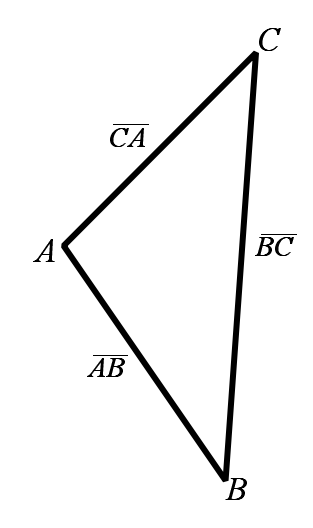
\includegraphics[width=0.2\textwidth]{bilder/dreieck_abc.png}
  \caption[Ein Dreieck als Beispiel für ein Polygon]{\centering Dreick mit Ecken $A, B, C$ als Beispiel für ein Polygon}
  \label{fig:triangle}
\end{wrapfigure}

Dabei ist es wichtig, dass die Anzahl von Strecken endlich ist. "Das Polygon, [zu Deutsch Vieleck], ist also eine durch eine Folge von Strecken begrenzte ebene Fläche." \cite{polydef}
Das einfachste Beispiel hierfür ist ein Dreicke. Es besitzt die Eckpunkte $A$, $B$ und $C$ und wir daher vom Streckenzug aus den Strecken $\overline{AB}$, $\overline{BC}$, $\overline{CA}$ begrenzt (s. Abbildung \ref{fig:triangle}).
Mit genau diesem Prinzip lassen sich beliebig komplexe Polygone erzeugen und beschreiben. Die Strecken werden auch als \textbf{Seiten} und die Endpunkte dieser Strecken 
als \textbf{Ecken} bezeichnet. 
Es sei angemerkt, dass Kreise, obwohl sie ebenfalls ebene Flächen sind, keine Polygone sind. Das folgt daraus, dass Kreise weder Ecken noch eine Begrenzung aus Strecken besitzen.

\subsubsection{Klassifikation von Polygonen}

Es ist denkbar, dass sich die Seiten des Polygons schneiden oder berühren. Man bezeichnet dieses Polygon als überschlagen.\cite{polydef}
Des weiteren kann man Polygone in regulär und nicht regulär unterteilen.
Ein Polygon mit den $n$ Seiten $a,b,c, \ldots$  und den Innenwinkeln $\alpha ,\beta ,\gamma ,\ldots$ heißt regulär, wenn

\begin{center}
  $a=b=c=\dots$ und  $\alpha =\beta =\gamma =\dotsb$
\end{center}
gilt. In einem regelmäßigen Polygon sind demnach alle Seiten zueinander kongruent und alle Winkel gleich groß. \cite{regpoly}

Eine weitere Unterteilungsmöglichkeit lautet wie folgt.
Ein Polygon heißt \textbf{konvex}, wenn für alle Innenwinkel $\alpha _i~(i \in \mathbb{N})$ gilt:
  $\alpha _i < 180^\circ$ 
Anderenfalls heißt es \textbf{konkav}. \cite{convex}

\begin{figure}[t]
  \centering
  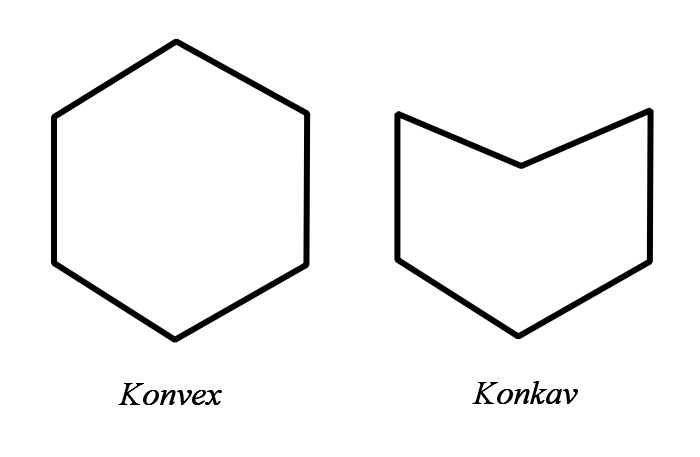
\includegraphics[width=0.5\textwidth]{bilder/konvex_konkav.png}
  \caption[Zwei Secksecke als Beispiel für konvexe bzw. konkave Polygone]{Zwei Secksecke: links konvex, rechts konkav}
  \label{fig:konvexkonkav}
\end{figure}
\pagebreak 
\subsubsection{Diagonalen}

Außer des Streckenzuges, welcher die äußere Grenze des Polygons bildet, kann man im Polygon selbst auch weitere Strecken definieren, 
welche dann als \textbf{Diagonalen} bezeichnet werden. Mittels dieser Diagonalen ist es möglich, jedes Polygon in Dreiecke zu zerlegen. 
Das wird in den nächsten Kapiteln noch näher erläutert, da dieser Sachverhalt die Grundlage für sämtliche Zerlegungsalgorithmen darstellt. 

\subsubsection{Ear und Ear Tips}

Für den in Kapitel 3.3 beschreibenen \ac{eca} ist es der Begriff des \textbf{Ear} (Ohr) relevant. 
Ein Dreieck, welches aus drei aufeinanderfolgenden Ecken $v_{i_0}, v_{i_1}, v_{i_2}$ des Polygons gebildet wird, ohne dass andere Ecken innerhalb 
dieses Dreiecks liegen oder dass der äußere Streckenzug des Polygons durch die Seiten des Dreiecks geschnitten wird, nennt man Ear. Dabei soll die 
Strecke $\left\{v_{i_0}, v_{i_2}\right\}$ eine Diagonale des Polygons. Die Ecke $v_{i_1}$ heißt dann \textbf{Ear Tip}.\cite{meister}

\begin{figure}[h]
  \centering
  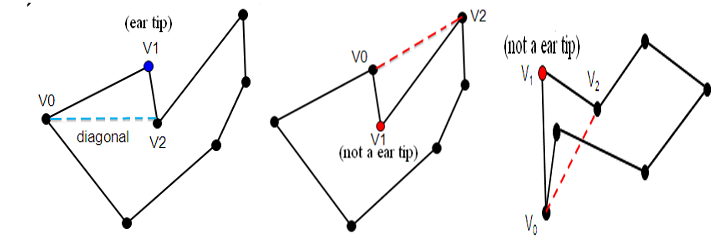
\includegraphics[width=1\textwidth]{bilder/eartips.PNG}
  \caption[Beispiele für Ear und Ear Tips in Polygonen]{\centering Links ist  $\triangle v_{i_0}, v_{i_1}, v_{i_2}$ Ear und $v_{i_1}$ Ear Tip. In der Mitte und rechts 
  ist $\triangle v_{i_0}, v_{i_1}, v_{i_2}$ kein Ear, da $\left\{v_{i_0}, v_{i_2}\right\}$ keine Diagonale ist. \cite{newAlg}}
  \label{fig:ear_eartip}
\end{figure}

\subsubsection{Sätze über Polygone}

Für Polygone gibt es einige Erkenntnisse, welche für die allgemeine Strukturanalyse von eben diesen oder auch für die Triangulation mittels 
\ac{eca} von Bedeutung sind. \break

\begin{flushleft}
  { \textbf{Satz 1 (Jordan'scher Kurvensatz):}

In der euklidischen Ebene $\mathbb{R}^2$ zerlegt jede geschlossene Jordan-Kurve $C \subset \mathbb{R}^2 $ deren Komplement $\mathbb{R}^2 \setminus C$ 
in zwei disjunkte Gebiete, deren gemeinsamer Rand die Jordankurve $C$ ist und deren Vereinigung zusammen mit die ganze Ebene $\mathbb{R}^2$ ausmacht.
\linebreak Genau eines der beiden Gebiete, das sogenannte \textbf{Innengebiet}, ist eine beschränkte Teilmenge von $\mathbb{R}^2$.
\linebreak Das andere dieser beiden Gebiete ist das sogenannte \textbf{Außengebiet} und unbeschränkt. \cite{jordan}
}
\end{flushleft}

\begin{flushleft}
{ \textbf{Satz 2 (Dreieckszerlegung:)}
  
  Jedes Polygon $P$ mit $n$ Ecken kann mittels hinzunahme von null oder mehr Diagonalen vollständig in Dreiecke zerlegt werden. \cite{newAlg}}
\end{flushleft}

\begin{flushleft}
  { \textbf{Satz 3 (Anzahl der Diagonalen:)}
  
  Jede Triangulation eines Polygons $P$ mit $n$ Ecken besteht nutzt $(n-3)$ Diagonalen und besteht aus $(n-2)$ Dreiecken. \cite{newAlg}
}
\end{flushleft}

\begin{flushleft}
  \textbf{Satz 4 (Two Ears Theorem:)}
  
  Jedes Polygon $P$ mit $n \geq 4$ Ecken besitzt mindestens zwei nicht überlappende Ears. \cite{twoears}
\end{flushleft}

\subsubsection{Polytope}
Zuletzt sei an dieser Stelle angemerkt, dass ein Polygon die zweidimensionale Ausprägung des topologischen Begriffs des \textbf{Polytops} ist.
Betrachtet man die räumlichen Dimensionen null bis vier in aufsteigender Reihenfolge so sind ein Punkt, eine Strecke, ein Quadrat, ein Würfel und ein Tesserakt.
Dies ist in der nachstehenden Abbildung zu sehen.

\begin{figure}[h]
  \centering
  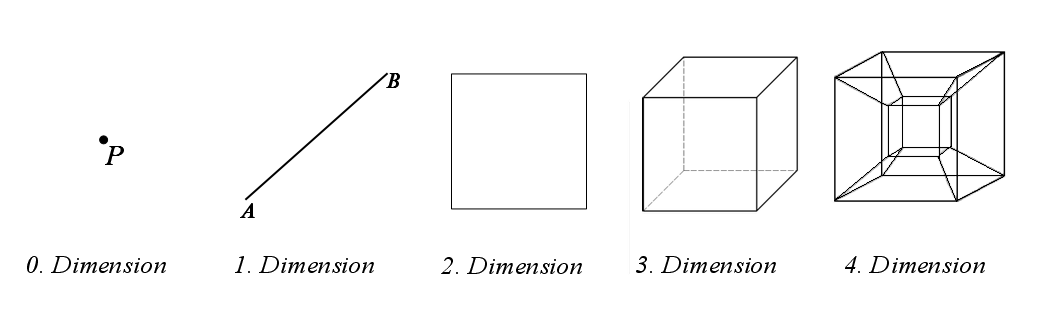
\includegraphics[width=0.9\textwidth]{bilder/Polytope_Dim0_4.png}
  \caption[Beispiele für Polytope der Dimensionen 0 bis 4]{Beispiele für Polytope der Dimensionen 0 bis 4}
  \label{fig:polytope}
\end{figure}

\subsection{Simplexe und Triangulation}

Wie bereits angesprochen kann man durch hinzufügen von Diagonalen in einem Polygon, dieses in Dreiecke oder allgemeiner in Unterpolygone 
zerlegen. Diese Eigenschaft macht sich die \textbf{Triangulation} zu nutze. Allgemein beschreibt der Begriff Triangulation die Zerlegung eines 
topologischen Raumes in \textbf{Simplexe}.\cite{polytri3} Der topologische Raum ist in diesem Fall das Polygon, welches durch einen Streckenzug gebildet wird.

Als Simplex bezeichnet man das einfachste Polygon einer Dimension.\cite{simplex} Für die nullte Dimension ist das trivialer Weise der Punkt. Da keine räumliche Ausdehnung 
möglich ist, ist der begrenzende Streckenzug hier nur der Punkt selbst.
In der ersten Dimension, in welcher Objekte eine Länge aber keine Breite besitzen, ist der Streckenzug eine einzelne Strecke. Diese ist somit auch das Simplex dieser Dimension.
Für die zweite Dimension ist nun das Dreieck das Simplex. Es ist die Fläche, welche aus den wenigsten Punkten, verbunden duch Strecken, erzeugt werden kann und daher das einfachste Polygon dieser 
Dimension. 

Wie bereits beschrieben, kann jedes komplexere Polygon so durch Diagonalen zerlegt werden, dass es volständig von Dreiecken repräsentiert wird. Das ist besonders günstig für 
eine Bearbeitung durch Computer, da ein Dreieck immer eindeutig durch seine drei Eckpunkte beschrieben wird. Diese Form ist daher speichereffizienter als beispielsweise ein allgemeines Viereck, 
für welches nicht nur die Ecken, sondern auch die Kanten gespeichert werden müssten, da mehr als eine Möglichkeit existiert diese vier Punkte zu einem Streckenzug zu verbinden.

Da in der Praxis nicht nur zweidimensionale sondern auch dreidimensionale Objekte eine Rolle spielen, stellt sich die folgende Frage. Kann man diese 3D-Objekte nicht auch in ebenfalls dreidimensionale 
Simplexe zerlegen? 

\begin{wrapfigure}{l}{0.25\textwidth}
  \centering
  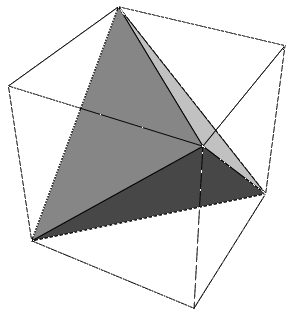
\includegraphics[width=0.2\textwidth]{bilder/cube.png}
  \caption[Zerlegung eines Würfels in vier Tetraeder]{\centering Zerlegung eines Würfels in vier Tetraeder \cite{cubecut}}
  \label{fig:cubecut}
\end{wrapfigure}

Die Antwort ist ja, jedoch ist das nicht sonderlich nützlich. Natürlich existiert in der dritten Dimension auch ein Simplex. Dieses ist der Tetraeder. Man kann auch jedes Polytop 
dieser Dimension in Tetraeder zerlegen, nur benötigt man diese Zerlegung nicht. 
Wöllte man das Innere eines Objektes durch die Zerlegung ebenfalls erhalten, beispielsweise einen Vollwürfel aus Holz in der 
Realität zersägen, dann wäre eine Tetraederzerlegung notwendig. Ein Beispiel für diese Art der Zerlegung ist in Abbildung \ref{fig:cubecut} zu sehen. 
Da man in der digitalen Welt keine echten ausgefüllten Volumina betrachtet sondern nur die Oberfläche darstellt, ist dieses verfahren für die 
Computergrafik uninteressanrt. Man kann die räumlich orientierte Oberfläche eines Würfels topologisch isomorph zu einem Würfelgitter aus quadratischen Flächen beschrieben. Diese Gesamtfläche lässt sich dann 
wiederum in Dreiecke zerlegen. Somit lässt sich auch die Oberfläche dreidimensionaler Objekte durch eine Triangulierung beschreiben. Das ist besonders gut geeigent für Computer, da man nur einen einzigen 
Algorithmus zur Bearbeitung von Flächen und Körpern benötigt, wenn man diese in Dreiecke zerlegen möchte.

\begin{figure}[h]
  \centering
  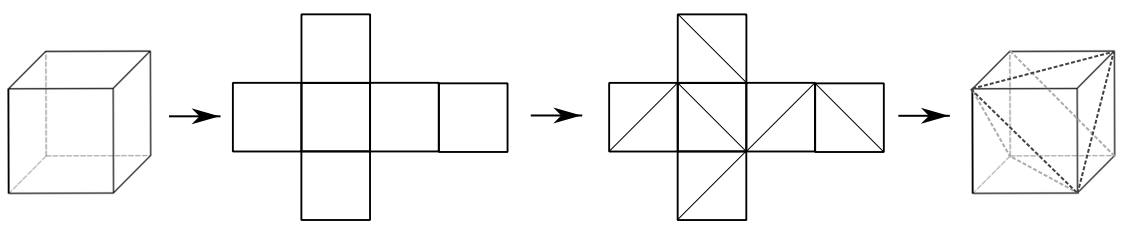
\includegraphics[width=0.9\textwidth]{bilder/3DZerlegung.png}
  \caption[Zerlegung der Oberfläche eines Würfels in Dreiecke mittels Würfelgitter]{\centering Zerlegung der Oberfläche eines Würfels in Dreiecke mittels Würfelgitter}
  \label{fig:cubenet}
\end{figure}

\subsection{Slivers}

Bei Triangulationsalgorithmen wie dem \ac{eca} liegt der Fokus zunächst nicht in der Qualität der Zerlegung. Natürlich gibt es verbesserte Versionen wie beispielsweise in Kapitel 3.1 beschreiben wird.
In jedem Fall sind sogenannte \textbf{Slivers} jedoch ein negativer Einflussfkator, wenn es um qualitative Gesichtspunkte geht. Dreiecke haben in der Computergrfaik die Eigenschaft, dass wenn man eine Scanline 
durch das Dreieck legt, dann schneidet diese ein Dreieck zweimal die Kanten des Dreieck. Diese zwei Schnittpunkte, werden von zwei unterschiedlichen Pixeln auf dem Bildschirm repräsentiert. Somit lässt sich definieren, 
wo eine Fläche beginnt und wo sie endet und dies auf dem Bildschirm darstellen. Bei Slivers ist das nicht der Fall. Ihre Innenfläche ist so schmal,
dass die beiden Schnittpunkte der Scanline mit den Kanten des Dreiecks auf den selben Pixel fallen. \cite{sliverdef} Das führt in letzter Instanz zu Grafikfehlern. 

\begin{wrapfigure}{r}{0.54\textwidth}
  \centering
  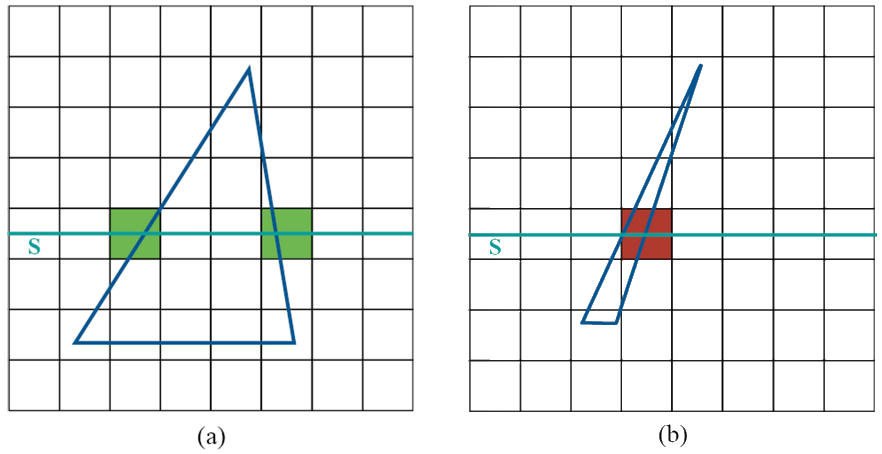
\includegraphics[width=0.49\textwidth]{bilder/sliverScanline.png}
  \caption[Unterschied Sliver und normales Dreieck]{\centering (a) Scanline mit zwei seperaten Schnittpunktpixeln (b) Sliver mit nur einem Pixel für beide Schnittpunkte}
  \label{fig:sliver}
\end{wrapfigure}

Der Begriff Sliver beschränkt sich nicht nur auf Dreiecke. Auch andere Simplexe wie Tetraeder können Simplexe sein. Dass sind diese so flach, dass auch hier Darstellungsfehler entstehen.
Zusätzlich dazu gibt es noch den verwandten Begriff der \textbf{Neadle}, der in Bezug auf Tetraeder, einen sehr schmalen aber auch sehr spitzen solchen bezeichnet.\cite{sliver} \linebreak

\subsection{Der Traditionelle Ear-Clipping-Algorithmus}

Der, in dieser Arbeit, zentrale Punkt, ist der \ac{eca}. Dieser wurde von Meister in seiner Abhandlung \emph{Polygons have ears} \cite{meister} in seiner ursprünglichen Form beschrieben.
Der Algorithmus bestimmt Dreiecke, welche die Eigenschaft eines Ears erfüllen, fügt die dafür nötige Diagonale in eine Liste ein und löscht den Punkt, welcher ein Ear Tip ist aus der Liste aller noch nicht 
bearbeiten Punkte. Dies wird solange wiederholt, bis das Restpolygon nurnoch aus drei Punkten besteht. Zuletzt wird die Lister der Diagonalen ausgegeben, da diese die Triangulation des Polygons erzeugt.
Der Algoritmus ist im Folgenden in Pseudocode dargestellt.

\begin{flushleft}
  { \textbf{Algorithmus 1: Traditionelles Ear-Clipping} \cite{improvedeca}
        \begin{tabbing}
          \=$~~~~~~$\= \textbf{Eingabe:} $~~~$\= Polyg\=on $P$ mit $n$ Ecken in einer Liste $L$\\
          \> \> \textbf{Ausgabe:} \> Liste $D$ mit $n-3$ Diagonalen, die eine Triangulierung bilden.\\
          \> \> \textbf{Schritt 1:} \>Sei $D := \emptyset$ Liste der Diagonalen.\\
          \> \> \textbf{Schritt 2:} \>\textbf{while} $|L| > 3$ \textbf{do}\\
          \> \>                     \> \> (a) Finde ein Ear $v_{i-1}, v_i, v_{i+1}$\\
          \> \>                     \> \> (b) $D := D \cup \left\{v_{i-1} v_{i+1}\right\}$\\
          \> \>                     \> \> (c) $L := L\setminus v_i$\\
          \> \> \> \textbf{endwhile}\\
          \> \> \textbf{Schritt 3:} \> Ausgabe von $D$ als triangulierende Diagonalen.
        \end{tabbing}
}
\end{flushleft}

Dieser Algoritmus hat einen Zeitaufwand von $O(n^3)$ mit einem Aufwand von $O(n^2)$ für das Ermitteln des Ear-Status eines Dreiecks. 
In dieser Formulierung wird nicht auf die Klassifikation eines Ears im speziellen eingegangen. Hierfür beginnt man klassisch 
beim ersten ersten Punkt in $L$. Man überprüft ob dieser Punkt $v_i$ konvex ist. Ist das der Fall, dann muss die Strecke $\left\{v_{i-1}v_{i+1}\right\}$ die Eigenschaft haben, 
eine Diagonale von $P$ zu sein. Wenn das ebenfalls zutrifft, dann ist das Dreicke $v_{i-1}, v_i, v_{i+1}$ ein Ear. 
Man kann die Klassifikation so darstellen:

\begin{flushleft}
  { \textbf{Algorithmus 2: Ear Klassifikation}
        \begin{tabbing}
          \=$~~~~~~$ \= \textbf{Eingabe:} $~~~$\=  Ecken \=${v_i, v_{i-1}, v_{i+1}} \in L$  $~~~~~~~~$\= \\
          \> \> \textbf{Ausgabe:} \> $\triangle v_{i-1}, v_i, v_{i+1}$ ist Ear oder nicht.\\
          \> \> \textbf{Schritt 1:} \>\textbf{if} $v_i$ konvex\\
          \> \> \> \>\textbf{if} $\left\{v_{i-1}v_{i+1}\right\}$ ist Diagonale von $P$\\
          \> \> \> \> \>Ausgabe $\triangle v_{i-1}, v_i, v_{i+1}$ ist Ear.\\
          \> \> \> \> \textbf{else} \>Ausgabe $\triangle v_{i-1}, v_i, v_{i+1}$ ist kein Ear.\\
          \> \> \> \> \textbf{endif}\\
          \> \> \> \textbf{else} Ausgabe $\triangle v_{i-1}, v_i, v_{i+1}$ ist kein Ear.\\
          \> \> \> \textbf{endif}\\
        \end{tabbing}
}
\end{flushleft}
Diese Klassifikation könnte man auch zuerst über alle Punkte $v_i$ in $L$ laufen lassen. Man spricht dann von der Klassifikationsphase. 
Danach kann man in einer zweiten Phase, der Cutting-Phase, Dreicke auswählen, welche die Ear-Eigenschaft erfüllen und sich nicht überschneiden, 
und diese dann Abschneiden. Mit diesen beiden Phasen im Wechsel kann man ebenfalls eine Triangulation erreichen. 
O'Rourke beschreibt in seinem Buch einen Ansatz, der einige Zeitersparnis bei diesem Algorithmus bewirkt.\cite{orourke}
Anstatt nach dem Abtrennen eines Ear Tip Punkts den Status jedes Eckpunktes erneut zu überprüfen, muss man nur den Status von $v_{i-1}$ und $v_{i+1}$ erneut betrachten.
Nur diese beiden Punkte sind nämlich vom Abtrennen von $v_i$ beeinflusst. Somit benötigt man insgesamt nurnoch eine Zeit von $O(n^2)$.\cite{newAlg} 
In jedem Cutting-Schritt kann man dann zusätzlich entscheiden, welche Dreieck als nächstes ausgewählt werden soll. So könnte an nur die Dreiecke auswählen, welche einer bestimmten Heuristik entsprechen.
Beispielsweise könnten so nur Dreiecke gewählt werden, bei denen der kleinste Innenwinkel das Maximum aller aktuell verfügbaren Innenwinkel ist. Auf diese Weise ist es denkbar,
dass man Sliver vermeiden könnte. Andere Ansätze sind exemplarisch im folgenden Abschnitt aufgeführt.
\section{Verwandte Arbeiten}
\subsection{Verbesserungen des Ear-Clipping-Algorithmus}

Wenn man einen Algorithmus mathematisch betrachtet, dann ist die Zeit, welcher er bis zur Terminierung benötigt, zumeist der
Gegenstand der Betrachtung. Mittels der Komplexitätstheorie lässt sich eine vom Computertyp unabhängige Beschreibung dafür finden. 
Das Referenzmodell ist dabei zumeist die \ac{tm}.\cite{tm} Ziel ist es, dass ein Algorithmus 
auf einer \ac{tm} in Polynomialzeit abläuft. Diese Zeit hängt zumeist von der Eingabegröße ab. Für den \ac{eca} ist die entscheidende 
Größe die Anzahl der Ecken $n$ des Polygons $P$.
Betrachtet man den \ac{eca} auf einer \ac{tm}, so hat er eine Komplexität von $O(n^3)$.
Zwar ist dieser Term ein Polynom in $n$, jedoch ist das kein Grund für die Wissenschaft, hier mit der Optimierung aufzuhören.
Wie O'Rourke in seiner Arbeit zeigt, kann man den \ac{eca} durch kleine Änderungen so modifizieren, dass dieser eine Komplexität von $O(n^2)$
aufweist.\cite{orourke} Diese Erkenntnis nutzen Mei, Tipper und Xu, um den Algorithmus auf andere Art zu verbessern.\cite{earclipping}

Für einen Algorithmus wie den \ac{eca} ist nicht nur seine Laufzeit entscheidend. Während andere Algorithmen beispielsweise Entscheidungsprobleme lösen, 
bei denen es nur um die Frage nahc der Existenz der Lösung geht, ist bei einer Triangulation bereits bekannt, dass es unterschiedliche Lösungen gibt.
Daher ist die Frage nicht, ob eine Lösung existiert, sondern ob eine optimale solche gefunden werden kann. Optimal ist dabei ein relativer Begriff, 
der stark von den Rahmenbedingungen abhängt. Für den \ac{eca} ist der Speicherbedarf ebenfalls entscheidend. Dieser ist bei Mei, Tipper und Xu durch $O(n)$
begenzt. Das Ziel ihrer Arbeit war es, qualitytiv hochwertige Triangulationen für komplexe Polygone zu erzeugen. Der Qualitätsparameter war dabei der kleinste 
Innenwinkel der erzeugten Dreiecke in der Zerlegung. Genauer ging es darum, die sogenannten Slivers zu vermeiden (s. Kapitel 2.3).

Ihr Ansatz war es, den verbesserten Algorithmus von O'Rourke so zu modifizieren, dass er über die Option des \textbf{Edge Swappings} verfügt.
Wird ein Ear erkannt, dann wird für jeden seiner Innenwinkel überprüft, ob dieser kleiner ist als ein zuvor festgelegter Grenzwert. Ist das der Fall, dann 
muss bei diesem Dreieck Edge Swapping durchgeführt werden. Dafür werden der größte Innenwinkel des Dreiecks und die, ihm gegenüberliedende, längste Seite bestimmt.
Daraufhin wird überprüft, ob es ein Nachbardreieck gibt, welches sich mit dem Ursprünglichen eben diese längste Seite teilt. Gibt es einen solchen Nachbarn, 
dann wird in dem von den beiden Dreiecken gebildeten Viereck eine Diagonale zwischen den beiden Ecken gezogen, welche jeweils der zuvor bestimmten längsten Seite gegenüber lagen.
Auf diese Art entstehen wieder zwei Dreiecke, von denen nun die Innenwinkel auf ihre Größe überprüft werden. Ist jeweil der kleinste Winkel größer als der Grenzwert, 
dann ist die Qualität der Dreiecke nun besser als die des ursprünglich Ausgewählten. Wenn dem nicht so ist, bleibt alles unverändert und das Ear wird wie es war gewählt und abgeschnitten.

%Grid Impementierung FIST
% Im FIST-Paper wird noch auf eine weitere wichtige Verbesserungstechnik eingegangen: Spatial-Hashing-Verfahren (z.B. Grids), um die Menge der Vertices einzuschränken, 
% die pro potentiellem Ear getestet werden. Kannst Du darauf evtl. noch eingehen? So ein Grid ist auch in meiner Rust-Implementierung enthalten.

\begin{figure}
    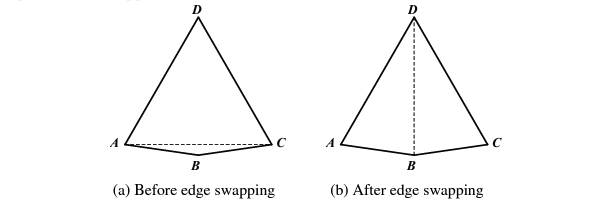
\includegraphics[width=1\textwidth]{bilder/edgeswapping.png}
    \caption[Edge Swapping]{Edge Swapping \cite{earclipping}}
    \label{fig:edgeswapping}
\end{figure}

Auf diese Art kann die Qualität der Dreiecke in der Triangulation stark erhöht werden. Sie zeigen an Beispielen, dass sich die Innenwinkelgröße durchschnittlich verdoppelt.
Teilweise können Dreiecke mit minimalem Innenwinkel von $< 15^\circ$ ganz eliminiert werden. Das hängt jedoch vom eingegebenen Poylgon ab und hat keine Allgemeingültigkeit.

\subsection{Parallelisierung des Ear-Clipping-Algorithmus}

Anstatt den Algorithmus selbst in seiner Laufzeit zu verbessern, ist es ein Gedanke, die Abarbeitung aufzuteilen. Vorallem mit der technischen Entwicklung mehrerer Prozessorkerne in einer \ac{cpu}
ist verteiltes Rechnen ein gängiges Konzept. Hierzu haben Eder, Held und Palfrader eine Arbeit verfasst, die sich mit der Umsetzung des \ac{eca} unter dem Gesichtspunkt der coarse-grain parallelization,
zu Deutsch grobkörnigen Parallelisierung, befasst.\cite{paralleleca} Dieses Prinzip beschreibt die Aufteilung eines Programms in längere Unteraufgaben. Das ist ein für Multicore Computer sehr geeignetes Konzept.
Andere Arbeiten befassten sich auch mit der Umsetzung der Arbeitsteilung, aber dort speziell mit dem Konzept der fine-grain parallelization im Bezug auf die \ac{dt}. Die fine-grain parallelization, also die feinkörnige 
Parallelisierung, beschreibt die Aufteilung eines Programms in eine Vielzahl kleinerer Aufgaben. 
Hier ist beispielsweise M. Goodrich\cite{goodrich} zu nennen.

Eder, Held und Palfrader haben ihre Arbeit auf \ac{fist} aufgebaut. Dieses Framework ist ein in C++ verfasster Code für Polygontriangulation basierend auf dem \ac{eca}.\cite{paralleleca}
Sie beschränkten sich dabei mit der Parallelisierung auf den Bereich des Algorithmus, welcher sich mit der Klassifikation und dem Clipping der Ears befasst. Dieser Teil macht etwa $80\%$ des Rechenaufwandes aus.
Um eine Aufteilung in $k$ Threads zu erreichen, welche dann auf den $k$ Kernen der \ac{cpu} abgearbeitet werden sollen, nutzen Sie drei verschiedene Ansätze und vergleichen diese miteinander und mit der nicht parallel 
laufenden Form des Algorithmus in \ac{fist}.

Ihr erster Ansatz beruht auf dem \emph{divide-and-conquer-Prinzip}. Anstatt das Polygon $P$ allerding durch Diagonalen in etwa gleich große Unterpolygone $P_k$ zu unterteilen, 
nutzen Sie $k-1$ viele senkrechte Geraden dafür. Dies ist weit weniger aufwendig in der Berechnung, da das Finden von geeigneten Diagonalen relativ rechenintensiv ist.
Sie berufen sich dabei auf einen Algorithmus von Sutherland und Hodgman \cite{dnc}. Bei dieser Form der Unterteilung enstehen sogenannte \ac{sp}, welche die Schnittpunkte der senkrechten Geraden mit 
den Strecken der äußeren Begrenzung darstellen. Dafür benötigt man eine Zeit von $O(n)$ pro Gerade $l$ und fügt im schlimmsten Fall $O(n)$ \ac{sp} ein. Diese werden als neue Eckpunkte in den Unterpolygonen eingefügt und damit vom \ac{eca} auch als Eckpunkte der Dreiecke in der Zerlegung benutzt. 
Das führt dazu, dass Dreiecke in der Gesamtzerlegung von $P$ entstehen, welche unzulässige Eckpunkte besitzen, da diese im Ursprünglichen Polygon nicht existieren. 
Dafür muss eine Bereinigung der Zerlegung durchgeführt werden, nachdem alle $k$ Threads ihre Triangulation der $P_k$ Unterpolygone geliefert haben. 
Durch den Schnitt des Poylgons mit einer senkrechten Geraden entstehen zwei \ac{sp} $s_a$ und $s_b$. Um diese wieder zu löschen, werden alle Dreiecke, welche zu einem dieser beiden Punkte inzident sind, aus der Triangulation 
gelöscht. Auf diese Weise erzeugt man ein Loch $H$ in der Zerlegung, welches wieder ein Polygon ist. Diese kann man nun durch erneute Triangulation mit validen Dreiecken füllen. \linebreak 

Einen \emph{partition-and-cut-Ansatz} zu verwenden, war die zweite Variante, um die Triangulation auf die $k$ Threads aufzuteilen. Dabei wird nicht wie bei \emph{divide-and-conquer} das gesamte Polygon $P$, sondern nur sein begrenzender Streckenzug unterteilt.
Hierfür werden \textbf{Landmarks}, also Wegpunkte, eingeführt. Dies geschieht anhand der Indizierung der $n$ Ecken. Die Eckpunkte mit den Indizes $\left\{ 0, \frac{n}{k}, \frac{2n}{k}, \dots, \frac{(k-1)n}{k} \right\}$ werden die Landmarks. Der Streckenzug zwischen je zwei dieser Markierungen wird 
jeweils einem Thread zugewiesen. Die Wegpunkte gehören dabei jeweils zu zwei benachtbarten Teilstreckenzügen gleichzeitig. Jeder Thread durchläuft dann eine Klassifikations- und eine Clippingphase, bei denen darauf geachtet wird, dass die Landmarks nicht gelöscht werden.
Ist das geschehen und alle Threads beendet, dann bleibt ein Teil des Polygons noch unbearbeitet. Dieser Teil wird bei Eder, Held und Palfrader nicht nocheinaml in Abschnitte für verschiedene Threads unterteilt sondern wird dann vom sequentiellen \ac{eca} in \ac{fist} bearbeitet.
Zwischen den Threads wird keine Synchronisation benötigt, da sowohl Klassifikation als auch Clipping völlig undabhängig von anderen Threads ablaufen und nur in ihrem jeweiligen Abschnitt Dreiecke erzeugt werden. Dabei sei angemerkt, dass das Überprpüfen der Ear-Eigenschaft nur Lesezugriff auf 
die Globale Liste aller Eckpunkte des Polygons benötigt. Der Vorgang der Aufteilung in Threads und deren bearbeitung ist in der nachstehenden Abbildung zu sehen. \linebreak
\begin{figure}[h]
    \centering
    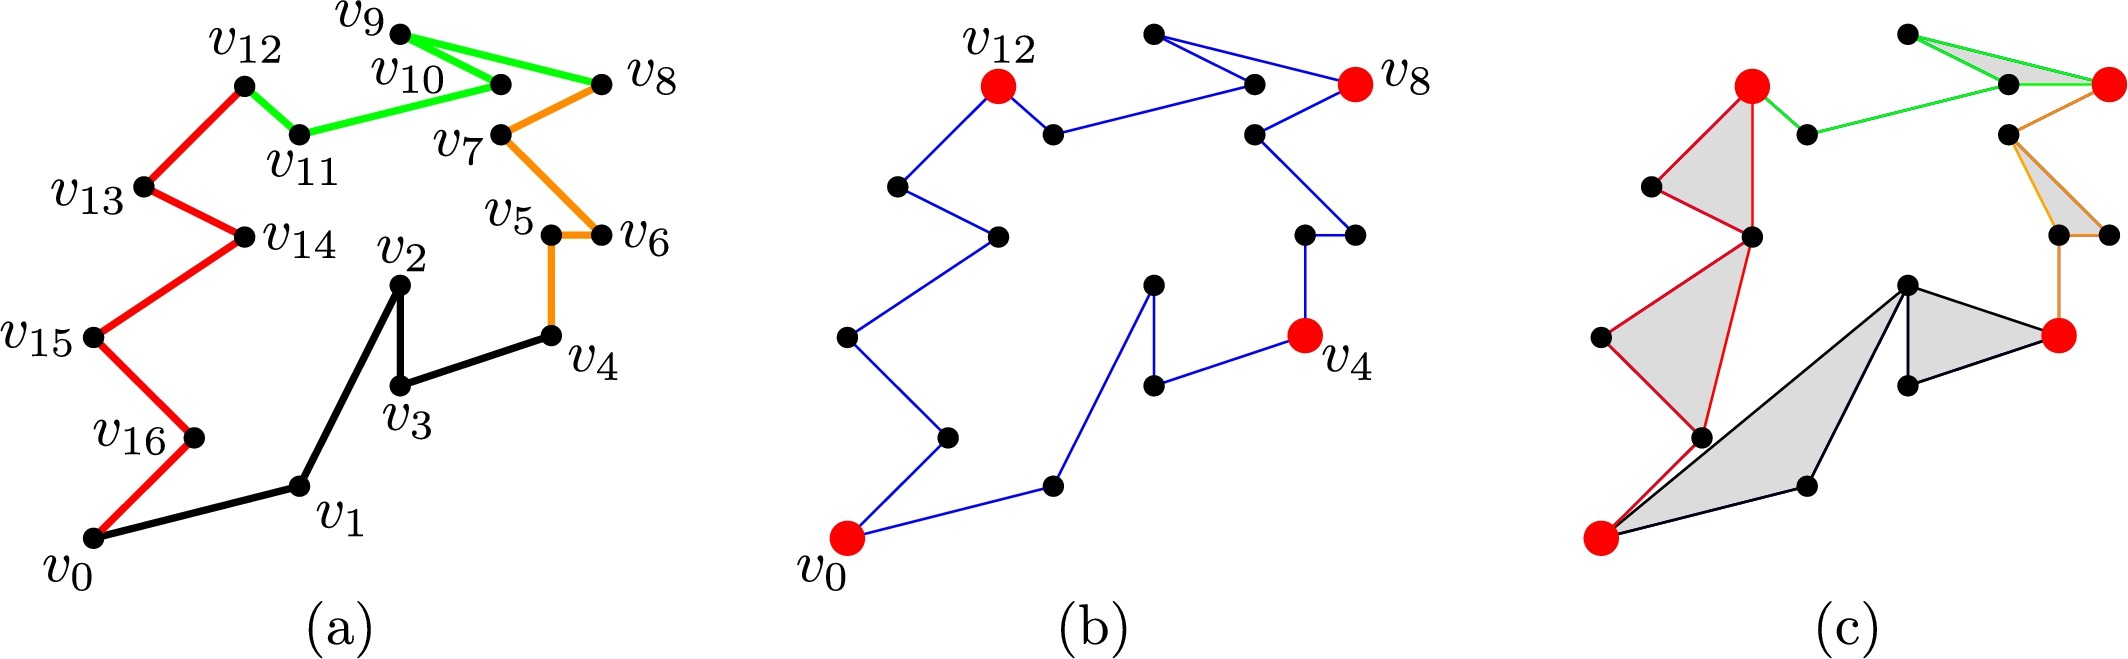
\includegraphics[width=0.8\textwidth]{bilder/segmentierung.jpg}
    \caption[Unterteilung des Streckenzugs in Unterstreckenzüge mittels Landmarks für Parallelisierung]{\centering (a) Einfaches Polygon $P$ unterteilt in vier Streckenzüge (b) Landmarks vervorgehoben (c) Triangulierung durch Threads}
    \label{fig:langmarks}
\end{figure}

Der dritte Ansatz, betreffend dem \ac{eca} in \ac{fist} ist der sogenannte \emph{mark-and-cut-Ansatz}, welcher Ähnlichkeiten zum vorher erwähnten \emph{partition-and-cut-Ansatz} aufweist. Auch in diesem Fall werden einige Eckpunkte von $P$ als Markierungen genutzt.
In der Marierungsphase, durchläuft ein Thread den Streckenzug von $P$ und speichert jeden zweiten konvexen Eckpunkt in einer Liste. Hat dieser Thread die Hälfte aller Punkte überprüft, werden die Cut-Threads gestartet, welche nur die Cutting-Phase durchlaufen. Bildet 
ein Punkt in der Liste mit seiner gegenüberliegenden Seite ein Dreiecke, dann wird dieses sofort als valide gespeichert und abgeschnitten. Jeder dieser Punkte darf nur einmal bearbeitet werden, damit es nicht zu Asynchronität und Redundanz kommt. Wenn die Cut-Threads alle ihre Arbeit getan haben, 
werden sie neu gestartet und bearbeiten dann alle Punkte, die Seit ihrem letzten Start zur Liste hinzugefügt worden sind.
Während dessen durchläuft der Mark-Thread das Polygon erneut und fürgt neue konvexe Punkte zu Liste hinzu und so weiter, bis nurnoch weniger Dreiecke erkannt werden, als vorher mit einem Grenzwert festgelegt. Dieser lag bei Eder, Held und Palfrader bei 20 Dreiecken.
Der Rest von $P$, welcher noch nicht bearbeitet wurde, wird dann wie im \emph{partition-and-cut-Ansatz} von einem sequentiellen Aufruf von \ac{fist} bearbeitet. 

\begin{figure}[b]
    \centering
    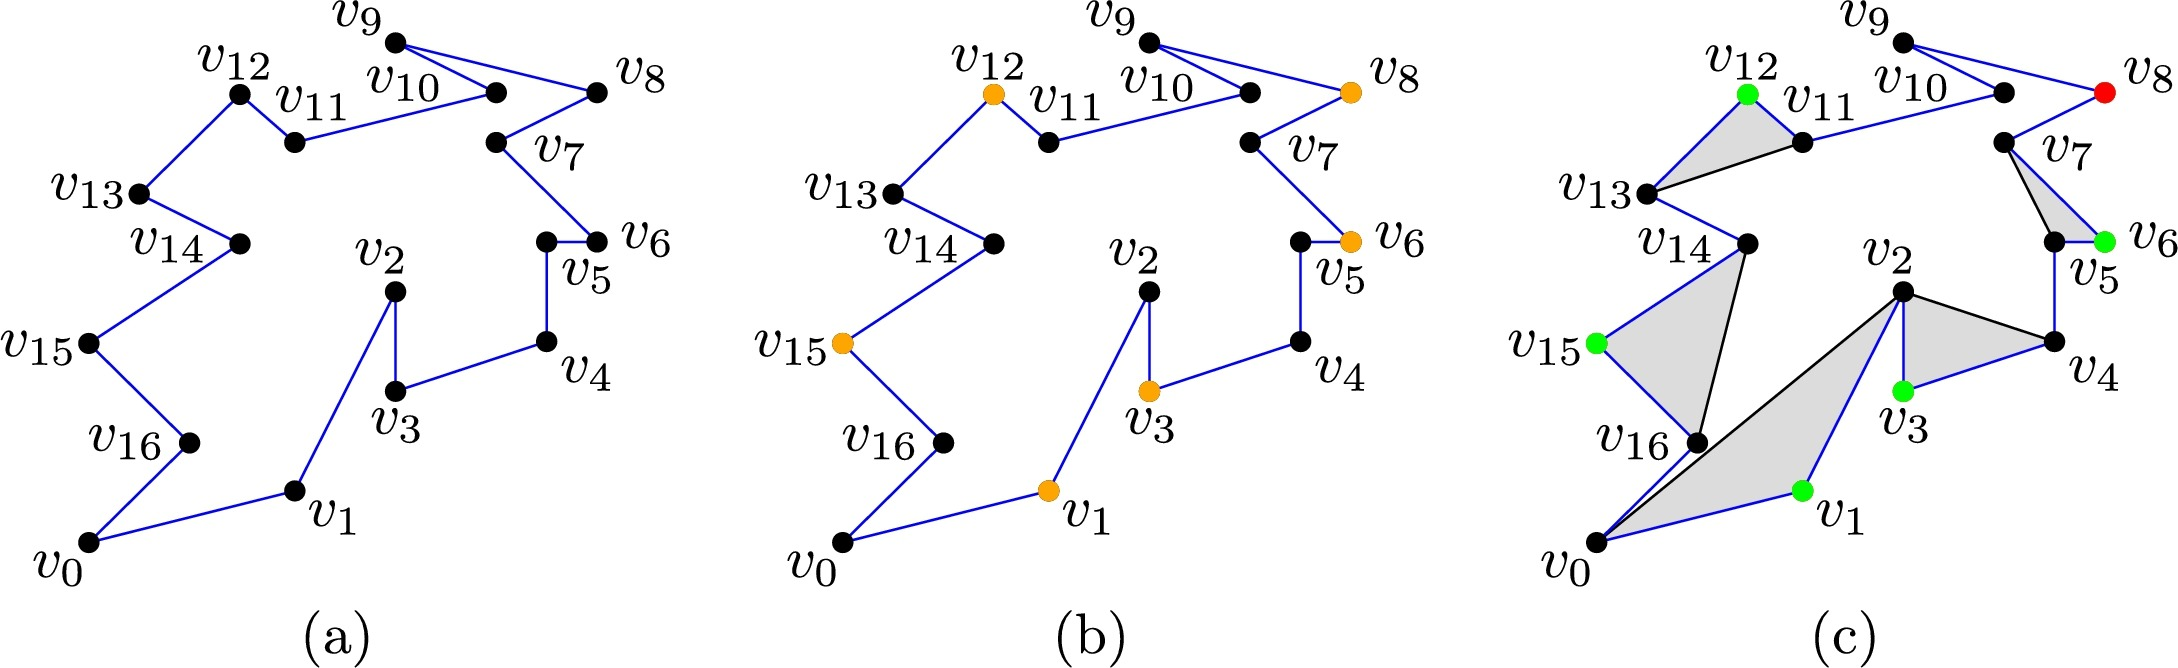
\includegraphics[width=0.8\textwidth]{bilder/markierung.jpg}
    \caption[Markierung konvexer Eckpunkte für Parallelisierung]{\centering (a) Einfaches Polygon $P$ (b) Erste Markierungsphase, ausgewählte Ecken in orange (c) Erste Cutting-Phase}
    \label{fig:konvPoints}
\end{figure}

Der finale Vergleich aller drei Ansätze hinsichtlich ihrer Qualität zeigt, dass sie in etwa gleich gut sind. Als Vergleich wurde von ihnen noch eine Variante der \ac{dt}, die sogenannte \ac{cdt} durchgeführt, auf die an dieser Stelle allerdings nicht 
genauer eingegangen werden soll. Die folgende Tabelle zeigt das Ergebnis.

\begin{table}[h]
    \begin{tabular}[h]{| l | c | c | c | c | c |}
    \hline
    & CDT & FIST's top & D\&C & P$\&$C & M$\&$C \\ \hline
    (1) Durchschn. Abw. 60° & 30.79° & 31.53° & 35.29° & 34.97° & 38.38° \\ \hline
    (2) Durchschn. min. Winkel & 24.60° & 23.40° & 20.07° & 21.32° & 21.07° \\ \hline
    \end{tabular}
    \caption[Vergleich verschiedener Parallelisierungen des \ac{eca} in \ac{fist}]{Vergleich der \ac{fist} Trianulation inklusive \ac{cdt} und FIST's top Heuristik. Aufgeführt sind folgende Parallele Versionen von \ac{fist}: 
    Divide-and-conquer D\&C, Partition-and-cut P\&C und Mark-and-Cut M\&C. 
    (1) Durchschnittliche Abweichung aller Innenwinkel von 60° über alle Triangulationen (je kleiner, desdo besser) 
    (2) Durchschnittliche Größe des kleinsten Innenwinkels aller Dreiecke über alle Trinagulationen (je größer, desdo besser) \cite{paralleleca}}
    \label{tab:tab1}
\end{table}

\subsection{Alternative Verfahren und Ansätze} 

\subsubsection{Delauny Triangulation}

Spricht man von Triangulationen, so stößt man zwangsläufig auf den Begriff der Delauny Triangulation. Sie ist, qualitativ gesehen, die Triangulation mit den ausgewogensten Dreiecken.

\begin{wrapfigure}{lh}{0.25\textwidth}
    \centering
    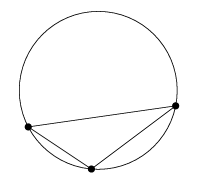
\includegraphics[width=0.23\textwidth]{bilder/umkreis.png}
    \caption[Umkreis eines Dreiecks]{\centering Umkreis eines Dreiecks \cite{delauny}}
    \label{fig:umkreis}
  \end{wrapfigure}

Um jedoch zu verstehen wie die \ac{dt} gebildet wird, benötigt man den Begriff des \emph{leeren Umkreises}. Sie ist die grundlegende Bedingung für eine \ac{dt}, da man nur solche Triangulationen, in denen alle Dreiecke eben diese 
Bedingung des leeren Umkreises erfüllen, eine \ac{dt} nennt.\cite{delauny}

Man betrachte eine Menge aus Punkten $V$ in der euklidischen Ebene $\mathbb{R}^2$. Ein Dreieck $\triangle v_1v_2v_3$ mit $v_1, v_2, v_3 \in V$ erfüllt die Bedingung des leeren Umkreises, wenn der Kreis, welcher durch die drei Punkte $v_1, v_2, v_3$ geht, 
keine anderen Punkte $v_i \in V$ beinhaltet. 

Kann man also eine Menge aus Dreiecken $T$ finden, sodass jeder Punkt der Menge $V$ teil mindestens eines Dreiecks ist und jedes Dreieck wenigstens eine Seite mit einem anderen Dreieck teilt, dann
ist die $T$ eine \ac{dt} von $V$, wenn jedes Dreieck in $T$ einen leeren Umkreis besitzt. 

Dass diese Triangulation nicht eindeutig ist, kann mann an einem einfachen Beispiel zeigen. Hat man vier Punkte im $\mathbb{R}^2$, welche alle zueinander konvex sind, dann ist es möglich, dass alle diese Punkte auf dem selben Umkreis liegen.
In einem solchen Fall sind alle möglichen Kombinationen aus sich nicht gegenseitig schneidenden Dreiecken als \ac{dt} zulässig. Jedoch gibt es auch den Fall, dass nur je drei Punkte auf einem Kreis liegen. Dafür gibt es immer zwei Möglichkeiten, von denen 
meist nur eine eine \ac{dt} ist. In Abbildung \ref{fig:fourpointdt} ist sind in den Fällen (a) und (b) diese Möglichkeiten für Umkreise zu sehen, welche einmal eine \ac{dt} erzeugen und einmal nicht. In Fall (c) ist der zuvor beschriebene Fall aufgeführt, 
bei dem die vier Punkte alle auf dem selben Kreis liegen.

\begin{figure}[h]
    \centering
    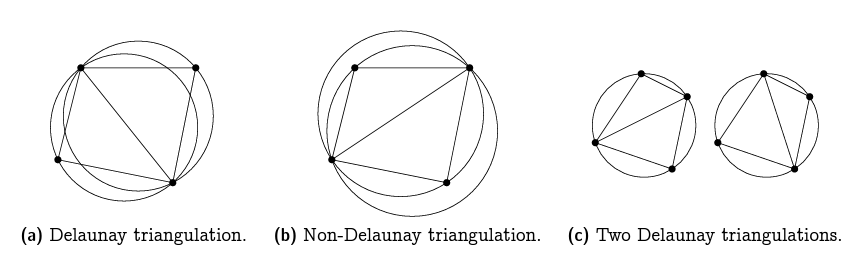
\includegraphics[width=1\textwidth]{bilder/fourpointdt.png}
    \caption[Delauny Triangulation für vier konvexe Punkte]{Delauny Triangulation für vier konvexe Punkte. (a) Delauny Triangulation (b) keine Delauny Triangulation (c) mehrere gleichwertige Triangulationen \cite{delauny}}
    \label{fig:fourpointdt}
\end{figure}

Eine sehr vorteilhafte Eigenschaft der \ac{dt}, welche diese für praktische Anwendungen sehr interessant macht, ist, dass sie den minimalen Innenwinkel jedes Dreiecks der Triangulation maximiert. Das bedeutet, dass die \ac{dt} die qualitativ hochwertigste aller möglichen Triangulationen
einer Menge von Punkten ist. Aber auch so ist es nicht möglich, dass jede \ac{dt} die Bedingung erfüllt, keine Slivers zu enthalten. Es bedeutet lediglich, dass, wenn ein Sliver teil einer \ac{dt} ist, dann wäre auch in jeder anderen Triangulation mindestens ein Sliver enthalten.
Das ist immerhin in sofern eine gute Eigenschaft, da eine \ac{dt} einer Punktmenge immer die minimale Anzahl an Slivers enthält. Sie dient damit als optimaler Vergleich für beispielsweise den \ac{eca}, da man damit die Abweichung der Triangulation des \ac{eca} zu der durch die \ac{dt} erzeugten bestimmen kann. 

\begin{wrapfigure}{hr}{0.35\textwidth}
    \centering
    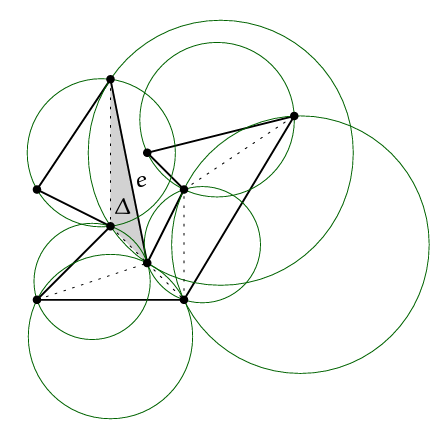
\includegraphics[width=0.35\textwidth]{bilder/cdt.png}
    \caption[Constrained Delauny Triangulation für ein Polygon]{Constrained Delauny Triangulation eines Polygons\cite{delauny}}
    \label{fig:cdt}
\end{wrapfigure}
Möchte man, wie in dieser Arbeit, ein Polygon in Dreiecke zerlegen, so stößt man auf ein Problem. Ein Polygon in zwar eine Menge aus Punkten, jedoch sind diese bereits durch einen Streckenzug fest miteinander verbunden. Man kann in dem meisten Fällen also keine echte \ac{dt} erzeugen, 
da die Dreiecke nicht frei wählbar sind. Man spricht dann von der sogenannten \ac{cdt}. Diese versucht ebenfalls die Bedingung des leeren Umkreises zu erfüllen, allerdings mit einer Einschränkung, welche sie für vorgegebene Polygone umsetzbar macht.
Der Umkreis eines Dreiecks $\triangle$ darf andere Punkte des Polygons enthalten, wenn diese von innerhalb von $\triangle$ nicht sichtbar sind. Ein Punkt $p$ heißt \textbf{sichtbar}, wenn eine Punkt $q$ im Inneren des Dreiecks $\triangle$ existiert, so dass die Strecke $\overline{pq}$ keine andere Strecke $e \in E$ schneidet.
Anderenfalls blockiert $e$ sozusagen die Sicht auf den Punkt $p$.


\subsubsection{Algorithmus basierend auf Sichtbarkeit}

Wie schon bei der \ac{dt} ist hier der Begriff der Sichtbarkeit von Eckpunkten entscheidend. Anders als zuvor werden hier jedoch keine Dreiecke ermittelt,
welche die Bedingung des leeren Umkreises erfüllen. In diesem Algorithmus, beschrieben von Ran Liu, wird das Polygon $P$ in zwei Unterpolygone $P_1$ und $P_2$ unterteilt,
welche dann solange rekursiv weiter unterteilt werden, bis die entstandenen Unterpolygone $P_i$ Dreiecke sind.\cite{newAlg}
Hierfür muss in einem ersten Schritt die Sichtbarkeit jedes Punkte gegenüber einem Referenzpunkt $v_i$ überprüft werden. Dazu betrachtet man zunächst die Nachbarn $v_{i-1}$ und $v_i+1$ 
von $v_i$. Diese begrenzen das sogenannte \textbf{Sichtfeld} von $v_i$, welches mit $\alpha$ bezeichnet wird und dem Winkel in $v_i$ entspricht. Für spätere Betrachtungen zählen $v_{i-1}$ und $v_{i+1}$ 
als nicht sichtbar im BEzug auf $v_i$. Entlang der Kanten von $P$ wird nun ausgehend von $v_{i+1}$ entgegen dem Uhrzeigersinn überprüft, ob ein Punkt $v_j$ im Sichtfeld von $v_i$ liegt.
Ist das der Fall, dann gilt der Punkt $v_j$ als sichtbar, wenn die Strecke $v_iv_j$ eine Diagonale von $P$ ist. Zusätzlich begrenzt dieser Punkt nun das Sichtfeld und es muss verkleinert werden. Das neue Sichtfeld $\alpha$ berchnet sich also durch $\alpha = v_{i-1},v_i,v_j$.
Der Vorgang wird fortgesetzt, bis alle Punkte überprüft sind. Ist diese Überprüfung für alle $v_i$ von $P$ abgeschlossen, wird die Anzahl der sichtaberen Punkte 
gegenüber dem jeweiligen Referenzpunkt bestimmt. Diese dient als Vergleichskriterum für die Punkte untereinander. Als Beispiel ist in der nachfolgenden Abbildung einmal die Ermittlung von $alpha$ und die Überprüfung 
mehrerer Punkte bezogen auf den Punkt $v_0$ dargestellt. 

\begin{figure}[h]
\centering
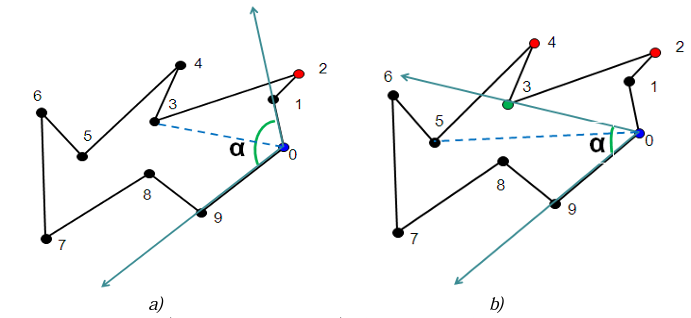
\includegraphics[width=1\textwidth]{bilder/sichtbarkeit.png}
\caption[Sichtbarkeit von Punkten]{\centering(a) $v_3$ ist sichtbar für $v_0$ (b) Überprüfung der Sichtbarkeit von $v_5$ mit neuem Sichtfeld $\alpha$ (nicht sichtbar entspricht rot, sichtbar entspricht grün) \cite{newAlg} }
\label{fig:visibPoint}
\end{figure}

Für die Anzahl sichtbarer Punkte bezogen auf $v_i$ wird die hier Bezeichnung $s(v_i)$ verwendet. Man kann diesen Vorgang der Sichtbarkeitsanalyse wie folgt in Pseudocode beschreiben.

\begin{flushleft}
    { \textbf{Algorithmus 4: Sichtbarkeitsanalyse für einen Punkt $v_i$}
          \begin{tabbing}
            \=$~~~~~~$ \= \textbf{Eingabe:} $~~~$\=  Eck\=en $v_i$\=$ \in V$\=$(P),~n = |V(P)| - 3,~s(v_i)=0$\\
            \> \> \textbf{Ausgabe:} \> Anzahl sichtbarer Punkte $s(v_i)$\\
            \> \> \textbf{Schritt 1:} \> Wähle Referenzpunkt $v_i$ \\
            \> \> \textbf{Schritt 2:} \>$\alpha = \angle v_{i-1}v_iv_{i+1}$\\
            \> \> \textbf{Schritt 3:} \>\textbf{while} $n > 0$ \textbf{do}\\
            \> \> \> \> \textbf{if} $\angle v_{i-1}v_iv_j > 0 \wedge \angle v_{i-1}v_iv_j < \alpha$\\
            \> \> \> \> \> \textbf{if} $v_iv_j$ Diagonale von $P$\\
            \> \> \> \> \> \> (a) $s(v_i)= s(v_i)+1$\\
            \> \> \> \> \> \> (b) $\alpha = \angle v_{i-1}v_iv_j$\\
            \> \> \> \> \> \> (c) $n = n-1$\\
            \> \> \textbf{Schritt 4:} \> Ausgabe von $s(v_i)$ 

          \end{tabbing}
  }
  \end{flushleft}

Ist $s(v_i)$ für jeden Eckpunkt $v_i$ von $P$ ermittelt, wird der Punkt mit der größten solchen Anzhal ausgewählt. Gibt es mehrere solche Punkte, dann 
kann ein beliebige dieser Punkte gewählt werden. Dieser Punkt wird dann als \textbf{First Head} bezeichnet.
Als nächstes wird noch der Punkt mit der zweit höchsten Anzahl $s(v_i)$ gewählt. Er wird als \textbf{Second Head} bezeichnet. Sollte es hier Uneindeutigkeiten
bei der Auswahl geben, dann wird ein Test durchgeführt, um diesen Punkt auszuwählen. Durch die Diagonale zwischen First und Second Head soll das Polygon in zwei 
Unterpolygone zerlegt werden. Man testet, bei welchem der möglichen Punkte für den Second Head, der Betrag der Differenz zwischen der Anzahl an Strecken in den beiden 
Unterpolygonen $P_1$ und $P_2$ am geringsten ist. Das ist in der nächsten Abbildung zu sehen.

\begin{figure}[h]
    \centering
    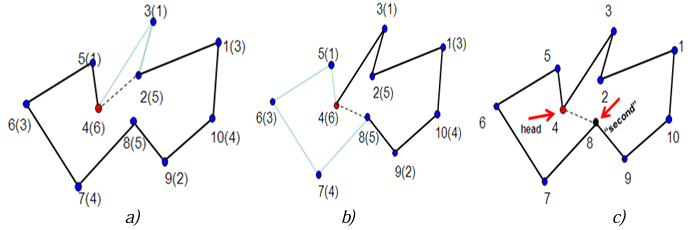
\includegraphics[width=1\textwidth]{bilder/second_head_comp.png}
    \caption[Test zur Auswahl des Second Head]{\centering(a) und (b) Vergleich der Differenz zwischen der Länge des schwazen und des türkiesen Strecknabschnitts (c) Auswahl des Second Head \cite{newAlg} }
    \label{fig:secHead}
\end{figure}

Für die Zerlegung werden First und Second Head dann dupliziert, damit beide Polygone vollständig begrenzt sind. In beiden Unterpolygonen muss dann die Sichtbarkeitsanalyse erneut durchgeführt werden.
Damit dies ein wenig schneller geschieht, kann man die sichtbaren Punkte im Bezug auf einen Punkt $v_i$ in einer sogennanten \emph{single circular list} gespeichert werden. In einer solchen Liste zeigt der Pointer des 
letzten Elements auf das erste Element der Liste. Beim Update der Sichtbarkeiten müssen dann für jeden Punkt nur die Punkte in seiner jeweiligen Liste überprüft werden und jetzt nicht mehr sichtbare Punkte aus der Liste 
gelöscht werden. Damit wird die Laufzeit der Sichtbarkeitsanalyse von $O(n^2)$ auf $O(n)$ begrenzt. Nichtsdesdotrotz hat der neue Algorithmus von Ran Liu, nach seiner eigenen groben Analyse, eine Komplexität von über $O(n^3)$.
Im Vergleich mit dem \ac{eca}, welcher eine Komplexität von $O(n^2)$ besitzt, schneidet er damit schlechter ab. In Tabelle \ref{tab:tab2} und \ref{tab:tab3} werden zwei Beispiele des Vergleichs zwischen dem Sichtbarkeitsalgorithmus 
und dem \ac{eca} aus der Arbeit von Liu angeführt. Die Algorithmen wurden auf zufällig generierten Polygone unterschiedlicher Knotenanzahl und Form getestet. Dabei waren die getesteten Polygonformen einmal \emph{rund}, das heißt 
die Eckpunkte konnten nur in einem quadratischen Koordinatenbereich liegen. Der andere Typ war \emph{länglich}, wobei die Punkte eher in ihrer x-Koordinate weiter streuten, nicht so sehr jedoch in der y-Koordinate.
Es ist in den Ergebnissen dieser Tests ersichtlich, dass die Qualität der Dreiecke bezogen auf ihre minimalen Innenwinkel bei Liu's Algorithmus besser ist, als die des \ac{eca}. In Sachen Laufzeit jedoch schneitet der neue Algorithmus jedoch schlechter ab,
wie bereits die Komplexitätsanalyse zeigte.

In der nachfolgenden Abbildung ist zunächst einmal exemplarisch dargestellt, wie eine solche Zerlegung eines einfachen Polygons durchgeführt wird.
Danach folgen die angesprochenen Tabellen.
\begin{figure}[h]
    \centering
    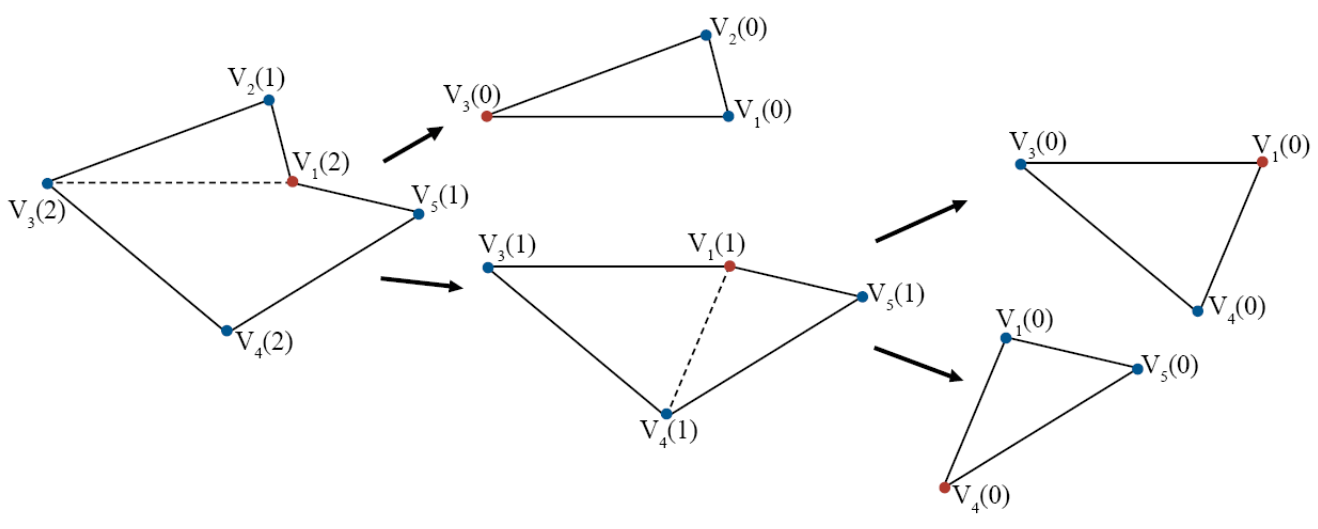
\includegraphics[width=1\textwidth]{bilder/sichtbarkeit_zerlegung.png}
    \caption[Triangulation mittels Sichtbarkeitsalgorithmus]{\centering Von links nach rechts die Schritte der Unterteilung eines Polygons in Unterpolygone bis zur Triangulierung mittels Sichtbarkeit der Eckpunkte (rot die First Heads)\cite{newAlg} }
\end{figure}
\pagebreak


\begin{table}[t]
    \begin{tabular}[h]{| c | c | c | c | c |}
    \hline
    \multicolumn{5}{|c|}{Eckenanzahl: 30 ~~~ $v_i = \left\{(x,y)| -50 < x < 50, -50 < y < 50\right\}$}\\ \hline
   Algorithmus & Polygon- & Durchschn.& Standartabw. & Durchschn. \\
   & fläche &  Dreiecksfläche & der Dreiecksfläche & min. Winkel \\ \hline
    Ear-Clipping & 4128,5px & 147,446px  & 163,63px  & 10,29° \\ \hline
    Sichtbarkeit & 4128,5px & 147,446px  & 148,91px & 15,04°\\ \hline
    \end{tabular}
    \caption[Vergleich \ac{eca} und Sichtbarkeitsalgorithmus bei rundem Polygon]{\centering Vergleich des \ac{eca} und des Sichtbarkeitsalgorithmus bei einem rundem Polygon mit 30 Ecken anhand der Standartabweichung der Dreiecksfläche in Pixeln (je kleiner desdo besser)
    und der durchschnittlichen minimalen Innenwinkelgröße in Grad (je größer desdo besser) \cite{newAlg}\linebreak\linebreak}
    \label{tab:tab2}
    
\end{table}

\begin{table}[t]
    \begin{tabular}[h]{| c | c | c | c | c |}
    \hline
    \multicolumn{5}{|c|}{Eckenanzahl: 30 ~~~ $v_i = \left\{(x,y)| -100 < x < 100, -30 < y < 30\right\}$}\\ \hline
   Algorithmus & Polygon- & Durchschn.& Standartabw. & Durchschn. \\
   & fläche &  Dreiecksfläche & der Dreiecksfläche & min. Winkel \\ \hline
    Ear-Clipping & 5066px & 180,93px & 185,50px & 9,23° \\ \hline
    Sichtbarkeit & 5066px & 180,93px & 146,03px & 16,45° \\ \hline
    \end{tabular}
    \caption[Vergleich \ac{eca} und Sichtbarkeitsalgorithmus bei länglichem Polygon]{\centering Vergleich des \ac{eca} und des Sichtbarkeitsalgorithmus bei einem länglichen Polygon mit 30 Ecken anhand der Standartabweichung der Dreiecksfläche in Pixeln (je kleiner desdo besser)
    und der durchschnittlichen minimalen Innenwinkelgröße in Grad (je größer desdo besser) \cite{newAlg}}
    \label{tab:tab3}
\end{table}
\break
\begin{flushleft}
    \vfill
\end{flushleft}



\section{Praktische Implementierung}

\subsection{Programmiersprache und Bibliotheken}
\subsubsection{Rust}
    Wie bereits im Abschnitt über verwandte Arbeiten angesprochen, sind wichtige Punkte bei der Implementierung von Algorithmen die 
    Geschwindigkeit und die Speichernutzung. Eine Programmiersprache, welche darauf ausgelegt ist in diesen Bereichen besonders effizient zu sein, 
    ist Rust. \cite{rust} Entworfen von Graydon Hoare, welcher seine Neuentwicklung im Juli 2010 das erste Mal  vorstellte, ist Rust eine sehr vielseitige Sprache.
    Mit dem Grundsatz einer open-source Multiparadigmen-Systemprogrammiersprache ist sie nicht nur für die breite Masse der Programmierer zugänglich, sondern auch 
    speziell für die Umsetzung von hardwarenaher Programmierung geeignet. Die Sprache setzt viele verschiedene Paradigmen der praktischen Programmierung um. So 
    unterstützt Rust sowohl funktionale als auch objektorientierte, sowie nebenläufige Programmierung. Auch ein hoher Abstraktionsgrad ist möglich. Vor allem aber 
    wurde beim Entwurf der Sprache darauf geachtet, dass die Kosten der Abstraktion zu Laufzeit so gering wie möglich sind. Man spricht von \emph{zero-cost-abstractions}, 
    welche beispielsweise auch bei der weitverbreiteten Programmiersprache \emph{C++} umgesetzt wurden. \cite{rust-wiki}
    Ein weiterer Vorteil von Rust ist, das die Sprache für \emph{cross-platform} Benutzung geeignet ist. Das bedeutet sie ist betriebssystemunabhängig. Das macht Rust zu einer 
    sehr einfach zugänglichen Sprache, da es nicht notwendig ist, ein UNIX-Basiertes- oder ein Windows-Betriebssystem zu besitzen oder gegebenenfalls ein Subsystem oder eine 
    Virtual Machine zu nutzen. All das würde zusätzlichen Aufwand bedeuten.
    Trotz allem sind natürlich, wie in keiner Programmiersprache, alle gewünschten Funktionen bereits implementiert. Bei Rust stellt das, durch den open-source Charakter,
    jedoch kein Problem dar. Die Community kann unter Nutzung des originalen Funktionsumfangs, der Standardbibliotheken, weitere neue Bibliotheken erstellen. 
    So ist beispielsweise die Bibliothek \emph{Iced} entstanden, welche für den Entwurf von \ac{gui}s gedacht ist. Im nächsten Kapitel ist darüber mehr zu lesen.
\subsubsection{Iced}
Wie bereits angedeutet, ist Iced eine Bibliothek für Rust, welche auf die Umsetzung von grafischen Nutzerinterfaces spezialisiert ist.
Der spanische Programmierer Héctor Ramón ließ sich bei Iced von der Sprache Elm inspirieren. Es ist zu erwähnen, dass sich Iced zum Zeitpunkt, da diese Arbeit verfasst wird, mit der Version 
0.4 noch im experimentellen Status befindet. Dennoch sind bereits die verschiedensten Funktionen nebst anschaulichen Beispielen für die Implementierung umgesetzt. Auch sind zwei verschiedene 
Renderer, also Software zum Darstellen von Grafiken auf dem Computerbildschirm, vorhanden. Namentlich \emph{iced-wgpu} und \emph{iced-glow}, unterstützt der erste der beiden die Verwendung von 
Vulkan \cite{vulkan}, Metal \cite{metal} und DirectX 12 \cite{dx12} und der zweite die Verwendung von OpenGL 2.1+ \cite{opgl} und OpenGL ES 2.0+ \cite{opgles}. \cite{iced}

\subsection{Entwurf des grafischen Nutzerinterfaces}
Eine Möglichkeit, um bereits in der Entwurfsphase auf Aspekte der Nutzerfreundlichkeit eingehen zu können, 
stellen Papierentwürfe dar. Dabei wird das \ac{gui}, statt aus digitalen Fenstern, aus einzelnen Blättern Papier gezeichnet und die Funktionen so simuliert. Dabei fallen negative Punkte wie zu tiefe oder breite 
Menüs auf und können direkt behoben werden, bevor sie schon im Code umgesetzt sind. Das vermeidet aufwendiges Umstrukturieren von hunderten Zeilen Code.

Bei dieser Arbeit gab es zwei konkurrierende Entwurfsideen, welche hier aus Gründen der Anschaulichkeit und Qualität nicht auf Papier dargestellt werden. Statt dessen werden digitale Skizzen verwendet, bei denen eventuelles Auffalten des Papiers
durch Pfeile und Beschriftung gekennzeichnet werden. 
Die Ideen unterscheiden sich vor allem durch das erste Menü, welches einmal die Optionen für die Triangulation inkludiert - im Folgenden als \emph{Menü Entwurf - Optionen inkludiert} und einmal ein Entwurf, bei dem 
die Optionen auf einem extra Menü nach Eingabe des Polygons aufgeführt werden. Dieser zweite Entwurf soll als \emph{Menü Entwurf - Optionen nachfolgend} bezeichnet werden.
Klar war jedoch von Beginn an, wie die Algorithmusiteration aussehen soll. Sie wird im Abschnitt \emph{Iteration Entwurf} dargestellt.
Zuletzt soll das Resultat des Algorithmus gezeigt werden. Auch hierfür gab es zwei unterschiedliche Konzepte. Einmal sollten zwei Anzeigen umgesetzt werden, zum einen das Ergebnis des gewählten Algorithmus und zum anderen das 
Ergebnis aus einer \ac{dt}, welche als optimales Ergebnis gilt und einen guten Qualitätsvergleich ermöglicht. Dieser Entwurf wird als \emph{Resultat Entwurf - Vergleichsfenster} bezeichnet.
Der andere Entwurf wird aufgrund der hier nur textlich dargestellten Metadaten als \emph{Resultat Entwurf - Metadaten} bezeichnet.


\subsubsection{Menü Entwurf - Optionen nachfolgend}
\raggedbottom
Dieser Entwurf sollte das Zeichen des Polygons in den Vordergrund stellen. Damit der Nutzer nicht von allen Optionen erschlagen wird, sondern diese nach und nach abarbeitet, wurden die Einstellungen in ein zweites Fenster 
ausgelagert. \pagebreak

\begin{figure}[t]
    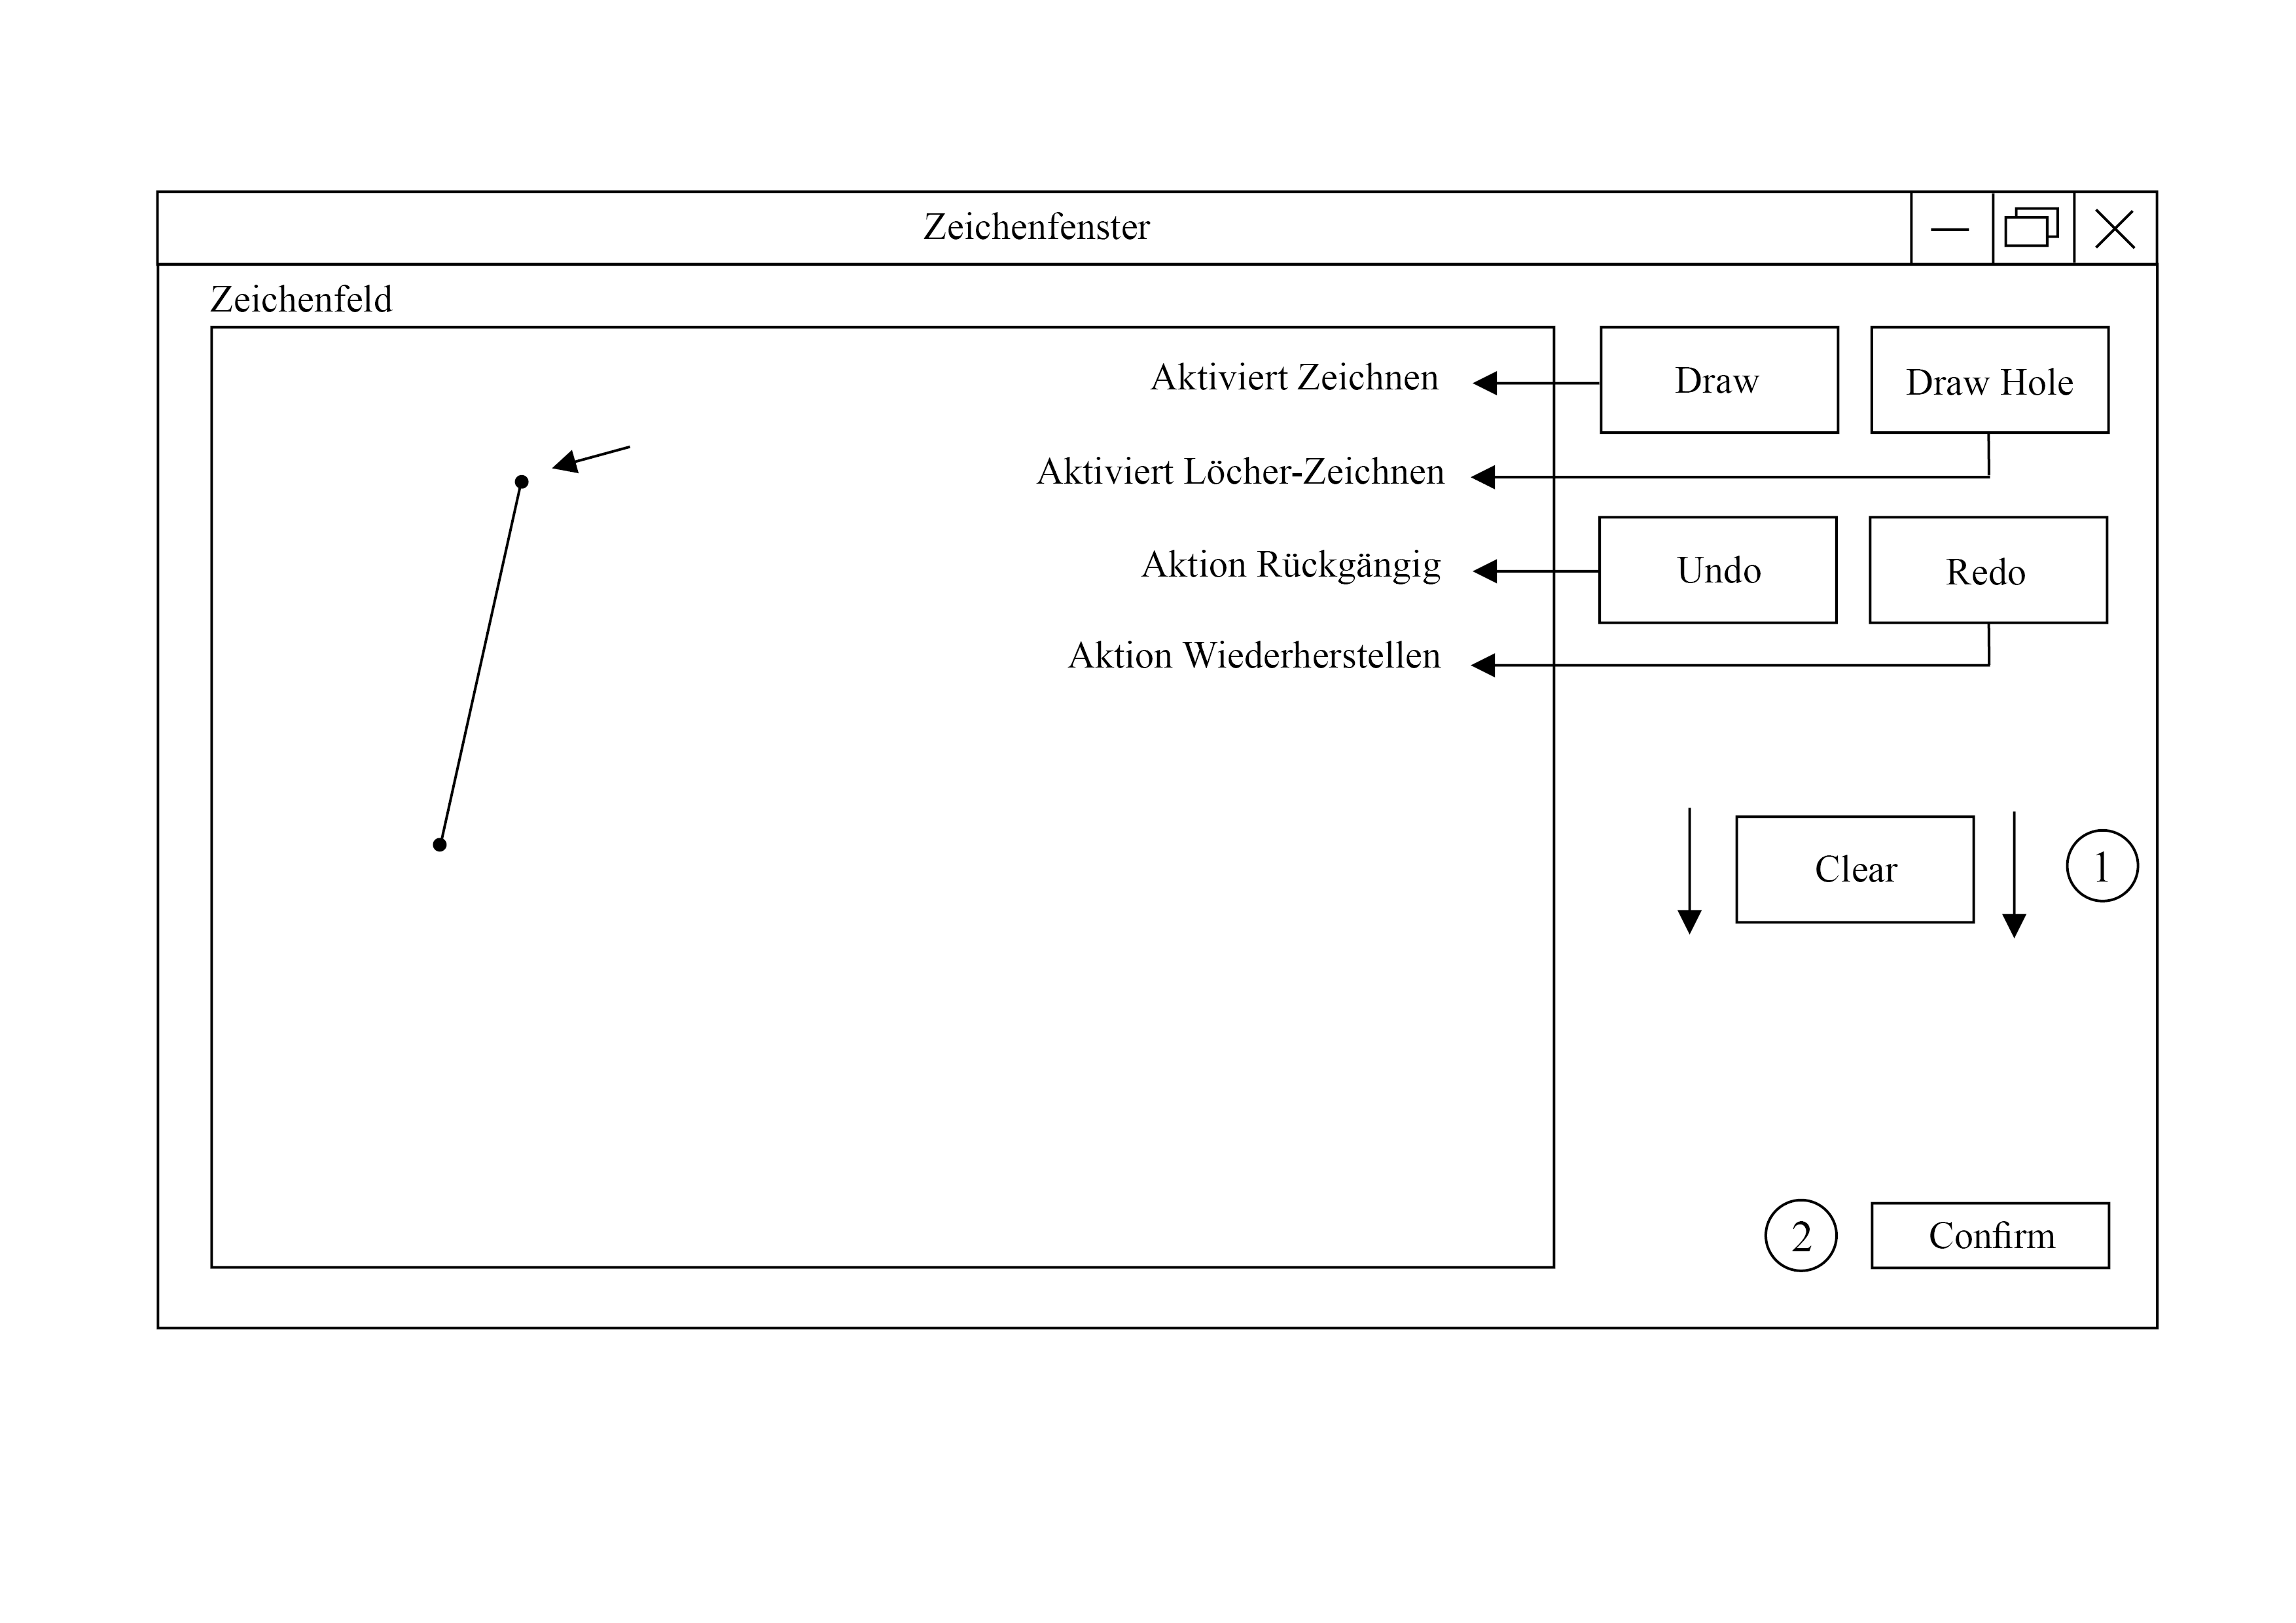
\includegraphics[width=0.9\textwidth]{bilder/menu_ohne_optionen.png}
    \caption[Entwurf des Menüs mit nachfolgenden Optionen]{Entwurf des Menüs mit nachfolgenden Optionen. links: Zeichenfeld für Eingabe des Polygons, rechts: Buttons mit Einfluss auf das Zeichenfenster. (1) öffnet Diaglogfenster (siehe Abbildung \ref{fig:cleardia})
    (2) Bestätigung des Polygons und Übergang in das Optionsfenster (siehe Abbildung \ref{fig:options})}
    \label{fig:menu_ohne_optionenen}
\end{figure}

Dieses erscheint nach Eingabe und Bestätigng des Poylgons durch Drücken auf den \emph{Confirm-Button}.(siehe Abbildung \ref{fig:options}) Dieser Fensterwechselt wurde mit der Nummer (2) gekennzeichnet. Die Buttons, welche sich alle in einer Box an der rechten Seite des Zeichenfeldes befinden, haben alle eine Funktion,
\begin{wrapfigure}{h}{0.6\textwidth}
    \centering
    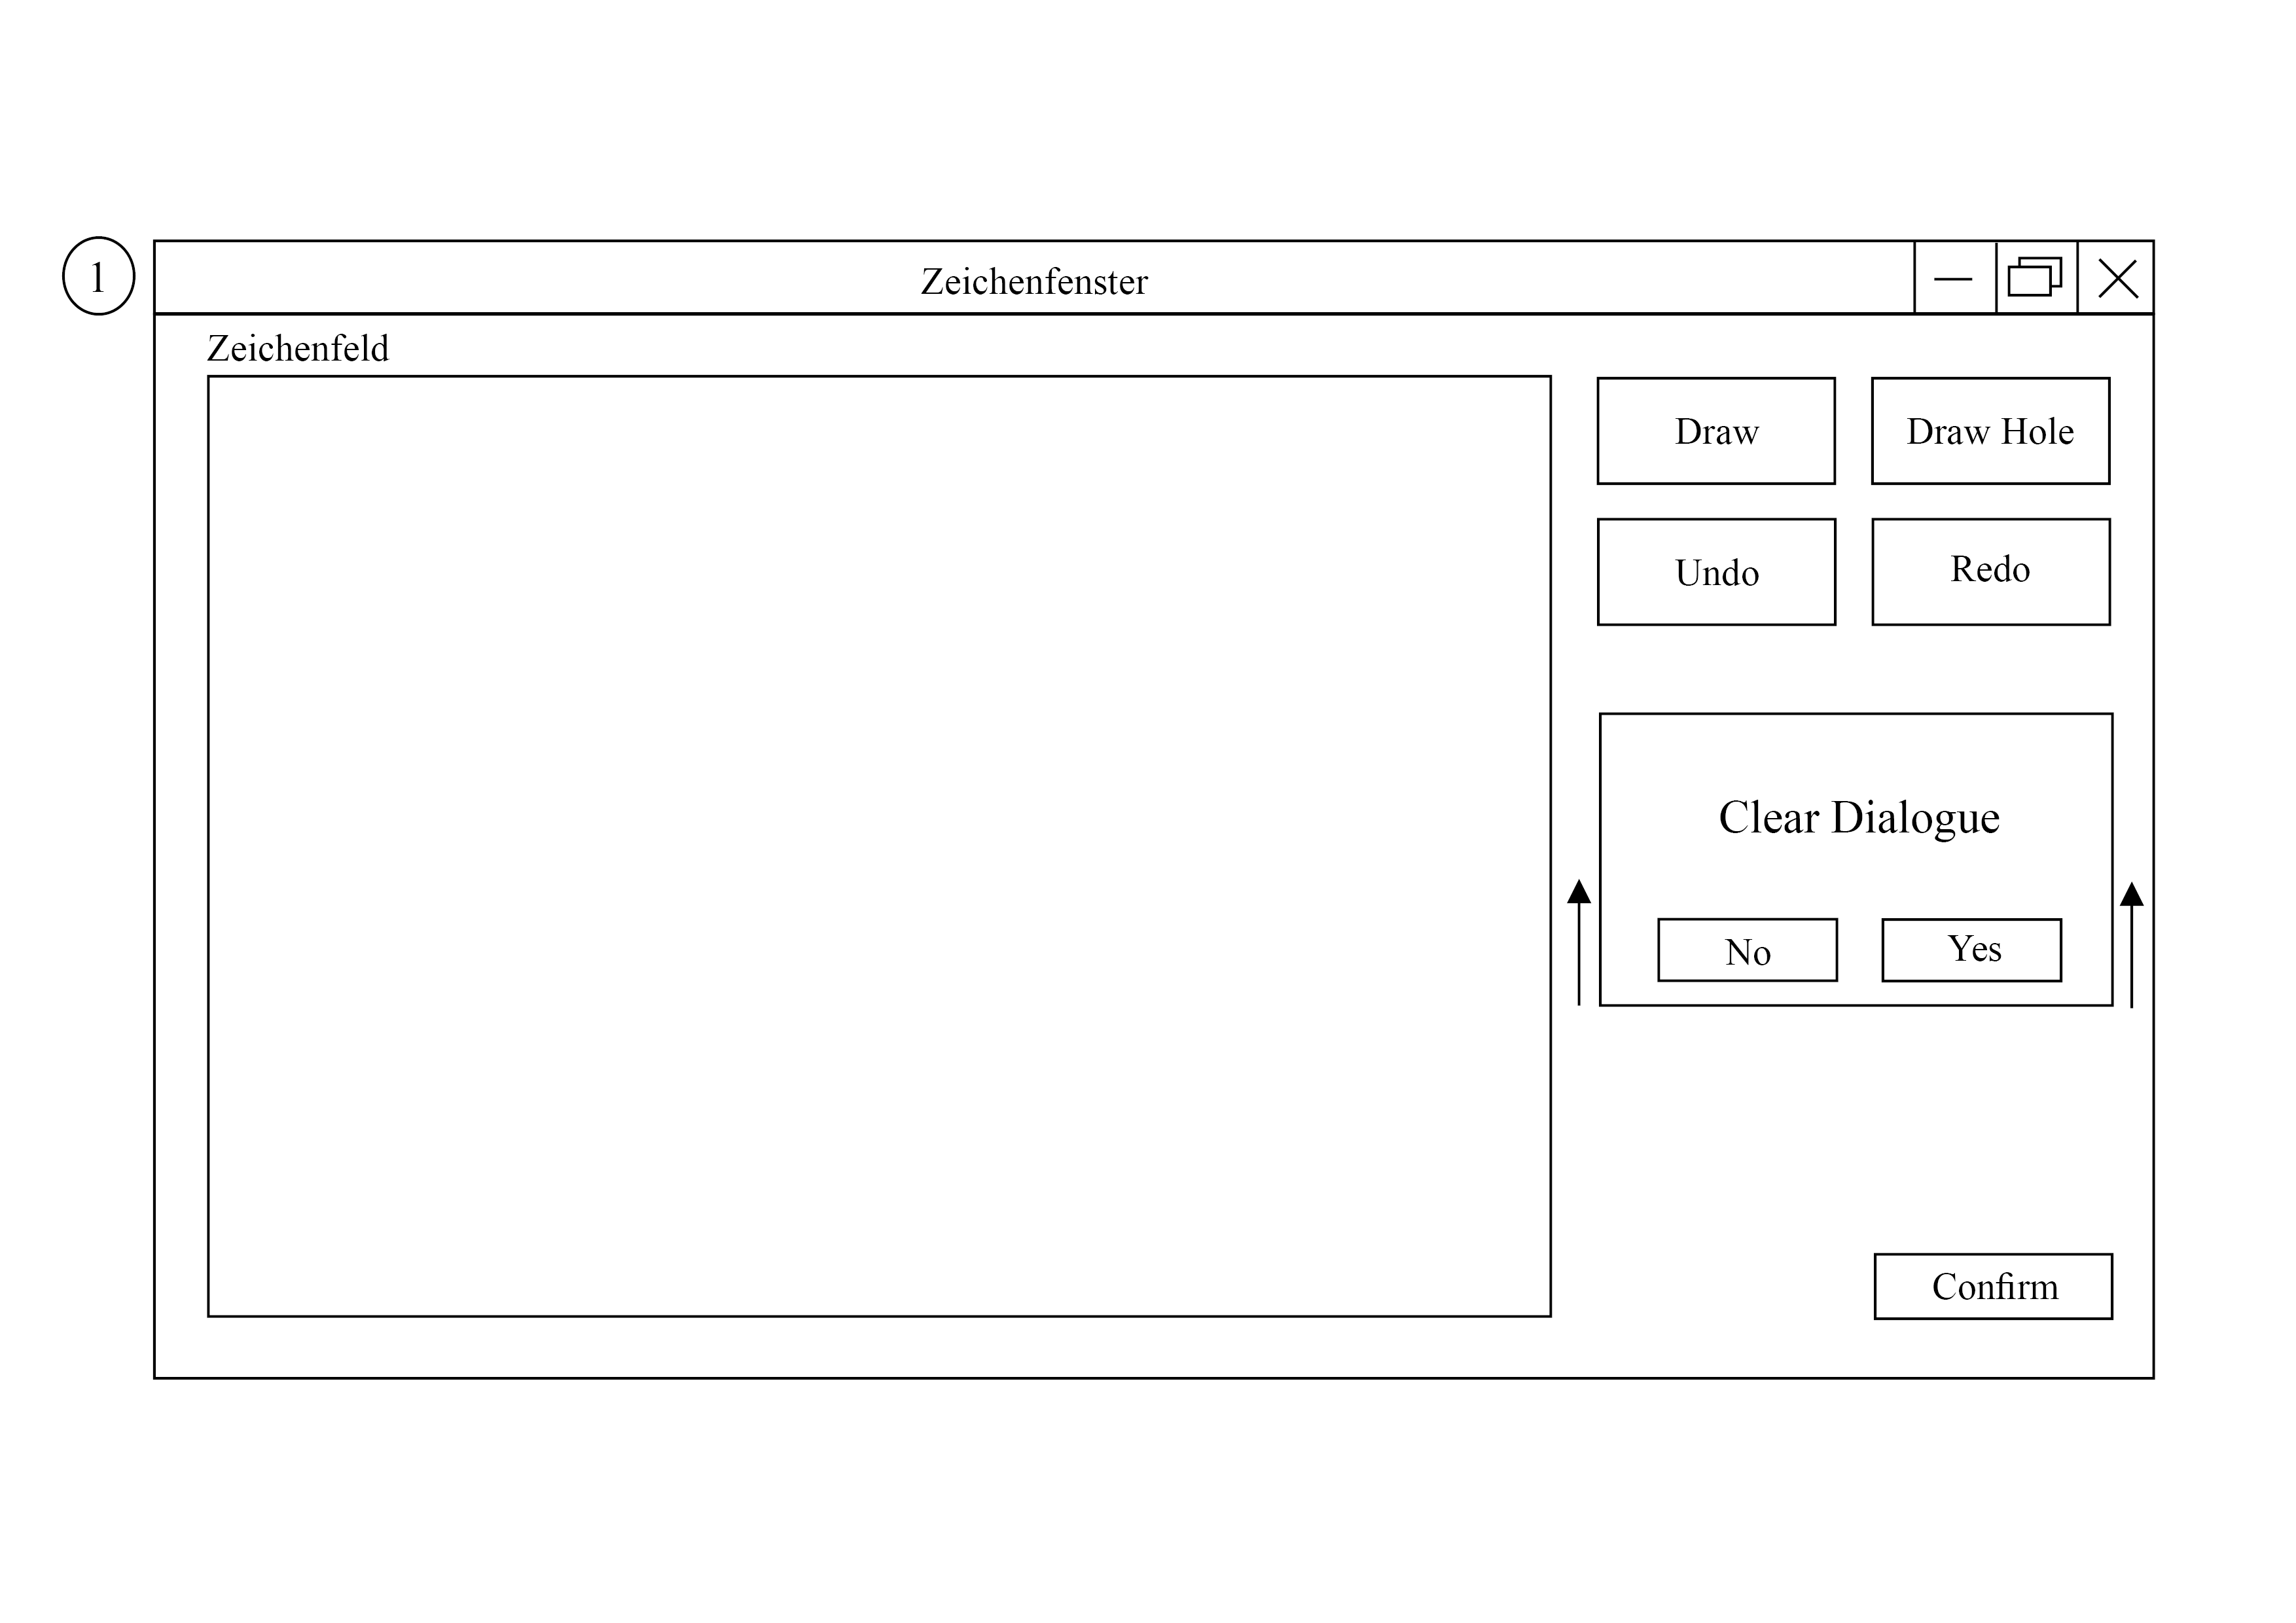
\includegraphics[width=0.6\textwidth]{bilder/cleardialogue.png}
    \caption[Öffnung des Dialogfensters]{Dialogfenster wurde durch bedienen des \emph{Clear-Buttons} aufgeklappt. Bestätigung oder Ablehnung durch den Nutzerw wird erwartet.}
    \label{fig:cleardia}
\end{wrapfigure}
welche das Zeichenfeld beeinflusst. 
Die Ausnahme ist hierbei der bereits angesprochene \emph{Confirm-Button}, welcher das eingegebene Polygon bestätigt und dann das Fenster mit den Optionen aufruft.
Der Einfluss der Buttons auf das Zeichenfenster ist mittels Pfeilen dargestellt, da sich augenscheinlich nichts am Aussehen des Fensters ändert.
Der \emph{Clear-Button} besitzt Pfeile nach unten. Dies soll den Übergang (1) andeuten. Dabei klappt ein Diaglogfenster an der Stelle dieses Buttons auf. Es ist dazu gedacht, um eine versehentliche Löschung aller Eingaben auf dem Zeichenfeld zu vermeiden.
Der Nutzer muss die Löschen-Aktion hier nocheinmal bewusst bestätigen. Wurde dieser Dialog beendet, dann klappt das Dialogfenster wieder zu und der  \emph{Confirm-Button} wird wieder sichtbar. Nachfolgend ist der Entwurf in digitaler Form zu sehen.    
    \begin{figure}[h]
        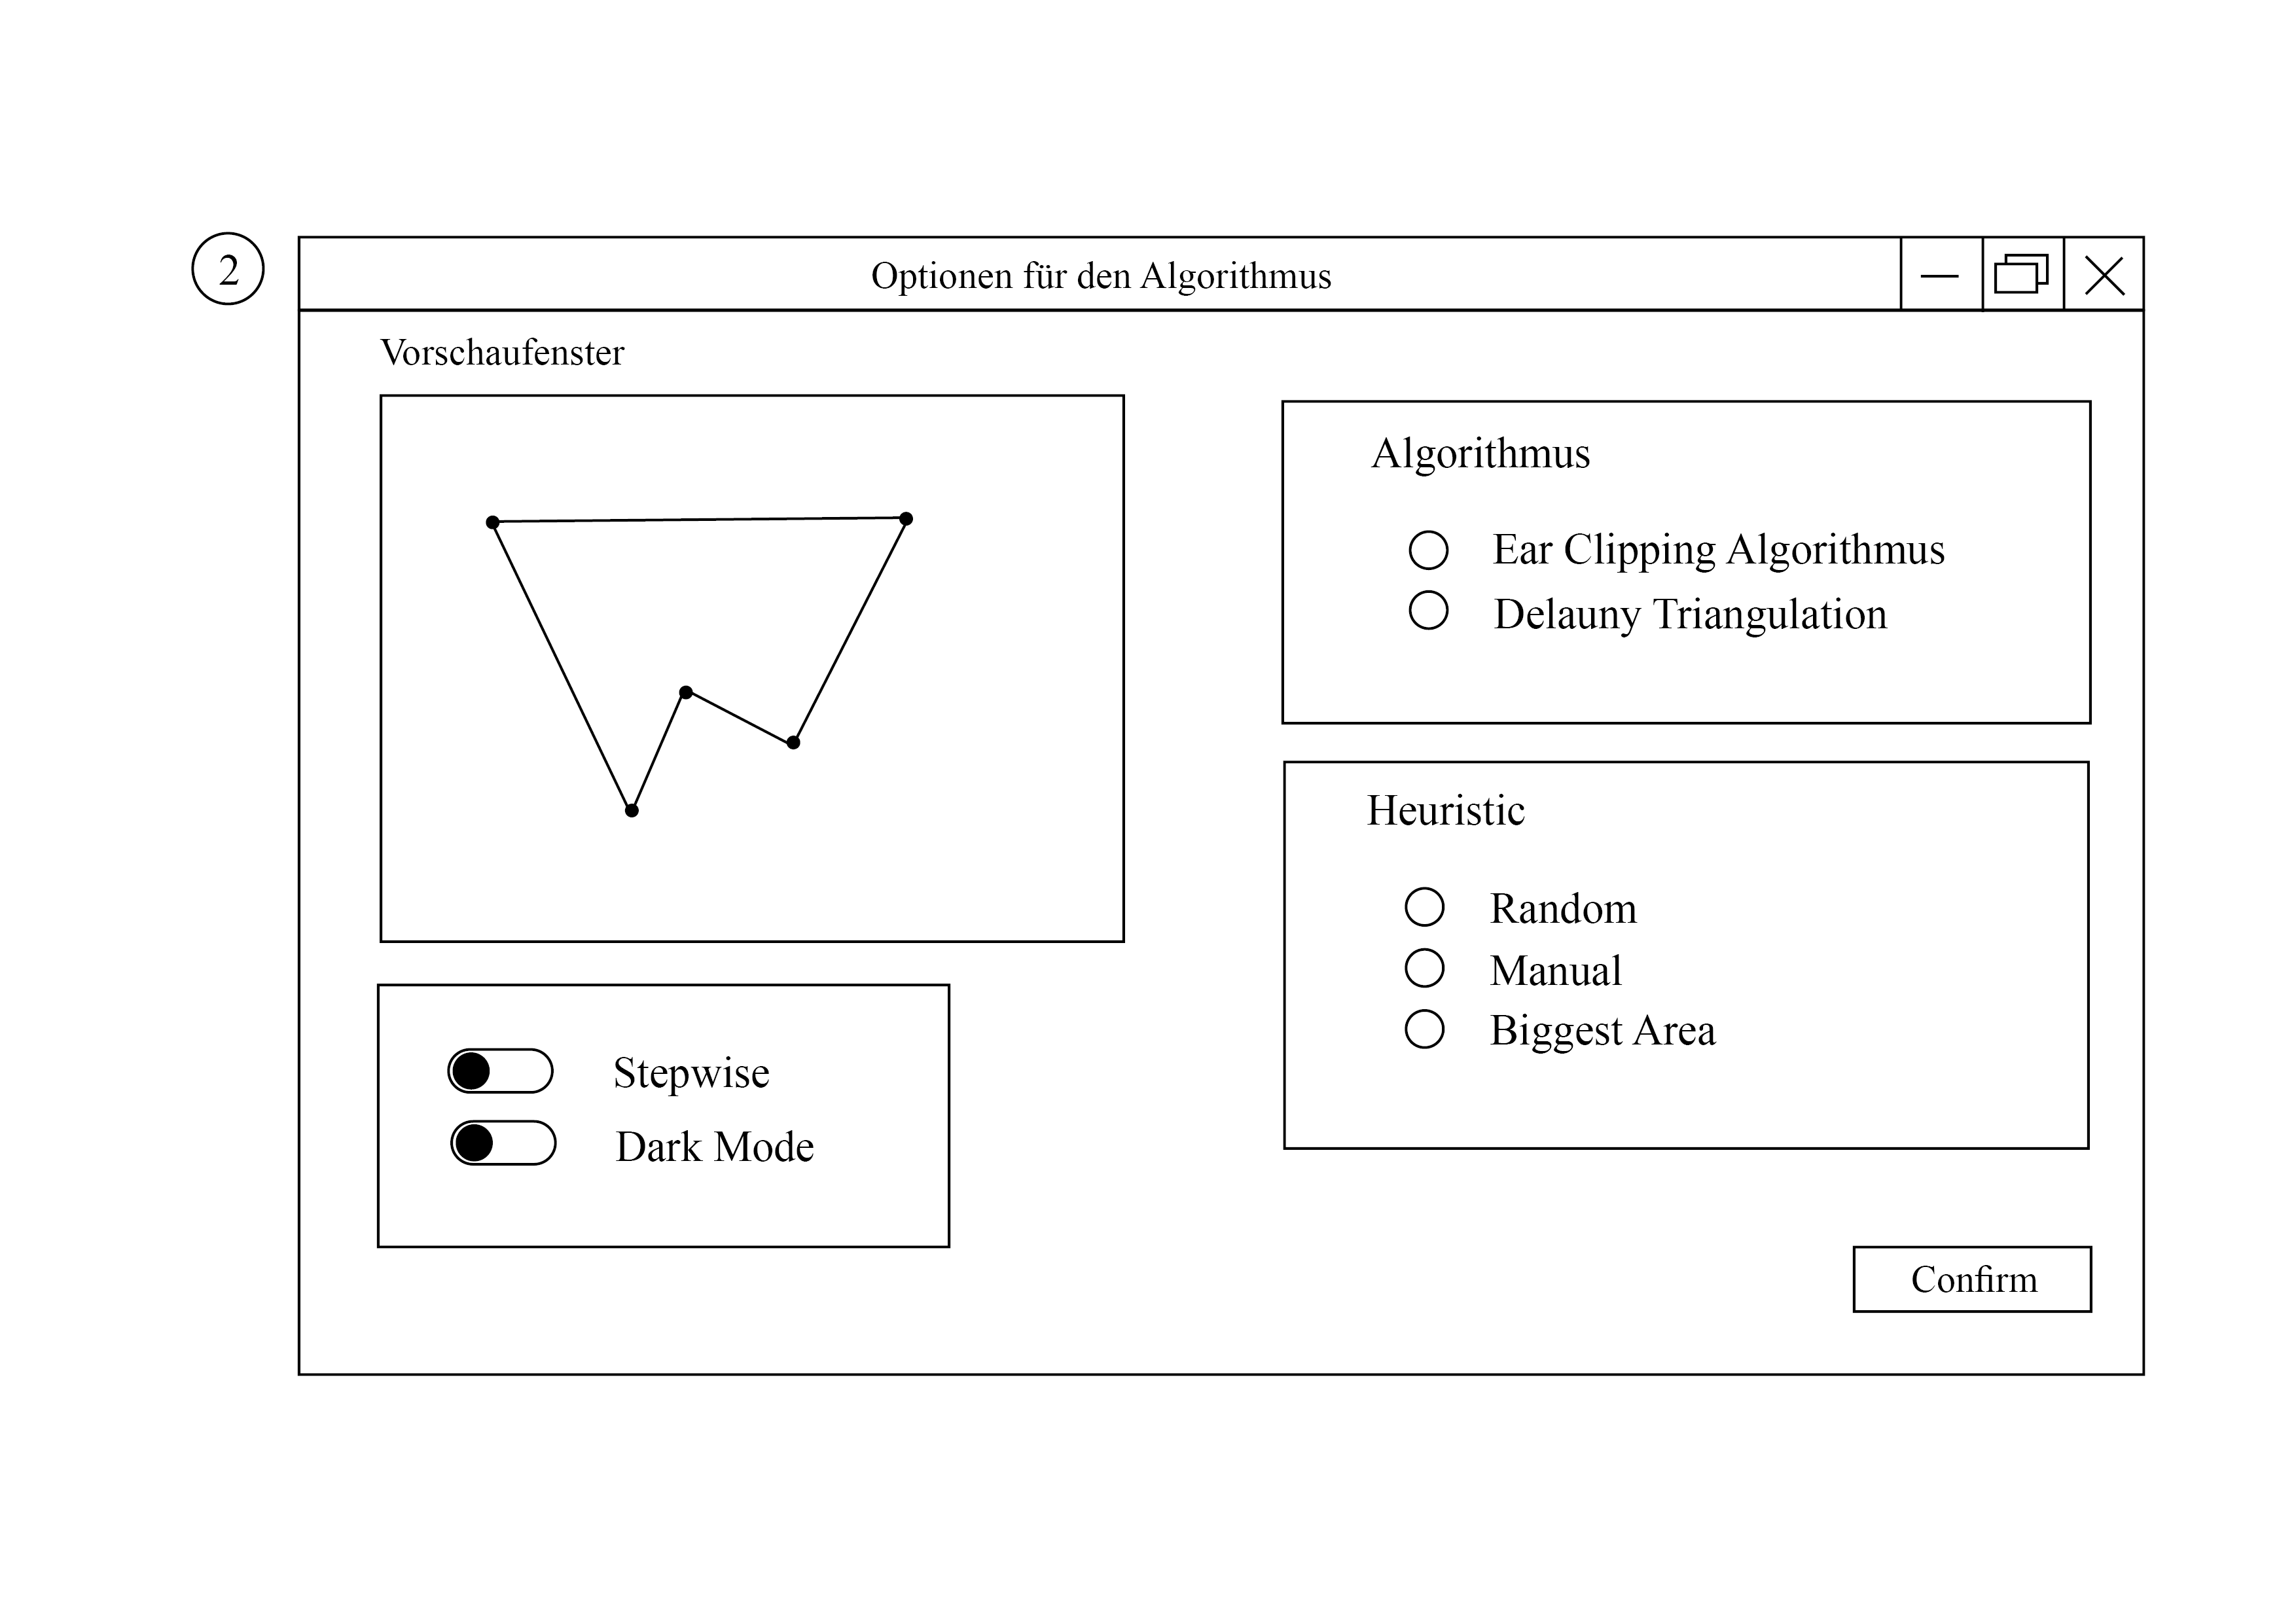
\includegraphics[width=1\textwidth]{bilder/optionsfenster.png}
        \caption[Ausgelagertes Optionsfenster]{Fenster, welches alle Optionen für den Algorithmus und die Software enthält. links: Vorschaufenster, darunter allgemeine Optionen. rechts: Algorithmus
        Auswahl und Auswahlt der Heuristik}
        \label{fig:options}
    \end{figure}

Wie in Abbildung \ref{fig:options} zu sehen ist, besteht das Optionsfentser aus vier Teilen. Oben links befindet sich das Vorschaufenster, welches das zuvor eingegebene Polygon zeigt. Es soll die gedankliche Verknüftung der Eingabe zu den Optionen herstellen.
Darunter befindet sich eine Gruppe von Togglern, welche die allgemeinen Optionen für die Ausführung des Algorithmus und das Aussehen der Anwendung beeinhalten.
Auf der rechten Seite befinden sich zwei Boxen, welche je eine Gruppierung von Radio Buttons umfassen. Die obere beinhaltet die Auswahl des Algorithmus. Die untere stellt die Auswahl der anzuwendenden Heuristik dar.
Durch einen weiteren \emph{Confirm-Button} wird der Übergang zur Iterationsseite geregelt.

Ein starker Nachteil dieses Entwurfs ist, dass alle Optionen, auch die allgemeinen, erst nach der ersten Eingabe zugänglich sind. Für das An- und Ausschalten des 
Dark Modes ist das unvorteilhaft. Auch sind nicht so viele Optionen vorhanden, dass der Nutzer überfordert werden könnte. 

Als vorteilhaft hingegen hat sich die Gruppierung der Buttons sowie der Radio Buttons erwiesen. Diese Unterstützung für den Nutzer, welche Bedienelemente zur selben Klasse gehören, stellte sich als positiv heraus.
Auch der Dialog zur Bestätigung des Löschens vermeidet eine Fehlbedienung und ist damit positiv zu bewerten.

\subsubsection{Menü Entwurf - Optionen inkludiert}
Der zweite Entwurf für das Menü beinhaltet auch die Optionen. Dies soll dem Nutzer alle Möglichkeiten auf einen Blick darbieten. Da es nicht sehr viele Auswahlmöglichkeiten gibt, sollte dieser Entwurf nicht zu Überforderung
des Benutzers führen. Im vorangegangenen Kapitell wurden einige Entwurfsstechniken angewendet, welche sich als vorteilhaft erwiesen. Hier sind zum Beispiel der Bestätigungsdialog und die Gruppierung ähnlicher Elemente zu nennen.
Diese wurden in diesen zweiten Entwurf übernommen. Auch bleibt das Zeichenfeld der größte Bereich des Menüs, um dieses in den Mittelpunkt der Anwendung zu stellen.

\begin{figure}[h]
    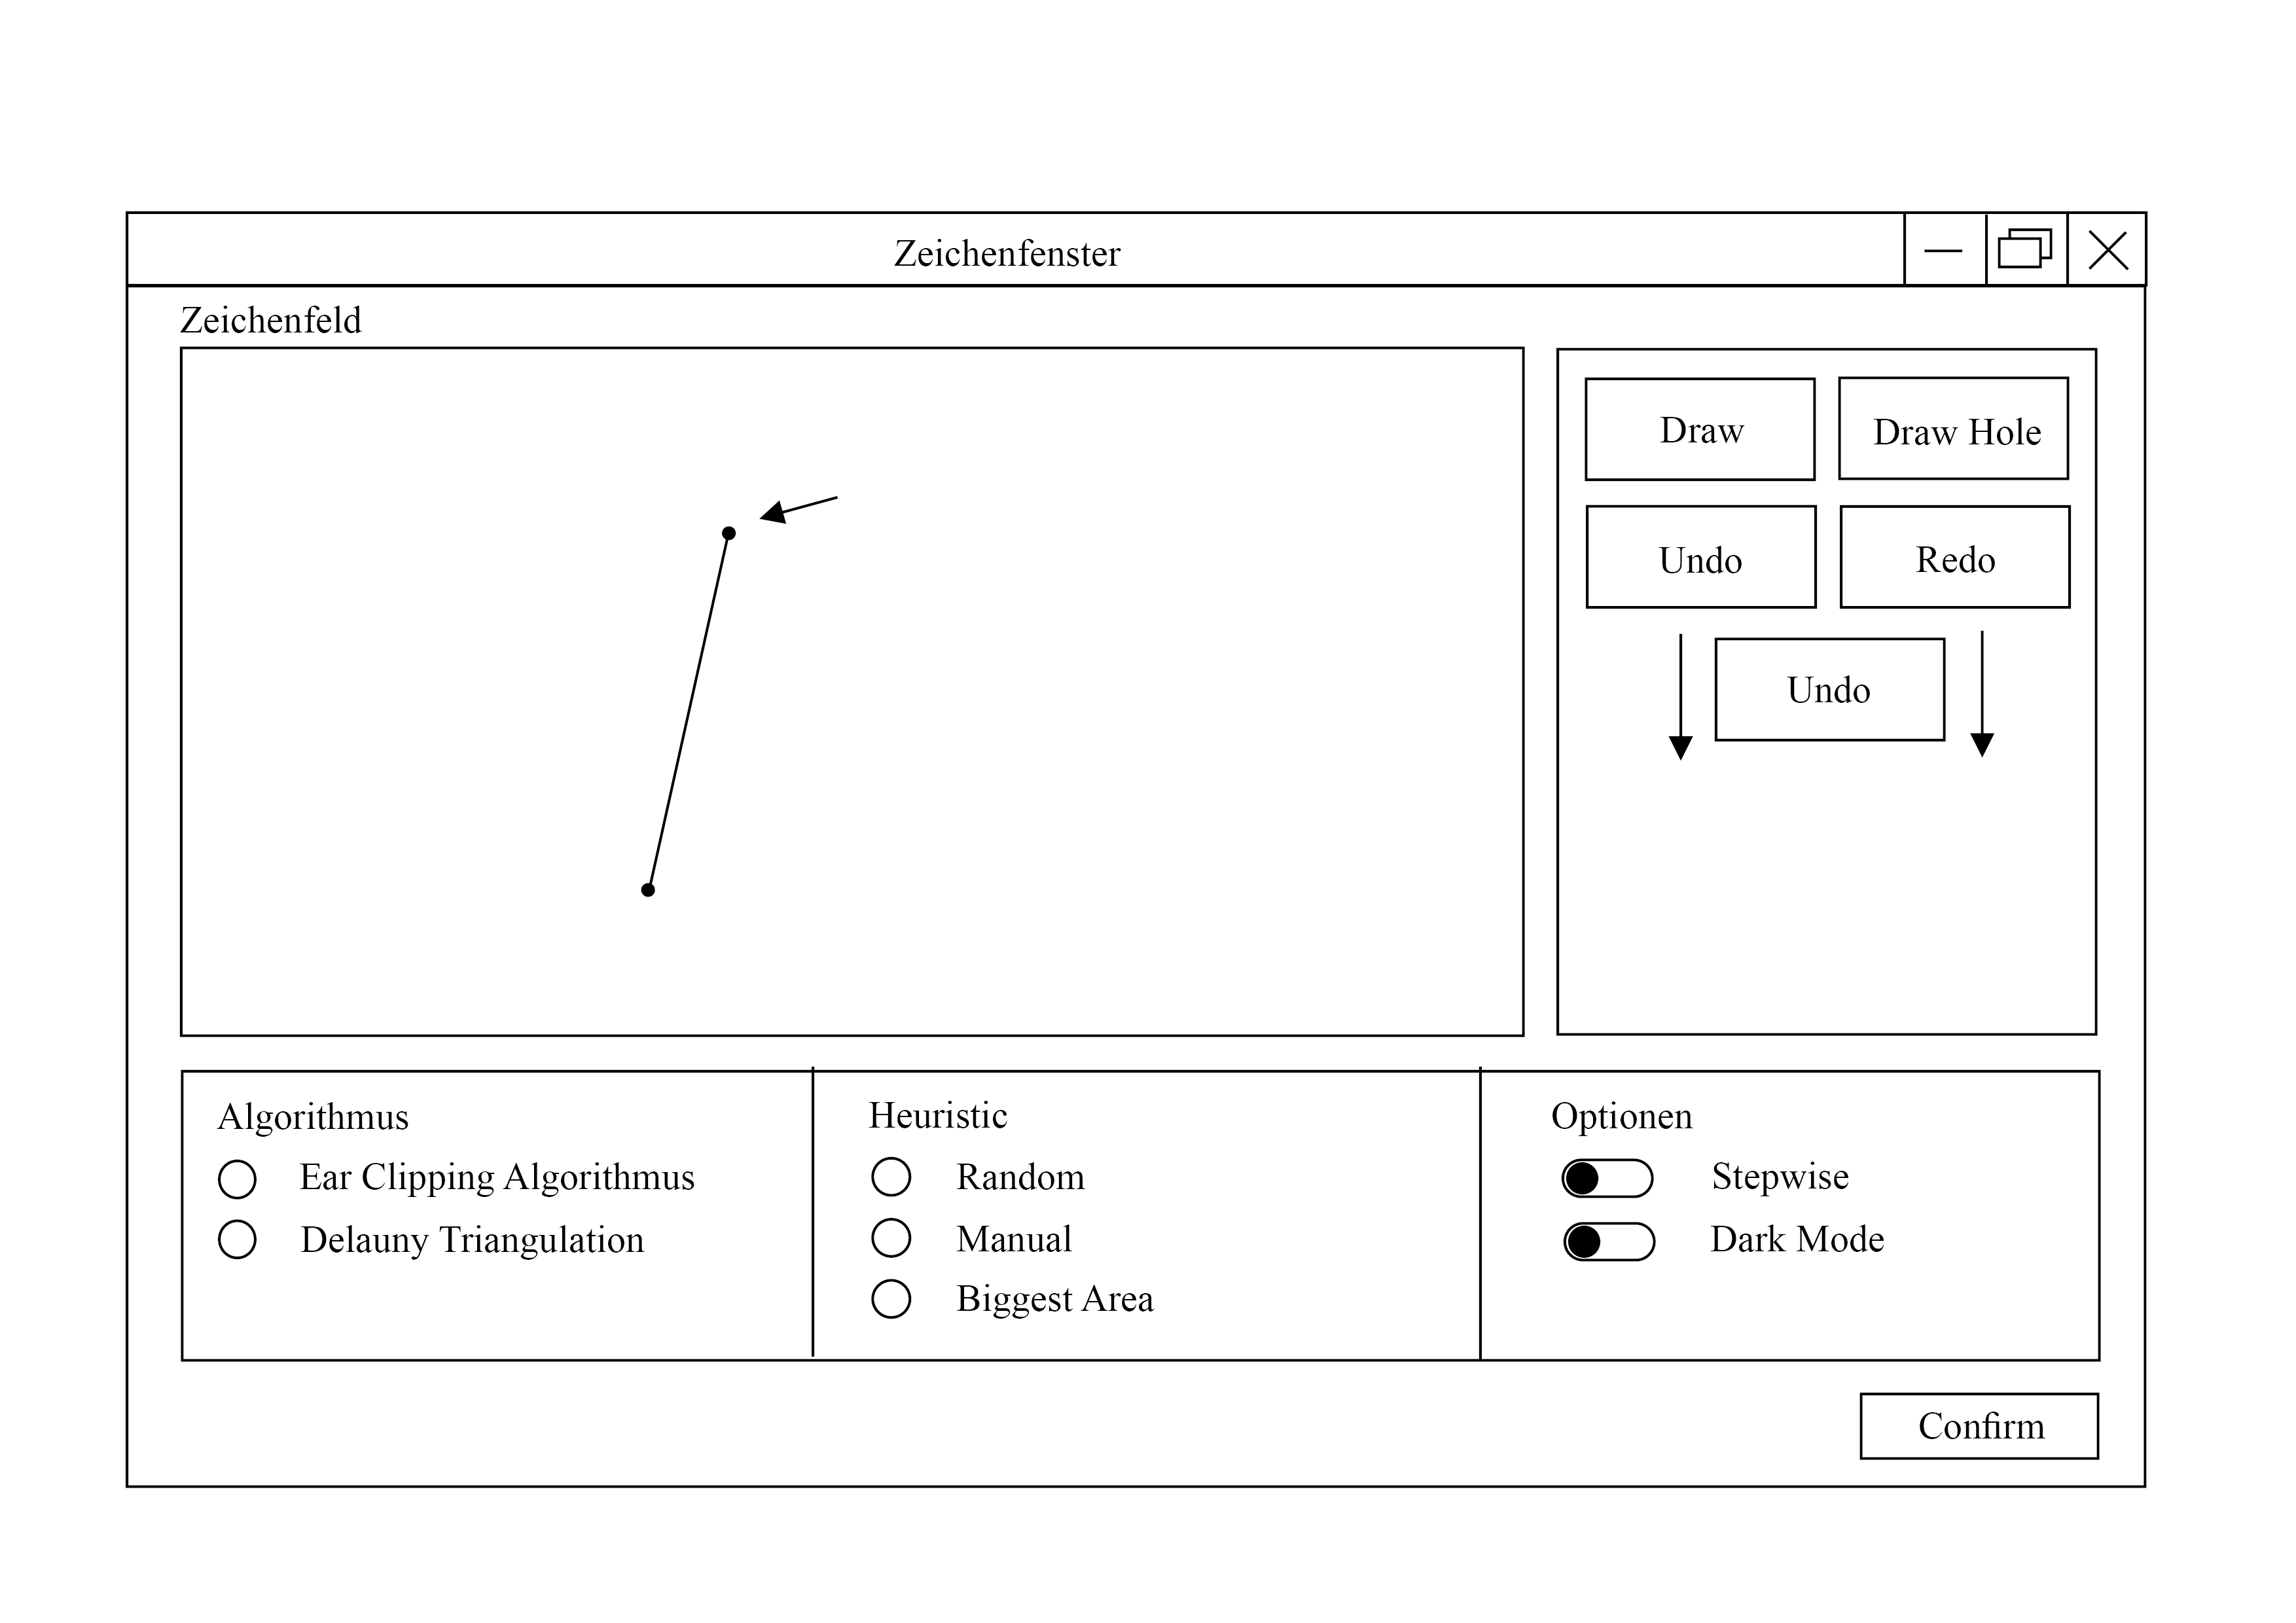
\includegraphics[width=1\textwidth]{bilder/menu_mit_optionen.png}
    \caption[Entwurf für das Menü mit Optionen]{Menü ähnlich dem Entwurf mit ausgelagerten Optionen. Hier im unteren Bereich drei Sektionen für die Einstellungsmöglichkeiten.}
    \label{fig:menu_mit_optionen}
\end{figure}

Wie in der Abbildung \ref{fig:menu_mit_optionen} zu sehen ist, wurde der \emph{Confirm-Button} aus der Gruppe der Zeichenwerkzeuge ausgelagert. Das hat den Grund, dass er nicht nur die Zeichnung sondern auch alle gewählten Optionen bestätigt.
Daher befindet er sich ganz unten rechts. Auch in den folgenden Entwürfen wird der Button für den Übergang zur nächsten Seite an dieser Stelle sein. Somit ist einen gewisse Einheitlichkeit gewährleistet.
Die nächste Seite, welche durch den \emph{Confirm-Button} aufgerufen wird, ist, anders als im vorangegangenen Entwurf, sofort die Iterationsseite, nicht eine weitere Seite mit Optionen.
Die anderen Funktionen der Buttons und Optionen wurden bereits in Kapitel 4.2.1 beschrieben und sollen daher nicht an dieser Stelle erneut thematisiert werden.

\subsubsection{Iteration Entwurf}
Die Iterationsseite bestitzt eine klar definierte Funktion. Sie soll den Algorithmus schrittweise darstellen. Dafür bedarf es lediglich weniger Interaktionselemente. 
Zu allererst wird ein Vorschaufenster benötigt. Dieses steht im Mittelpunkt und ist daher besonders groß. Darunter befindet sich links ein Button, welcher es ermöglicht, die Schritte rückwärts darzustellen. Das funktioniert allerdings nur,
solange mehr als ein Schritt druchlaufen wurde. In der Mitte des unteren Randes befindet sich eine Fortschrittsanzeige, welche die Rückkopplung zum Nutzer darstellt. Hier wird der aktuelle Schritt in Relation zur gesamten Schrittanzahl gezeigt.
Rechts davon befindet sich der \emph{Next-Button}. Wird dieser gedrückt, dann wird auf dem Vorschaufenster der nächste Iterationsschritt angezeigt und die Fortschrittsanzeige einen Zähler nach oben gestellt.
Sind alle Schritte abgearbeitet, dann wird über den \emph{Next-Button} die nächste Seite, die Ergebnisseite, aufgerufen.

\begin{figure}[h]
    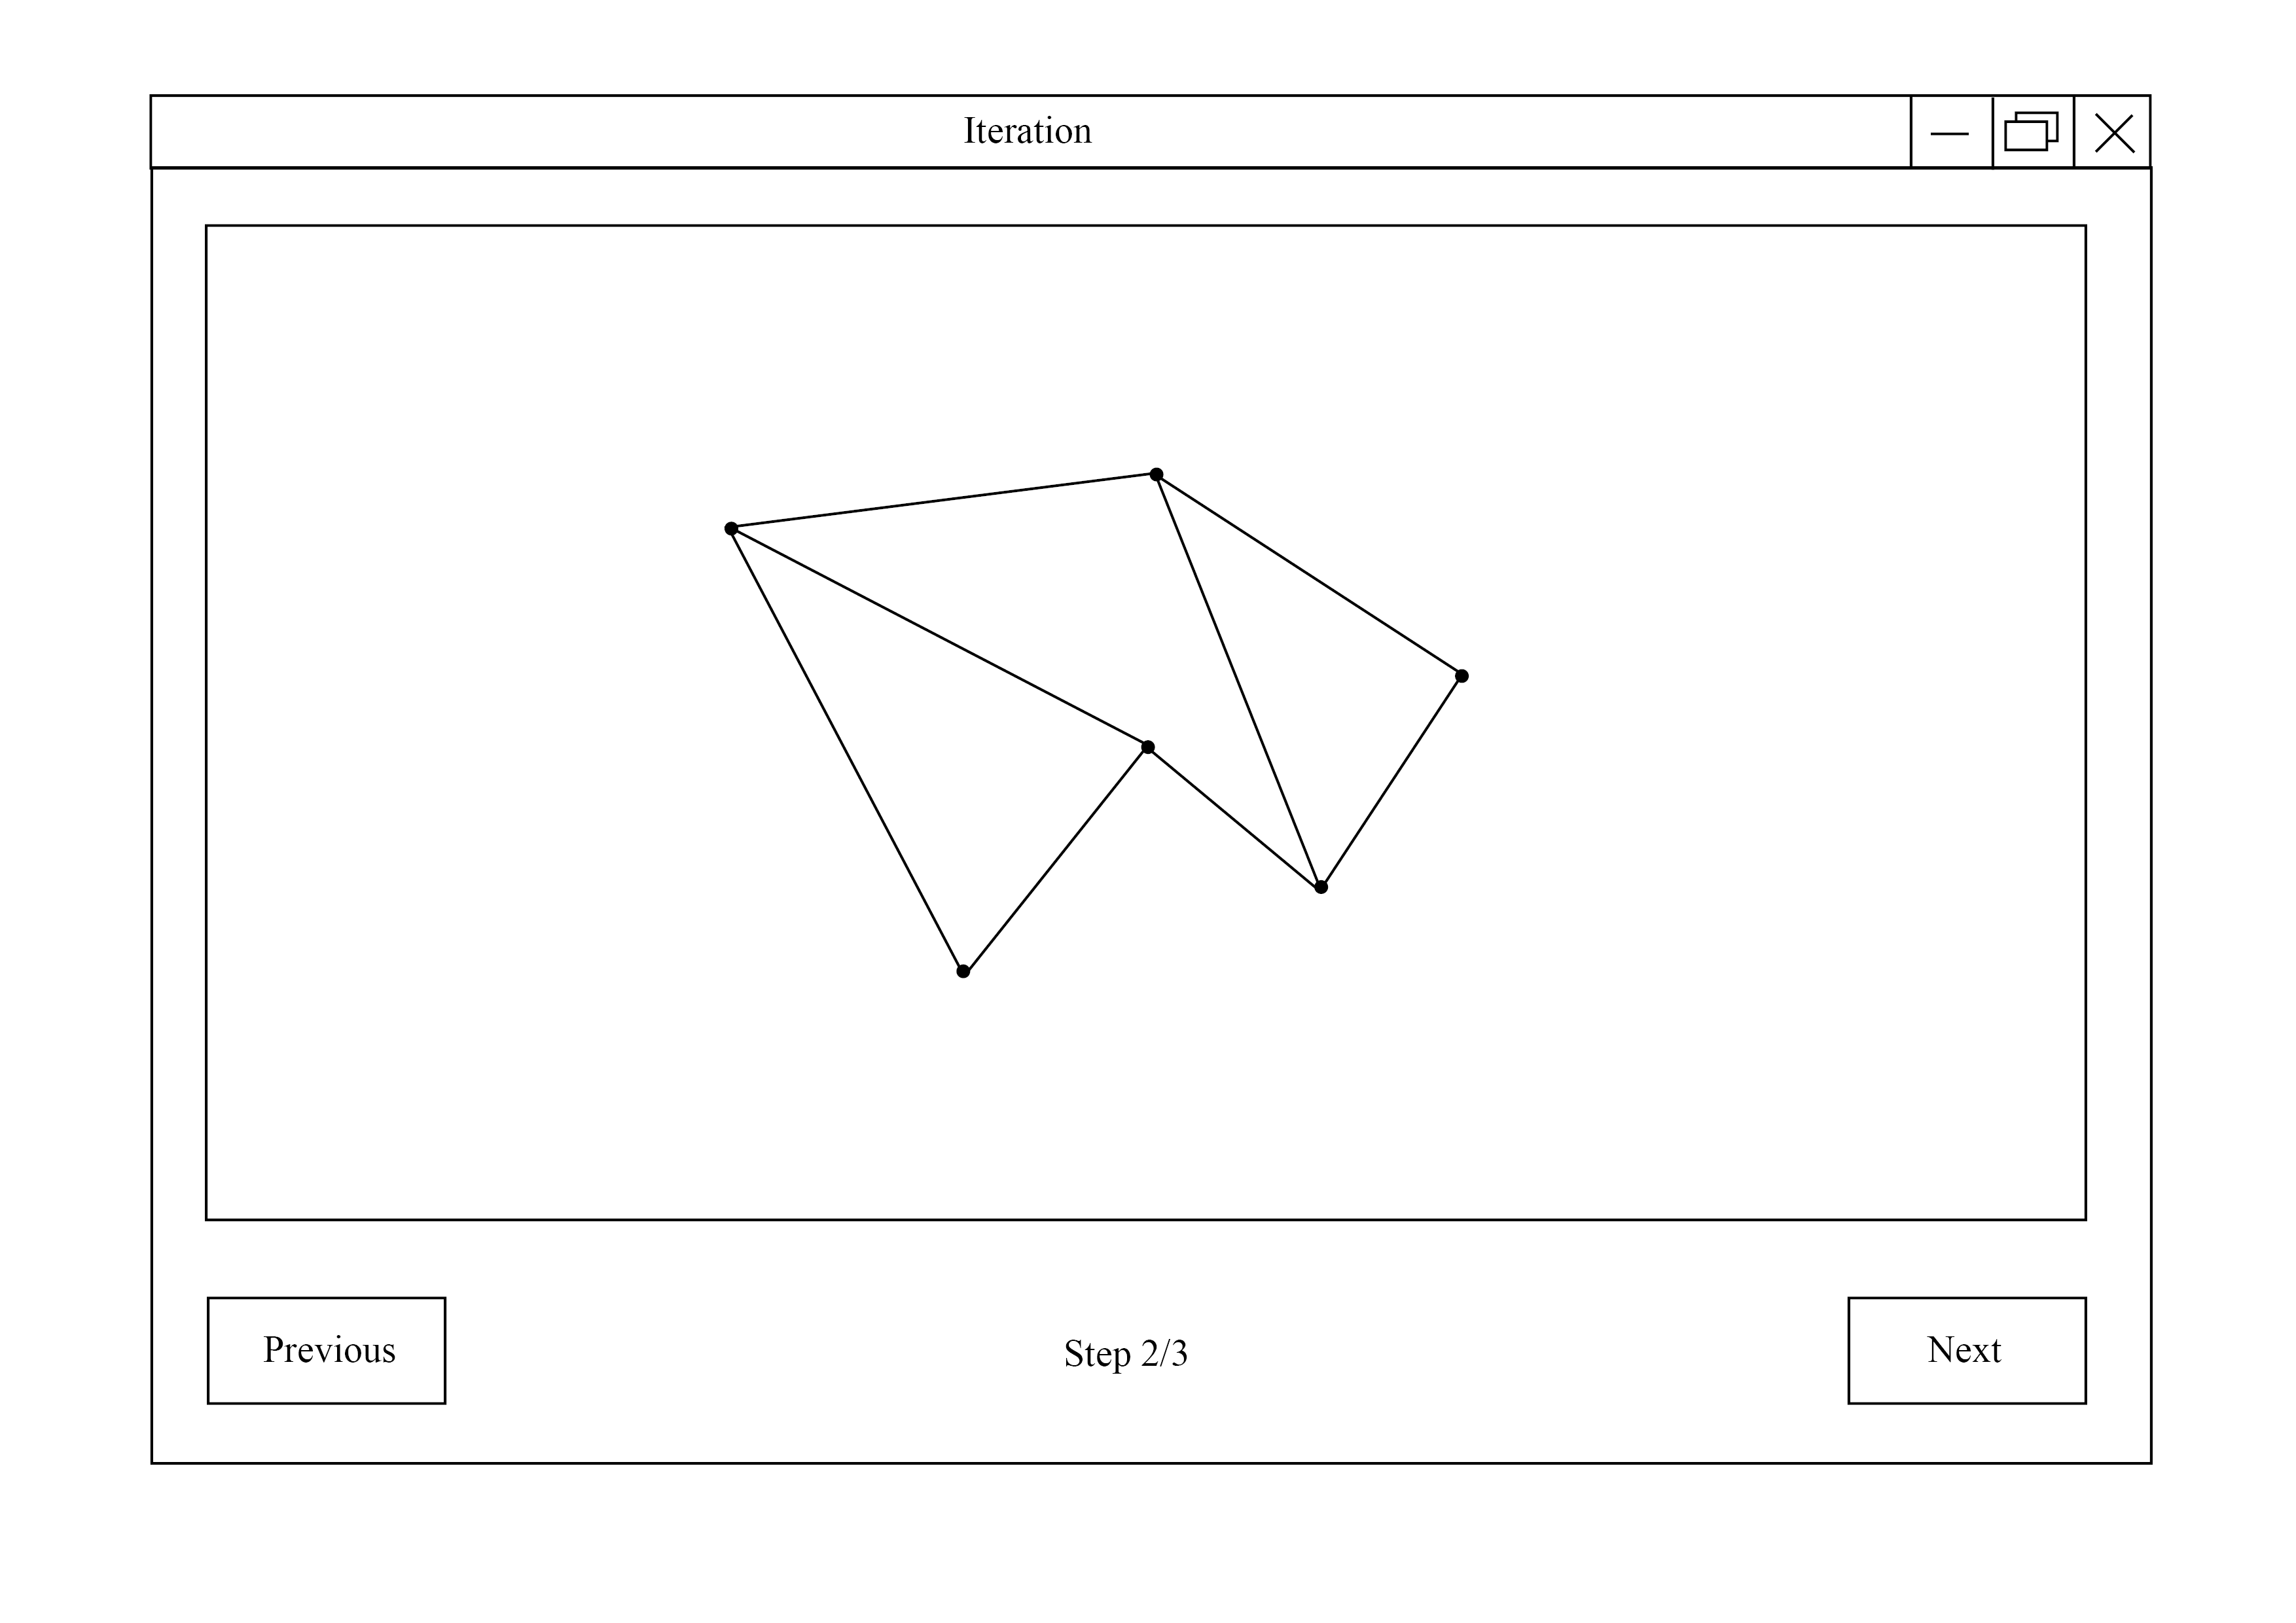
\includegraphics[width=1\textwidth]{bilder/iteration.png}
    \caption[Entwurf Iterationsseite]{Iterationsseite aus Vorschaufenster und Navigationsleiste mit Fortschrittsanzeige}
    \label{fig:iteration}
\end{figure}

Eine Entwurfsverbesserung, welche zu einem späteren Zeitpunkt aufkam, war, dass der \emph{Next-Button} nachdem der letzte Iterationsschritt durchgeführt wurde, seine Beschriftung auf \emph{End} wechselt.
Das soll beim Nutzer die Assoziation wecken, dass der Iterationsprozess abgeschlossen ist. Der Übergang auf die Ergebnisseite wird damit besser an den Anwender vermittelt.

\subsubsection{Resultat Entwurf - Metadaten}
Der erste Entwurf für die Ergebnisseite, auf welcher das Resultat der Algorithmusiteration zu sehen sein soll, umfasst wie die Iterationsseite nur drei Elemente.
Das Ergebnisfenster, welches das zerlegte Polygon zeigt, ist dabei fast seitenfüllend und damit das Zentrum der Betrachtung.
Darunter ist auf der linken Seite der \emph{Exit-Button}. Dieser beendet das Programm. Sein Gegenstück befindet sich auf der rechten Seite. Der \emph{Return-to-Menu-Button} (im Folgenden \emph{Return-Button})  
lässt den Nutzer, wie die Aufschrift bereits andeutet, auf die Menüseite zurückkehren. Dort wird das zuvor eingegebene Polygon im Zeichenfeld angezeigt. Es kann jetzt verändert werden. Auch können andere Einstellungen getroffen werden 
und der Algorithmus dann erneut durchgeführt werden.

Da allerings eine reine Anzeige des zerlegten Polygons wenig über seine Qualität aussagt, wurde dieser Entwurf noch angepasst. Unter dem Ergebnisfenster werden noch einige Daten über das Polygon und die Dreiecke dargestellt, welche die Zerlegung bilden.
Das sieht dann wie folgt aus:

\begin{figure}[h]
    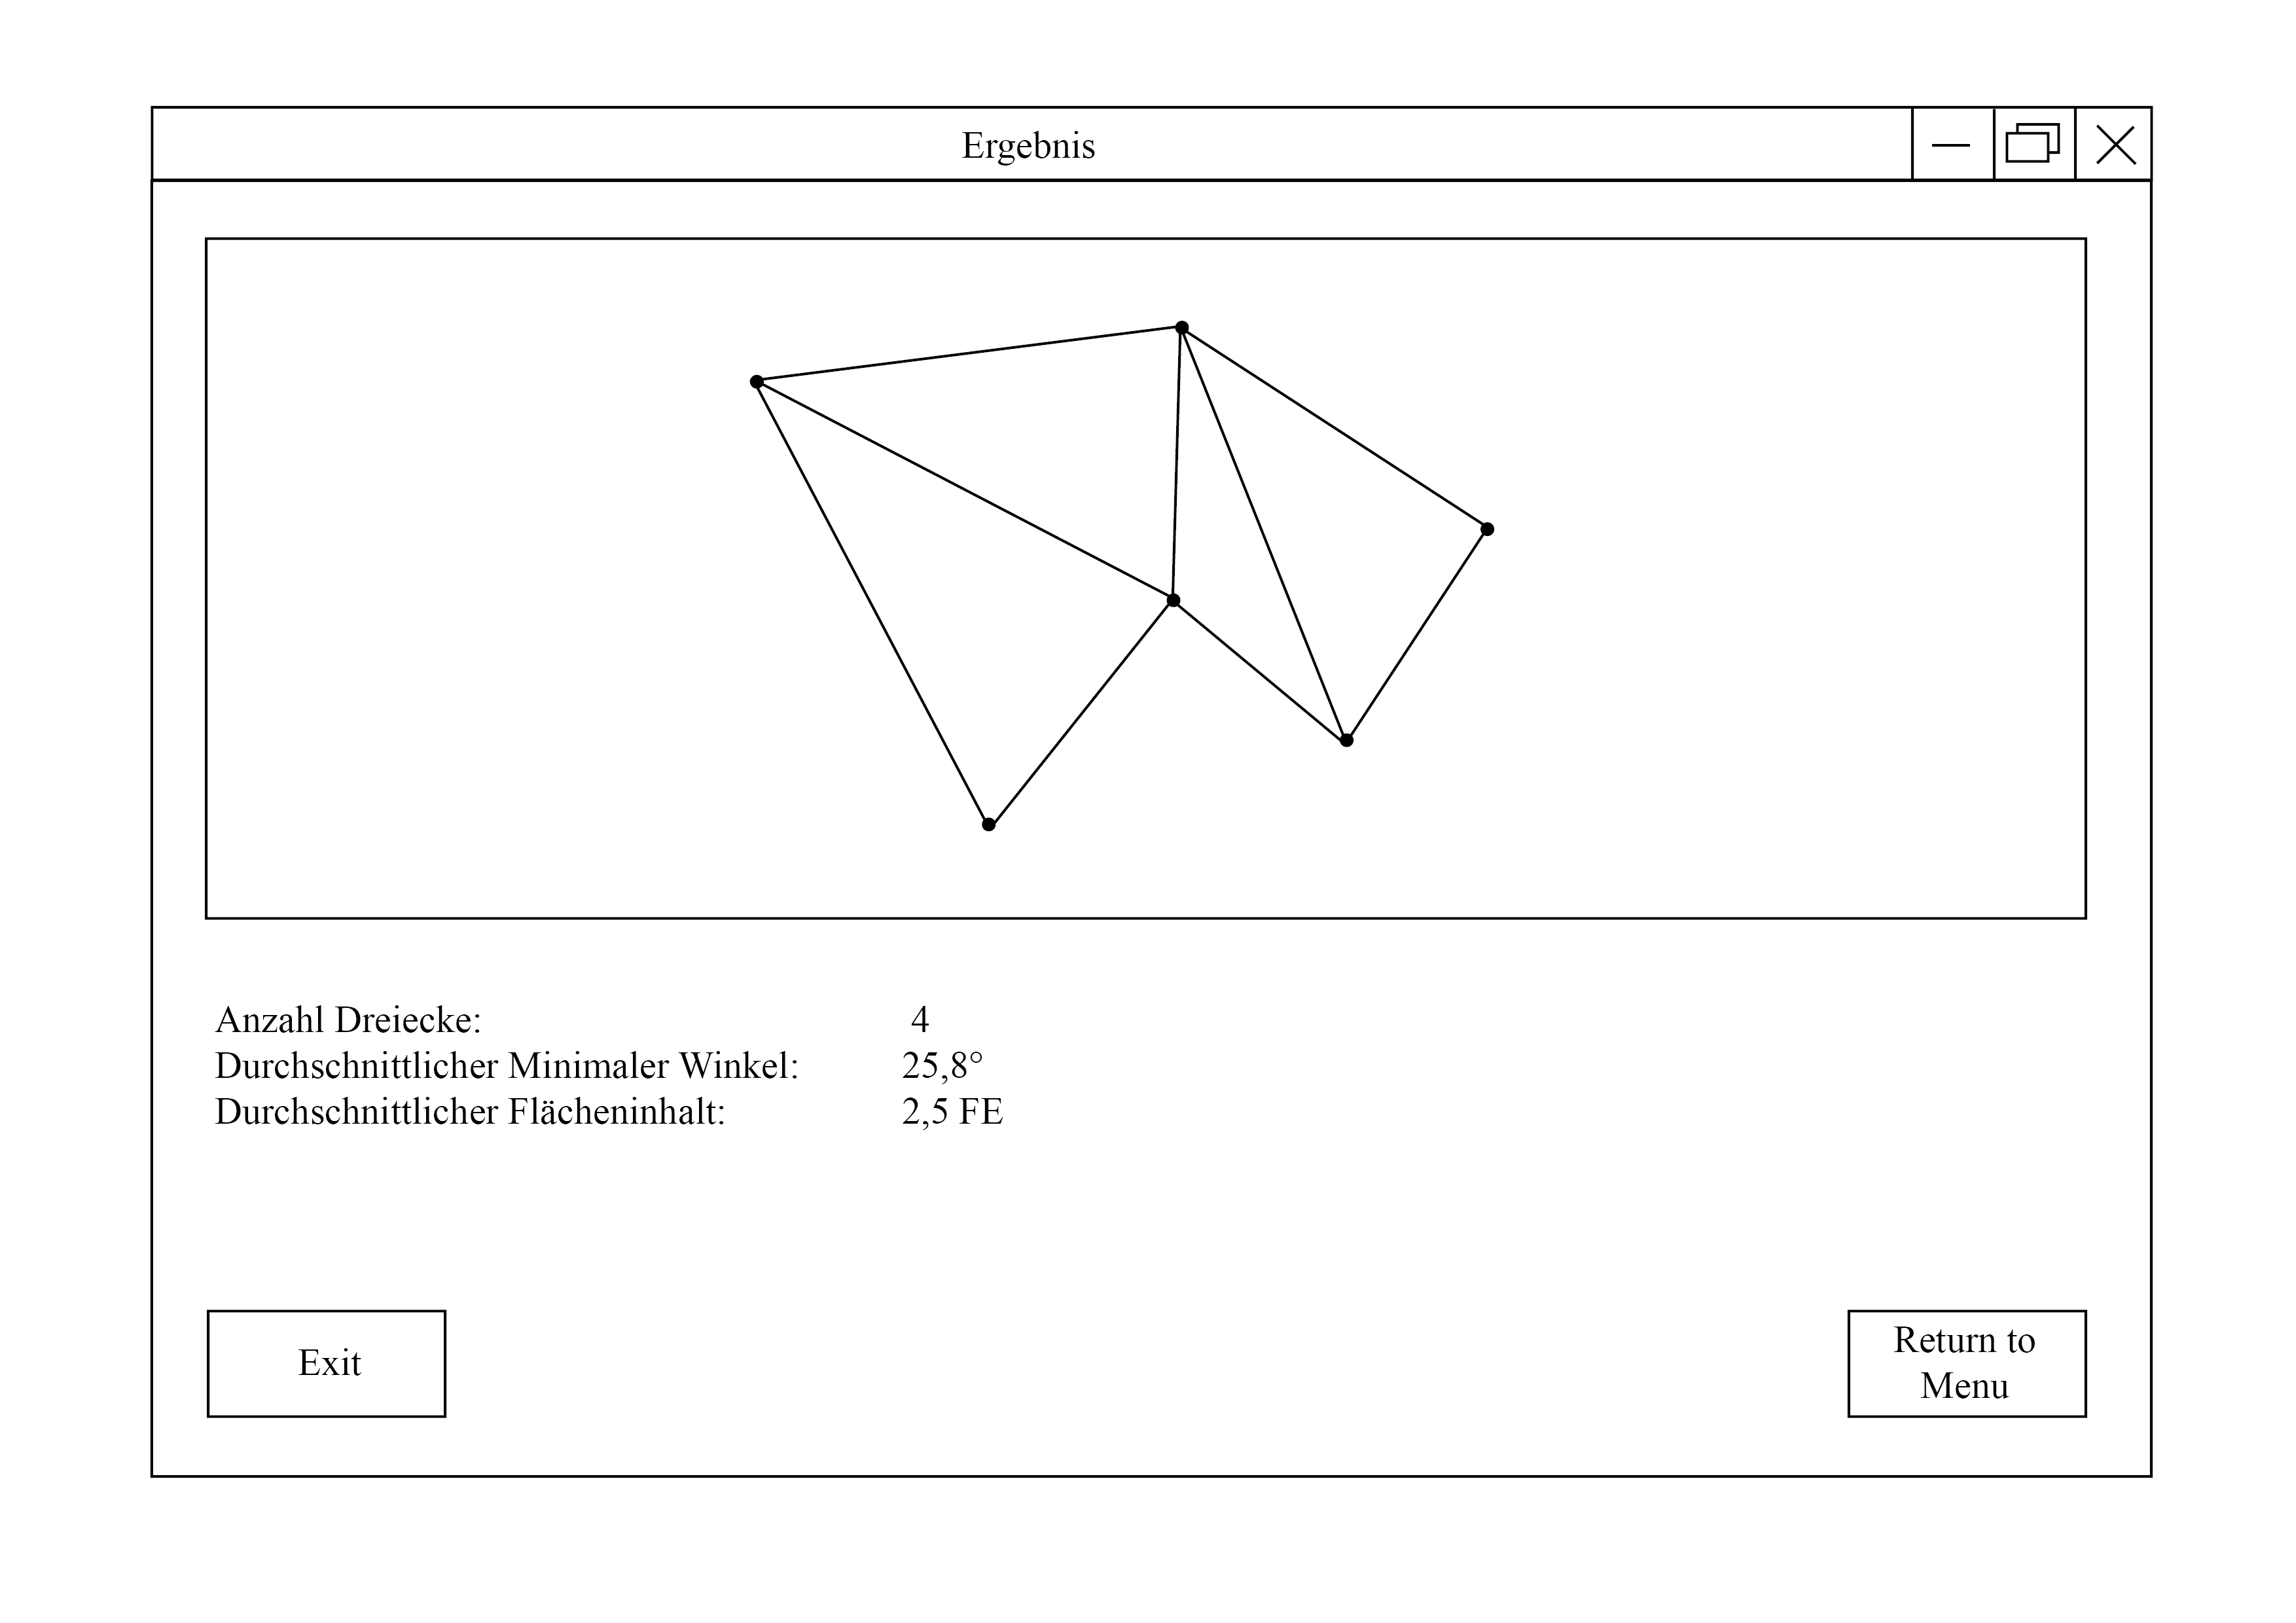
\includegraphics[width=1\textwidth]{bilder/ergebnis_metadaten.png}
    \caption[Entwurf Ergebnisseite mit Metadaten]{Ergebnisseite mit Ergebnisfenster und darunter Daten über das zerlegte Polygon}
    \label{fig:ergebnis_meta}
\end{figure}

\subsubsection{Resultat Entwurf - Vergleichsfenster}
Eine weitere Verbesserung der Ergebnisseite stellt dieser Entwurf dar. Zwar wurde der ursprüngliche Entwurf durch die Einführung der weiteren Informationen über das Polygon verbessert, jedoch fehlt immer noch eine Vergleichsmöglickeit.
Natürlich könnte der Nutzer mittels Bildschirmfoto und späterem Vergleich feststellen, welche seiner Einstellung die optimale Zerlegung herbeigeführt hat, jedoch ist das umständlich.
Um diesen Vergleich zu erleichtern, wird in diesem Entwurf ein zweites Anzeigefenster hinzugefügt. Dieses soll die perfekte Zerlegung des eingegebenen Polygons sowie seine Metadaten darstellen.
Damit kann der Nutzer feststellen, wie weit er vom Idealwert entfernt ist. Die übrigen Funktionen der Ergebnisseite werden aus dem vorangegangenen Entwurf übernommen.

\begin{figure}[h]
    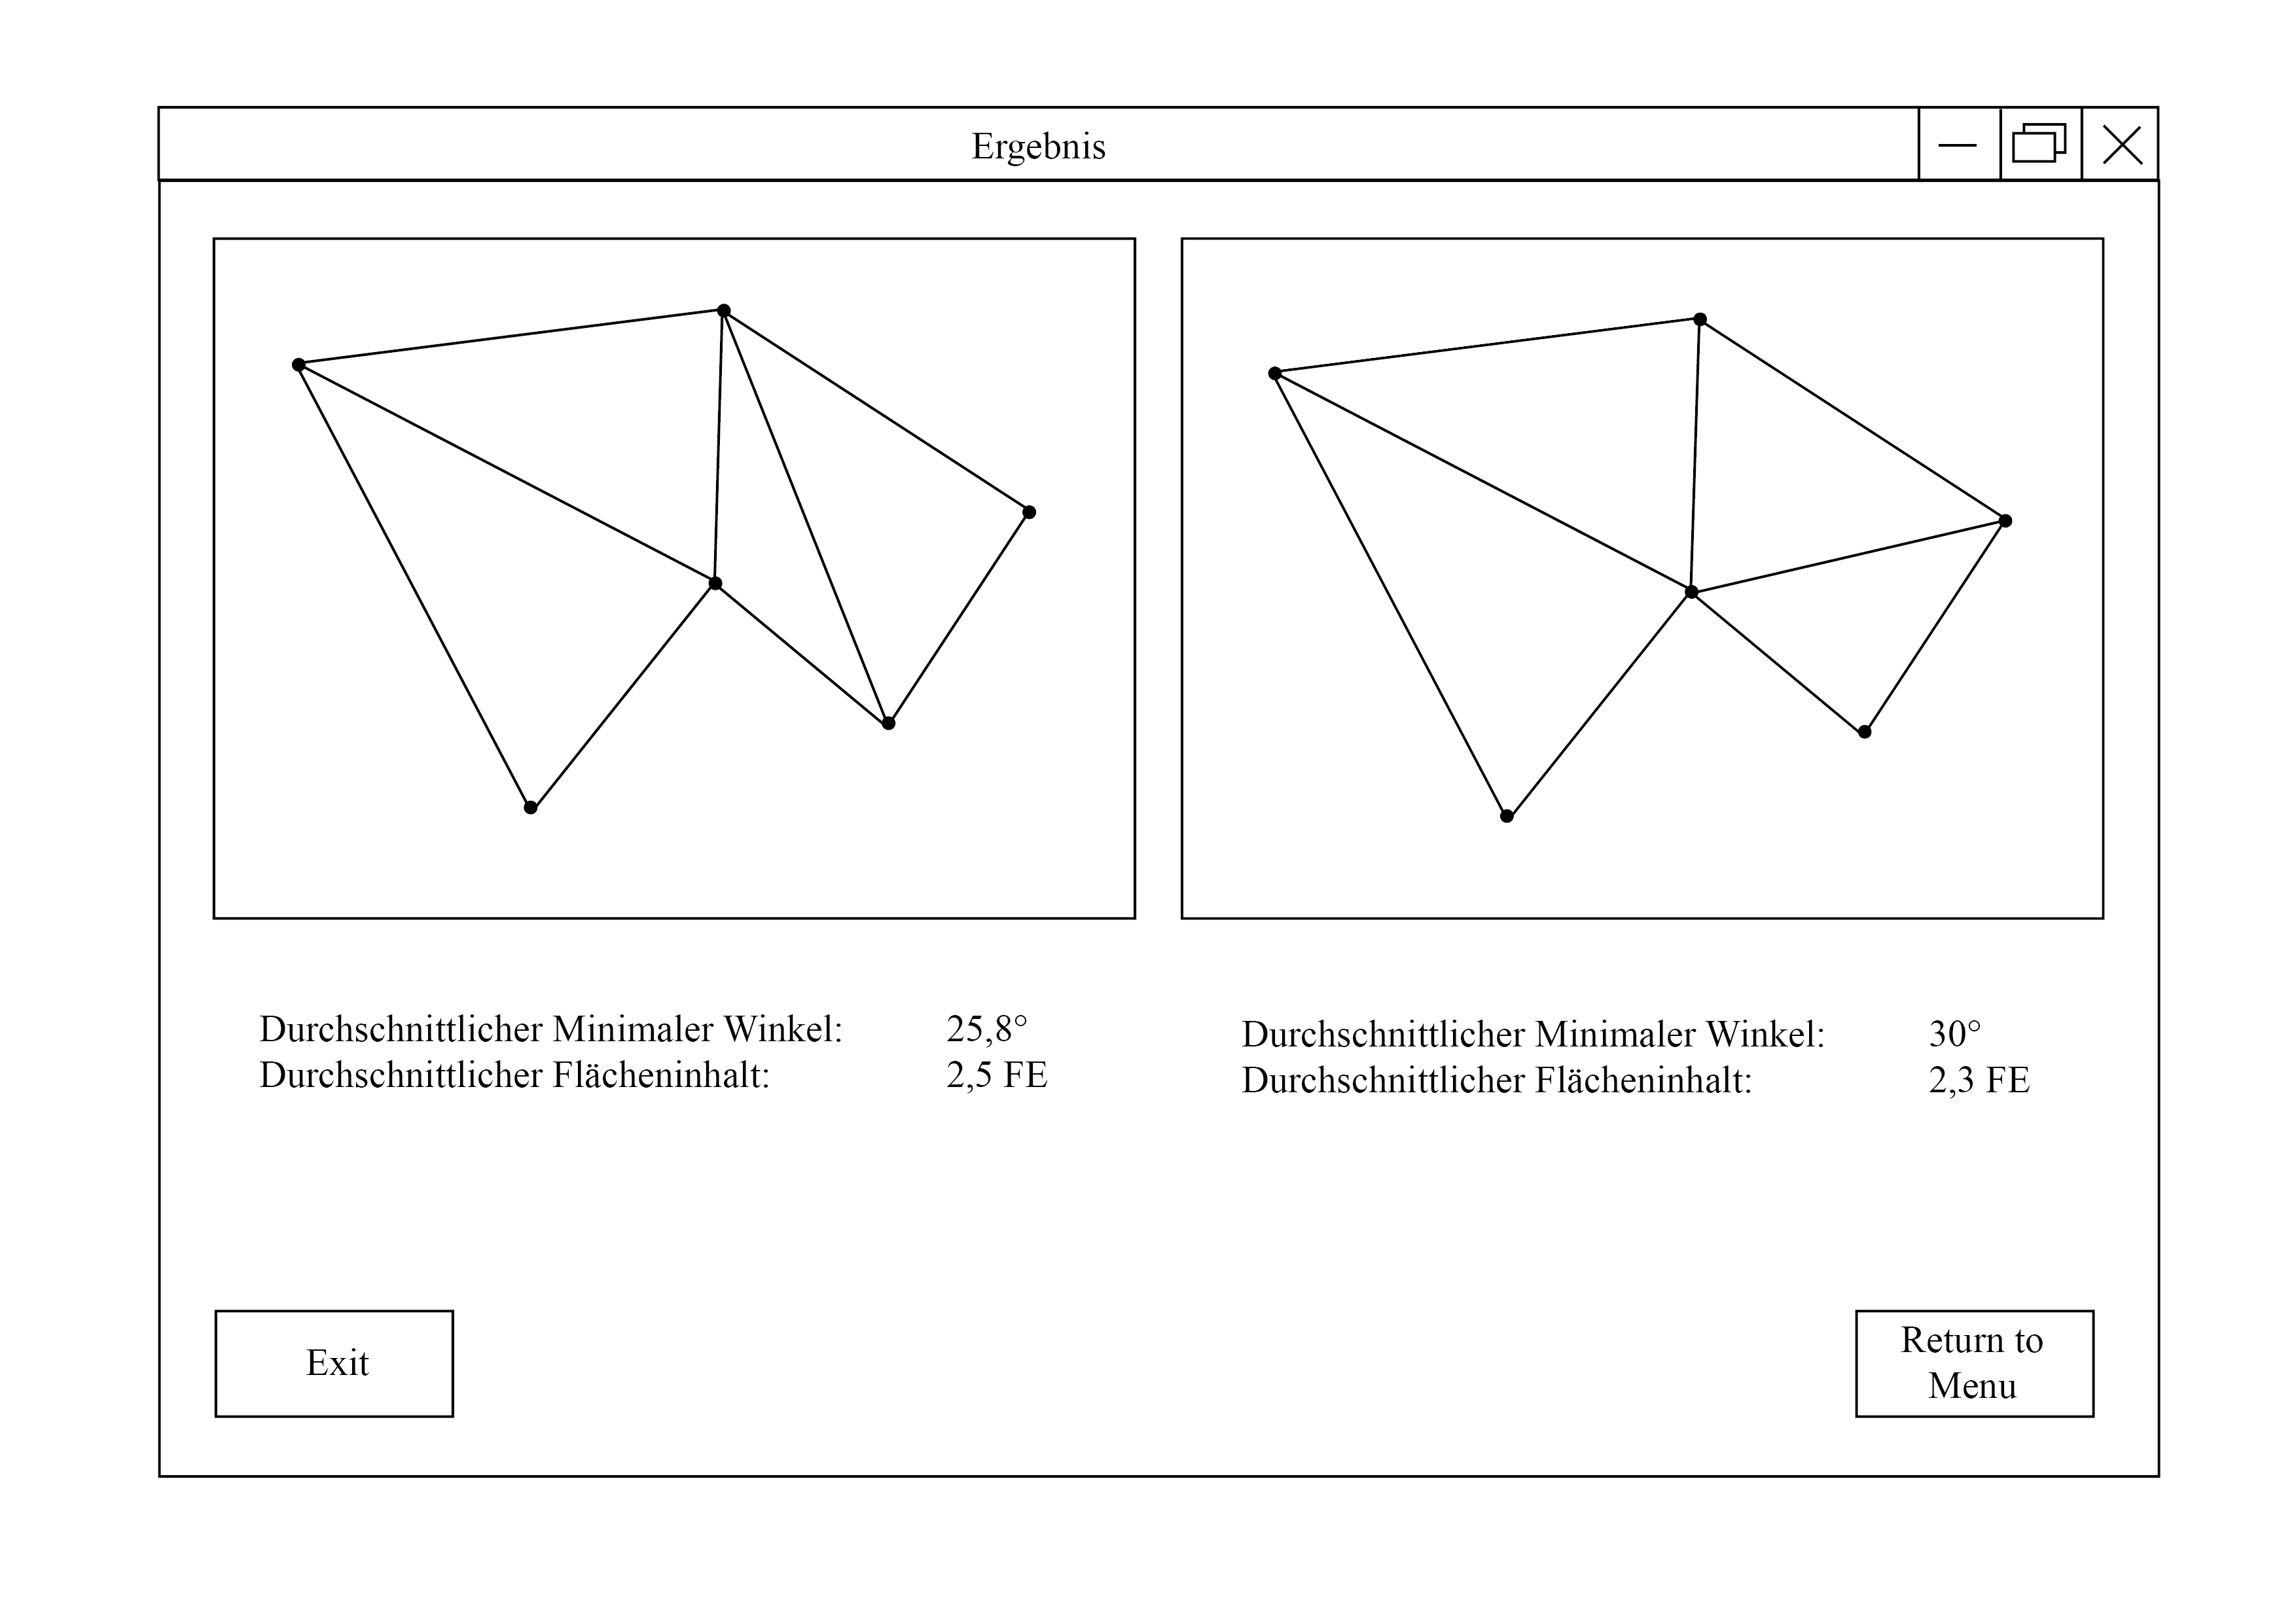
\includegraphics[width=1\textwidth]{bilder/ergebnis_vergleich.png}
    \caption[Entwurf Ergebnisseite mit Vergleichsfenster]{Ergebnisseite mit Vergleichsfenster, welches die optimale Zerleguzng des Polygons darstellt. Darunter Metadaten über die Zerlegungen.}
    \label{fig:ergebnis_vergleich}
\end{figure}

\subsubsection{Finalentwurf}
Der finale Entwurf setzt sich aus den besten oben angeführten Entwürfen zusammen. In Papierform umfasste er noch keine Farben oder ähnliches. Diese wurden erst in der eigentlichen Implementierung hinzugefügt, um das \ac{gui} noch weiter zu verbessern.
In seiner Gänze umfasst der Finalentwurf also das Menü, in welchem die Optionen inklusive sind, die Iterationsseite sowie die Ergebnisseite mit Vergleichsfenster. Die Übergänge zwischen den einzelnen Seiten wird wie in den jeweiligen Abschnitten beschriben geregelt.


\subsection{GUI und Pages}
Wie bereits in Kapitel 4.2.6 beschrieben, besteht das \ac{gui} aus drei Teilen. Diese werden durch einen Aufzählungstypen \lstinline{enum Page} dargestellt. Dieser besitzt drei Ausprägungen, wie im folgenden zu sehen, welche zusätzlich eigene Felder für die weitere 
Implementierung der Funktionalitäten besitzen. Dieses Struct wird in der \lstinline{main.rs} deklariert, sowie auch die anderen in diesem Abschnitt besprochenen Komponenten des Codes.

\begin{lstlisting}[language=C]
enum Page {
    Menu { 
        tools: Tools,
        progset: ProgramSettings,
        draw_panel: DrawPanel,
        confirm_button: button::State,
        undo_buffer: Vec<PageMessage>,
        action_buffer: Vec<PageMessage>,
        undo_performed: bool,
        dark_mode: bool,
    },
    Iteration {
        preview_panel: PreviewPanel,
        prevoius_button: button::State,
        next_button: button::State,
        end_button: button::State,
        dark_mode: bool,
        current_step: usize,
        
    },
    Result {
        result_panel: ResultPanel,
        repeat_button: button::State,
        exit_button: button::State,
        dark_mode: bool,
    },
}    
\end{lstlisting}

Auf jede dieser Ausprägungen wird in den folgenden Kapiteln gesondert eingegangen.
Als übergeordneten Datentyp existiert das \lstinline{struct Pages}. 
Es besitzt zwei Felder. Zum einen einen Vektor aus allen Seiten, welche Ausprägungen des \lstinline{enum Page} sind.
Zusätzlich gibt es noch den Zähler  \lstinline{current_page: usize} als Index für den eben beschriebenen Vektor. Er wird später verwendet, um
von einer Seite des Programms zur nächsten zu wechseln.

\begin{lstlisting}[language=C]
    struct Pages {
        pages: Vec<Page>,
        current_page: usize,
    }
\end{lstlisting}

Das \lstinline{struct Pages} erhält eine Implementierung mit verschiedenen Funktionen mit dem nachfolgenden Aufruf.
Die Funktionen sollen an dieser Stelle in vollständigem Umfang aufgeführt werden. Eine namentliche Erwähnung soll hier genügen. 
Nur auf die \lstinline{fn new()} soll einmal genauer eingegangen werden, damit sie exemplarisch für alle weiteren ähnlichen Funktionen erklärt wird.
Wichtig für die Funktionalität des Programms ist vor allem, dass \lstinline{current_page} mit \lstinline{0} initialisiert wird. Das ist gleichbedeutend mit dem Setzen der 
Startseite auf \lstinline{Page::Menu}.

\begin{lstlisting}[language=C]
    impl Pages {
        fn new() -> Pages { ... }
        fn update(&mut self, msg: PageMessage, ) { ... }
        fn view(&mut self) -> Element<PageMessage> { ... }
        fn advance(&mut self) { ... }
        fn return_to_menu(&mut self) { ... }
        fn can_continue(&self) -> bool { ... }
        fn title(&self) -> &str { ... }
    }
\end{lstlisting}

Mittels der \lstinline{fn new()} wird, bei einer Initialisierung einer Variable vom Typ \lstinline{Pages}, die Standardbelegung aller Felder dieses structs festgelegt. 
Dies geschieht beispielsweise beim Start des Programms. Die Datentypen, welche hier zugewiesen werden,
werden an anderer Stelle noch Erwähnung finden, wenn sie eine zentralere Rolle spielen.

Noch ist das Programm allerdings nicht lauffähig. Dazu fehlen noch drei wichtige Bestandteile. Als erstes das \lstinline{struct Gui}. Dieses umfasst zwei Felde, einmal 
\lstinline{pages: Pages} und \lstinline{dark_mod: bool}. Des weiteren wird für dieses Struct eine Implementierung einer \lstinline{iced::Sandbox} vorgenommen.
Die \lstinline{Sandbox} ist ein Applikationstyp aus der Iced-Bibliothek, welcher ein Programm mit \ac{gui} erzeugt, jedoch keine asynchronen Aktionen unterstützt. Hierfür müsste man
eine \lstinline{iced::Application} nutzen, was für einfache Anwendungen, wie diese Arbeit, nicht notwendig ist. Eine solche Implementierung sieht wie folgt aus:

\begin{lstlisting}[language=C]
    impl Sandbox for Gui {
        type Message = Message;

        fn new() -> Gui { ... }
        fn title(&self) -> String { ... }
        fn update(&mut self, event: Message) { ... }
        fn view(&mut self) -> Element<Message> { ... }
    }
\end{lstlisting}

Zuerst wird eine Typendefinition für \lstinline{Message} durchgeführt. Diese ist wichtig für zwei der vier obligatorischen Funktionen einer \lstinline{Sandbox}, denn 
mittels Nachrichten werden alle Rückmeldungen zu Nutzerinteraktionen abgebildet. Die \lstinline{fn new()} weißt den Feldern, wie bereits beschrieben, Standardwerte zu.

Die \lstinline{fn title(&self)} setzt den Text, welcher oben über einer Seite des Programms im Header angezeigt wird. Dieser wird je nach dem, welche Seite aktiv ist,
festgelegt. Dafür findet sich in der Implementierung \lstinline{impl Page} eine Funktion mit gleichem Namen. Diese ist nachfolgend abgebildet.

\begin{lstlisting}
  
    impl<'a> Page {
        
        fn title(&self) -> &str {
            match self {
                Page::Menu { .. } => 
                    "Triangulation for Polygons - Menu",
                Page::Iteration { .. } => 
                    "Triangulation for Polygons 
                        - Algorithm Iteration",
                Page::Result { .. } => 
                    "Triangulation for Polygons - Result",
            }
        }
    }

\end{lstlisting}

Die \lstinline{fn update(&mut self, event: Message)} hat die Aufgabe, die Übergänge zwischen den einzelnen Seiten zu bewerkstelligen und die jeweilige Update-Funktion 
der einzelnen Pages aufzurufen. Für die Übergänge werden bestimmte Nachrichten abgefangen, welche von Buttons auf den jeweiligen Seiten generiert werden. Dazu aber in späteren Kapiteln mehr.

Zu guter Letzt gibt es noch die \lstinline{fn view(&mut self)}. Diese ist für alle visuellen Aspekte des Programms zuständig. Hier wird das übergeordnete Layout der Pages festgelegt und die 
zur aktiven Page gehörende View-Funktion aufgerufen. Diese legt dann das spezielle Layout jeder Seite fest.

Die Nachrichten, welche während der Laufzeit des Programms von den einzelnen Interaktionselementen generiert und ausgegeben werden, müssen behandelt werden, um alle Funktionalitäten auch bei Aufruf auszuführen.
Dafür hat der der Struct \lstinline{Page} ebenfalls eine Funktion \lstinline{fn update()}. Diese besteht aus einem großen \lstinline{match}-Statement, welches für jeden auftretenden Nachrichtentypen vom Typ \lstinline{PageMessage} die gewünschten 
Aktionen durchführt. Dieses wird in späteren Kapiteln in Teilen betrachtet werden. Hier seinen einmal alle Nachrichtentypen angeführt. Diese sind in der Datei \lstinline{message.rs} definiert.

\begin{lstlisting}
    pub enum PageMessage {
        //Messegaes needed for inteactions on the menu page
        
        //Options
        AlgorithmSelected(Algorithm),
        HeuristicSelected(Heuristic),
        EdgeSwappingToggled(bool),
        StepTrigToggled(bool),
        DarkModeToggled(bool),
    
        //Drawing Tools
        DrawPressed,
        DrawHolePressed,
        UndoPressed,
        RedoPressed,
        ClearPressed, //Opens Popup
        PopUpClosed, //Closes PopUp
        AddPoint(Point),
        ConfirmPressed,
        ClearAll,
        RejectClear,
        
        //Messages for interactions on the iteration page
        PreviousPressed,
        NextPressed,
        EndPressed,
    
        //Messages for interactions on the result page
        ExitPressed,
        RepeatPressed,
    }
\end{lstlisting}

Das zweite noch fehlende Element, um das Programm lauffähig zu machen, ist die \lstinline{fn main()}. Diese ist das Kernstück eines jeden Rust-Programms. Sie ist so lange aktiv, bis das Programm beendet wird.
Sie hat in diesem Fall die Funktion, die \lstinline{Sandbox} zu starten und ablaufen zu lassen. Dazu können der \lstinline{fn Gui::run()}, welche durch die Implementierung der \lstinline{Sandbox} hinzugefügt wurde, verschiedene 
Einstellungsmöglichkeiten vom Typ \lstinline{Settings} übergeben werden. Darunter sind beispielsweise die Höhe und Breite des Programmfensters, ob dieses skalierbar sein soll und anderes. Alles was man nicht per Hand festlegt,
wird durch \lstinline{..Settings::default()} auf einen Standardwert gesetzt. Das Ganze sieht dann wie folgt aus: 

\begin{lstlisting}[language=C]
  
    pub fn main() -> iced::Result {

        Gui::run(Settings {
            antialiasing: true,
            window: window::Settings {
                resizable: false,
                position: Position::Centered,
                size: (1280, 720),
                ..window::Settings::default()
            },
            ..Settings::default()
        })
    }

\end{lstlisting}

Die letzte wichtige Komponente eines Rust-Projekts ist die \lstinline{Cargo.toml} Datei. Sie beinhaltet alle relevanten Informationen für den Compiler, wie zum Beispiel die 
Dependencies. Für dieses Projekt sieht es folgendermaßen aus:

\begin{lstlisting}
  
    [package]
        name = "src"
        version = "0.1.0"
        author = "Christoph Pooch"
        edition = "2021"

    [dependencies]
        iced = {version = "0.4", features = ["canvas"]}
        iced_aw = { version = "0.2", default-features = false, features = ["card"]}
        num-traits = "0.2"
    [[bin]]
        name = "src"
        path = "main.rs"

\end{lstlisting}

Das Programm kann nun mittels des Befehls \lstinline{cargo run} in der Kommandozeile ausgeführt werden.

\subsubsection{Page - Menu}
Wie bereits im Kapitel 4.2.6 zusehen war, setzt sich das Menü aus drei großen Bereichen zusammen, der Zeichenfläche, den Zeichenwerkzeugen und den Optionen. \linebreak

\textbf{Zeichenfläche}\linebreak
Über die Zeichenfläche, welche der zentralste Bestandteil des Menüs ist, wird das Polygon eingegeben, welches im weiteren Verlauf dann mittels des gewählten Algorithmus zerlegt werden soll.
Hierfür besitzt die \lstinline{Page::Menu} ein Feld \lstinline{draw_panel: DrawPanel}. Dieser Struct wird in der Datei \lstinline{draw_panel.rs} definiert und mehrere hat Felder, wie nachfolgend zu sehen. 
Davon ist \lstinline{polygon: DrawState} der Teil, welcher, zusammen mit dem Vektor \lstinline{vertices: Vec<Point>} als Eingabespeicher, die Zeichenfunktionalität umsetzt. Man kann sich den \lstinline{DrawState} als Zustandsautomaten 
vorstellen, welcher drei Zustände vom Typ \lstinline{pending: Option<Pending>} ( \lstinline{None, WaitNxtInput, ClipToStartVertex} ) und einen Cache für die Zeichenoperationen des Renderers besitzt. 

\begin{lstlisting}
    pub struct DrawPanel {
        pub polygon: DrawState,
        pub vertices: Vec<Point>,
        pub panel_width: u16,
        pub panel_height: u16,
        pub closed: bool,
        pub ignore_input: bool,}
\end{lstlisting}

Um nun einen Mausklick über dem Zeichenfenster abzufangen, wird vor jedem Zeichenvorgang eine Überprüfung durchgeführt, ob der Input gesperrt wurde. Das geschieht, wenn 
das Zeichenwerkzeug \emph{Draw} nicht aktiviert ist, damit keine ungewollten Eingaben entstehen. Wenn das nicht der Fall ist, also die Variable \lstinline{ignore_input: bool} auf \lstinline{false} gesetzt ist, dann 
wird eine zweite Überprüfung durchgeführt. Hierbei wird abgefragt, ob sich der Mauszeiger in den Grenzen des Zeichenfeldes befindet und eine relative Position bezogen auf das Zeichenfeldkoordinatensystem ausgegeben.

\begin{lstlisting}
    let cursor_position =
        if self.ignore_input {
            return (event::Status::Ignored, None);
        }
        else if let Some(position) = cursor.position_in(&bounds){
            position
        } else {
            return (event::Status::Ignored, None);
        };

\end{lstlisting}

Diese Information wird nun an den Zustandsautomat, der mittels einem \lstinline{match}-Statement umgesetzt wurde, übergeben. Er überprüft, ob ein Mausklick stattgefunden hat, und führt dann einen Zustandsübergang aus, wenn das geschehen ist.
Dabei wird bei Programmstart im Zustand \lstinline{None} begonnen. Nach der ersten Eingabe bleibt der Automat solange im Zustand \lstinline{WaitNxtInput} und gibt einen Nachricht vom Typ \lstinline{PageMessage::AddPoint(Point)} aus, bis sich der Mauszeiger in einem 
kleinen Bereich um den zuerst eingegebenen Eckpunkt des Polygons befindet. 
In diesem Fall geht er in den Zustand \lstinline{ClipToStartVertex} über. Hier wird kein Punkt hinzugefügt, sondern das Polygon mit einer letzten Kante geschlossen. Dazu wird die Variable \lstinline{closed: bool} des Zeichenfeldes auf \lstinline{true} 
gesetzt. 
Die angesprochene Nachricht wird, wie alle Nachrichten vom Typ \lstinline{PageMessage}, in der Funktion \lstinline{fn update()} des Structs \lstinline{Page} behandelt. Dies sieht folgendermaßen aus:

\begin{lstlisting}
    fn update(&mut self, msg: PageMessage) {
        match msg {
            PageMessage::AddPoint(vertex) => {
                if let Page::Menu { draw_panel, 
                    tools, action_buffer, undo_performed, 
                    undo_buffer,.. } = self {

                    tools.clear_active = true;
                    tools.undo_active = true;
                    
                    if *undo_performed {
                        undo_buffer.clear();
                        tools.redo_active = false;
                    }

                    Page::push_vertex_to_buffer(vertex, 
                        &mut draw_panel.vertices);            
                    
                    draw_panel.polygon.request_redraw();

                    action_buffer.push(
                        PageMessage::AddPoint(vertex));     
                }}
        ...
        }}
\end{lstlisting}
Es werden zunächst einmal zwei Buttons der nachfolgend besprochenen Zeichenwerkzeuge aktiviert - der \emph{Clear-} und der \emph{Undo-Button}. Dann wird eine Überprüfung durchgeführt, ob zuvor eine \emph{Undo-Aktion} 
durchgeführt wurde. Das wird später noch einmal thematisiert. Eben dafür wird auch die Nachricht selbst am Ende des Codeblocks noch in einen Buffer geschoben.
Die zentrale Aufgabe dieses Aufrufs ist jedoch das Hinzufügen des in der Nachricht angegebenen Punktes. Das geschieht mittels der Funktion \lstinline{fn push_vertex_to_buffer()}. Ihr wird 
der Punkt sowie der Buffer übergeben, in welchen er eingefügt werden soll. In diesem Fall ist es der Vektor \lstinline{draw_panel.vertices}. Danach wird noch der Cache des Renderers zurückgesetzt, wodurch alle Inhalte auf dem 
Zeichenfenster neu gezeichnet werden.\linebreak

\begin{figure}[h]
    \centering
    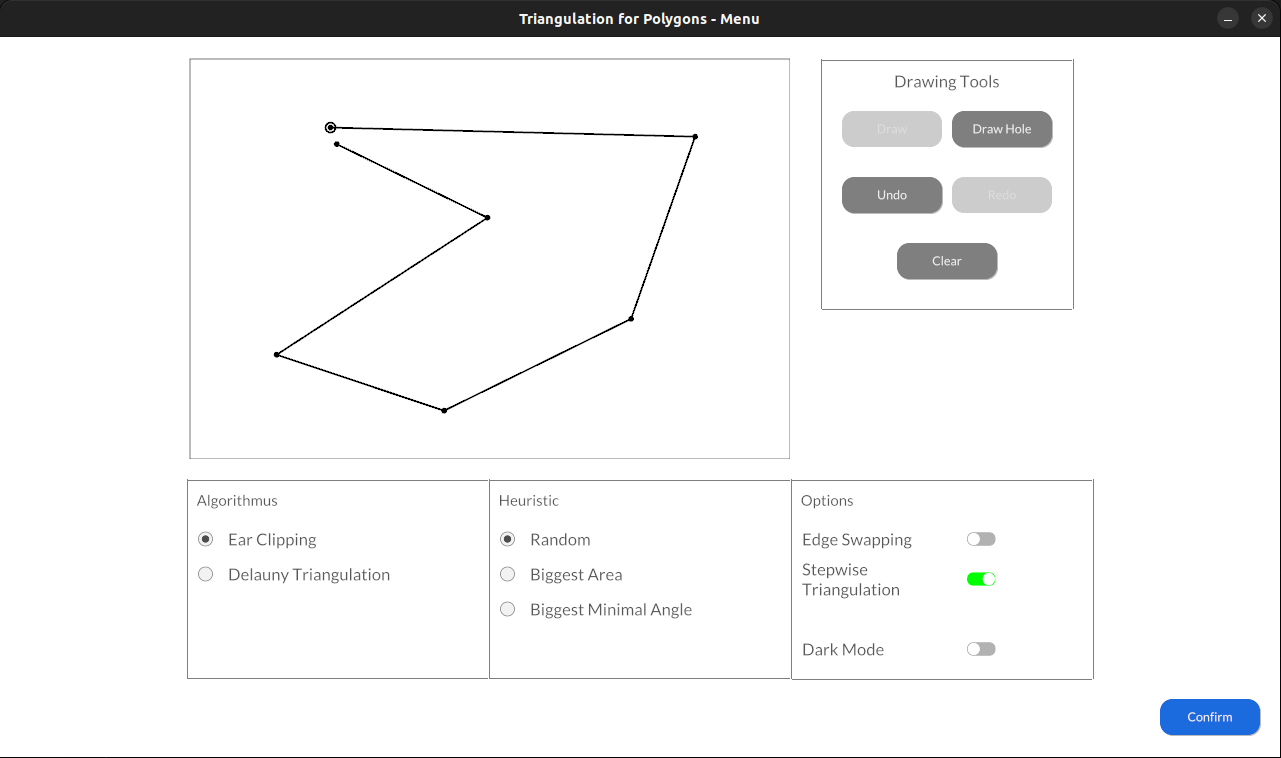
\includegraphics[width=0.8\textwidth]{bilder/menu.png}
    \caption[Menüseite der Anwendung]{Menüseite der Anwendung als Bildschirmfoto}
    
\end{figure}

\textbf{Zeichenwerkzeuge}\linebreak
Der zweite Bereich des Menüs, welcher eng mit dem Zeichenfenster verbunden ist, sind die Zeichenwerkzeuge. Dafür wurde ein neuer Struct in der Datei \lstinline{tools.rs} angelegt.  Bei den Zeichenwerkzeug handelt es sich im Wesentlichen um Buttons, welche verschiedene Funktionalitäten aktivieren.
Es gibt fünf solcher Buttons, welche jeder eine eigene Aufgabe erfüllen. Namentlich sind das der \emph{Draw-}, der \emph{Draw Hole-}, der \emph{Undo-}, der \emph{Redo-} und der \emph{Clear-}Button. Auf jeden davon wird im folgenden einmal gesondert eingegangen.
Der Tool-Struct umfasst also die Zustände der Buttons sowie einigen Boolean-Variablen, welche angeben, ob ein Button aktiv ist oder nicht. Des weiteren umfasst die Implementierung dieses Structs die Funktion \lstinline{pub fn tool_menu()}, welche das Layout der Zeichenwerkzeuge festlegt.
Zu besseren Übersicht für den Nutzer wurden diese fünf Buttons in einer umrahmten Gruppe rechts vom Zeichenfeld angeordnet.

Bevor nun auf die einzelnen Buttons und deren Funktionalität eingegangen wird, soll hier kurz beschrieben sein, wie ein \lstinline{iced::button} überhaupt aufgebaut ist. 
Wie angedeutet, ist ein Button ein Element aus der Iced-Bibliothek. Es besitzt einen Zustand und ein Label, also eine Beschriftung. Zusätzlich gibt es noch eine Nachricht, welche beim Drücken des Buttons ausgelöst wird, und neben vielen weiteren Einstellungen wie Breite und Höhe auch noch einen 
Stil, welcher mittels eines \lstinline{StyleSheets} festgelegt werden kann. Eine Nachricht wird durch den Befehl \lstinline{mybutton.on_press(Message)} an den Button gebunden. 
Zu Stilen ist im Kapitel 4.3.4 mehr beschrieben. Hier einmal der grundsätzliche Aufruf eines neuen Buttons:


\begin{lstlisting}
    use iced::{Button, button, Text};
    neuer_button = Button::new(button::State::new(), 
                   Text::new("Beschriftung"))
                   .on_press(Message).style(ButtonStyle);
\end{lstlisting}

Das Layout, welches in der Funktion \lstinline{pub fn tool_menu()} festgelegt wurde, ist im nachfolgenden Bild noch einmal als Ausschnitt aus dem vollständigen Menü zusehen.
\linebreak

\textbf{\small{Draw-Button}}\linebreak
Dieser Button hat eine der wichtigsten Funktionen des Programms. Er aktiviert die Eingabe auf dem Zeichenfeld. Standardmäßig ist er aktiv, das heißt, es ist möglich ihn zu drücken. Einmal gedrückt, wird er so lange 
deaktiviert, bis ein anderer Button gedrückt wurde. Während er inaktiv ist, das heiß er gedrückt wurde, kann man nach belieben auf dem Zeichenfeld ein Polygon durch Mausklicks erzeugen. Ist dieses dann geschlossen, wird der 
Input wieder deaktiviert.\linebreak

\textbf{\small{Draw-Hole-Button}}\linebreak
Der \emph{Draw-Hole-Button} soll, wie der \emph{Draw-Button}, den Input auf dem Zeichenfeld erlauben. Anders als bei \emph{Draw} soll hier aber nicht auf dem ganzen Zeichenfeld
gezeichnet werden, sondern nur innerhalb des zuvor gezeichneten Polygons. Es sollen also Löcher zum Polygon hinzugefügt werden. Dies ist zum Zeitpunkt der Abgabe dieser Arbeit noch nicht implementiert, wird aber später hinzugefügt.
%evtl rausstreichen
\linebreak

\textbf{\small{Undo-Button}}\linebreak
Das Rückgängigmachen von Aktionen ist ein wichtiger Aspekt, wenn es um Nutzerfreundlichkeit geht. Daher wurde diese Funktion mittels des \emph{Undo-Buttons} implementiert.
Er wird erst aktiv, wenn bereits mindestens ein Punkt auf dem Zeichenfeld gezeichnet wurde. Wird er gedrückt, so wir der zuletzt gezeichnete Eckpunkt aus dem Vektor \lstinline{draw_panel.vertices}, sowie die Nachricht \lstinline{AddPoint(Point)}
aus dem \lstinline{action_buffer} entfernt. In einen zweiten Buffer, den Vektor \lstinline{undo_buffer}, wird dann eine Kopie dieser entfernten Nachricht eingefügt. Sie enthält auch den gelöschten Punkt.
Dies geschieht, damit er mittels des \emph{Redo-Buttons} wieder hinzugefügt werden kann. Dazu im nachfolgenden Abschnitt mehr. Das Drücken des \emph{Undo-Buttons} löst die Nachricht 
\lstinline{PageMessage::UndoPressed} aus, welche dann in der Funktion \lstinline{fn update()} des Page-Struct behandelt wird. Sollte das Polygon zuvor geschlossen worden sein, dann muss dieser Zustand natürlich wieder aufgehoben werden und der Zustand 
des Zeichenautomaten \lstinline{DarwState} muss wieder auf \lstinline{Pending::WaitNxtInput} gesetzt werden. All das wird in der Update-Funktion umgesetzt. Auch wird eine Flag gesetzt, dass die zuletzt durchgeführte Aktion ein Rückgängigmachen war. Das wir 
für die Redo-Aktion relevant.\linebreak

\textbf{\small{Redo-Button}}\linebreak
Der \emph{Redo-Button} stellt das logische Gegenstück zum \emph{Undo-Button} dar. Aktionen, welche mittels Undo rückgängig gemacht wurden, können hiermit erneut durchgeführt werden. Auch dieser Askept ist für die Nutzerfreundlichkeit sehr wichtig.
Zunächst einmal ist dieser Button aber inaktiv. Erst wenn eine Undo-Aktion durchgeführt wurde, kann der \emph{Redo-Button} gedrückt werden.
Wird der \emph{Redo-Button} betätigt, löst er die Nachricht \lstinline{PageMessage::RedoPressed} aus. Diese führt in der \lstinline{fn update()} des Page-Structs zu verschiedenen Abläufen.
Als erstes wird die letzte Nachricht aus dem \lstinline{undo_buffer} entfernt und wieder in den \lstinline{action_buffer} geschrieben. Der zuvor entfernte Punkt, wird wieder in den dafür vorgesehenen Speicher eingefügt.
Sollte es noch weitere Aktionen geben, welche rückgängig gemacht wurden, dann bleibt der Button aktiv und kann erneut gedrückt werden.

In einem weiteren Fall, außer dem, dass der \lstinline{undo_buffer} leer ist, wird der Button auch deaktiviert. Im Prinzip liegt das auch daran, dass der \lstinline{undo_buffer} geleert wurde, aber auf andere Art.
Das geschieht, wenn nach einem Undo ein Draw passiert ist. Zuvor wurde bei der Undo-Aktion eine Flag gesetzt, welche anzeigt, dass die letzte Aktion rückgängig gemacht wurde. Wird jetzt ein neuer Eckpunkt gezeichnet, 
dann wird der \lstinline{undo_buffer} gelöscht. Das geschieht, damit keinen Punkte, welche gelöscht wurden an falscher Stelle wieder in den Vertex-Buffer eingefügt wird. Im nachfolgenden Bild ist das einmal aufgezeigt.
%Bild falscher Redo
\pagebreak

\begin{figure}[t]
    \centering
    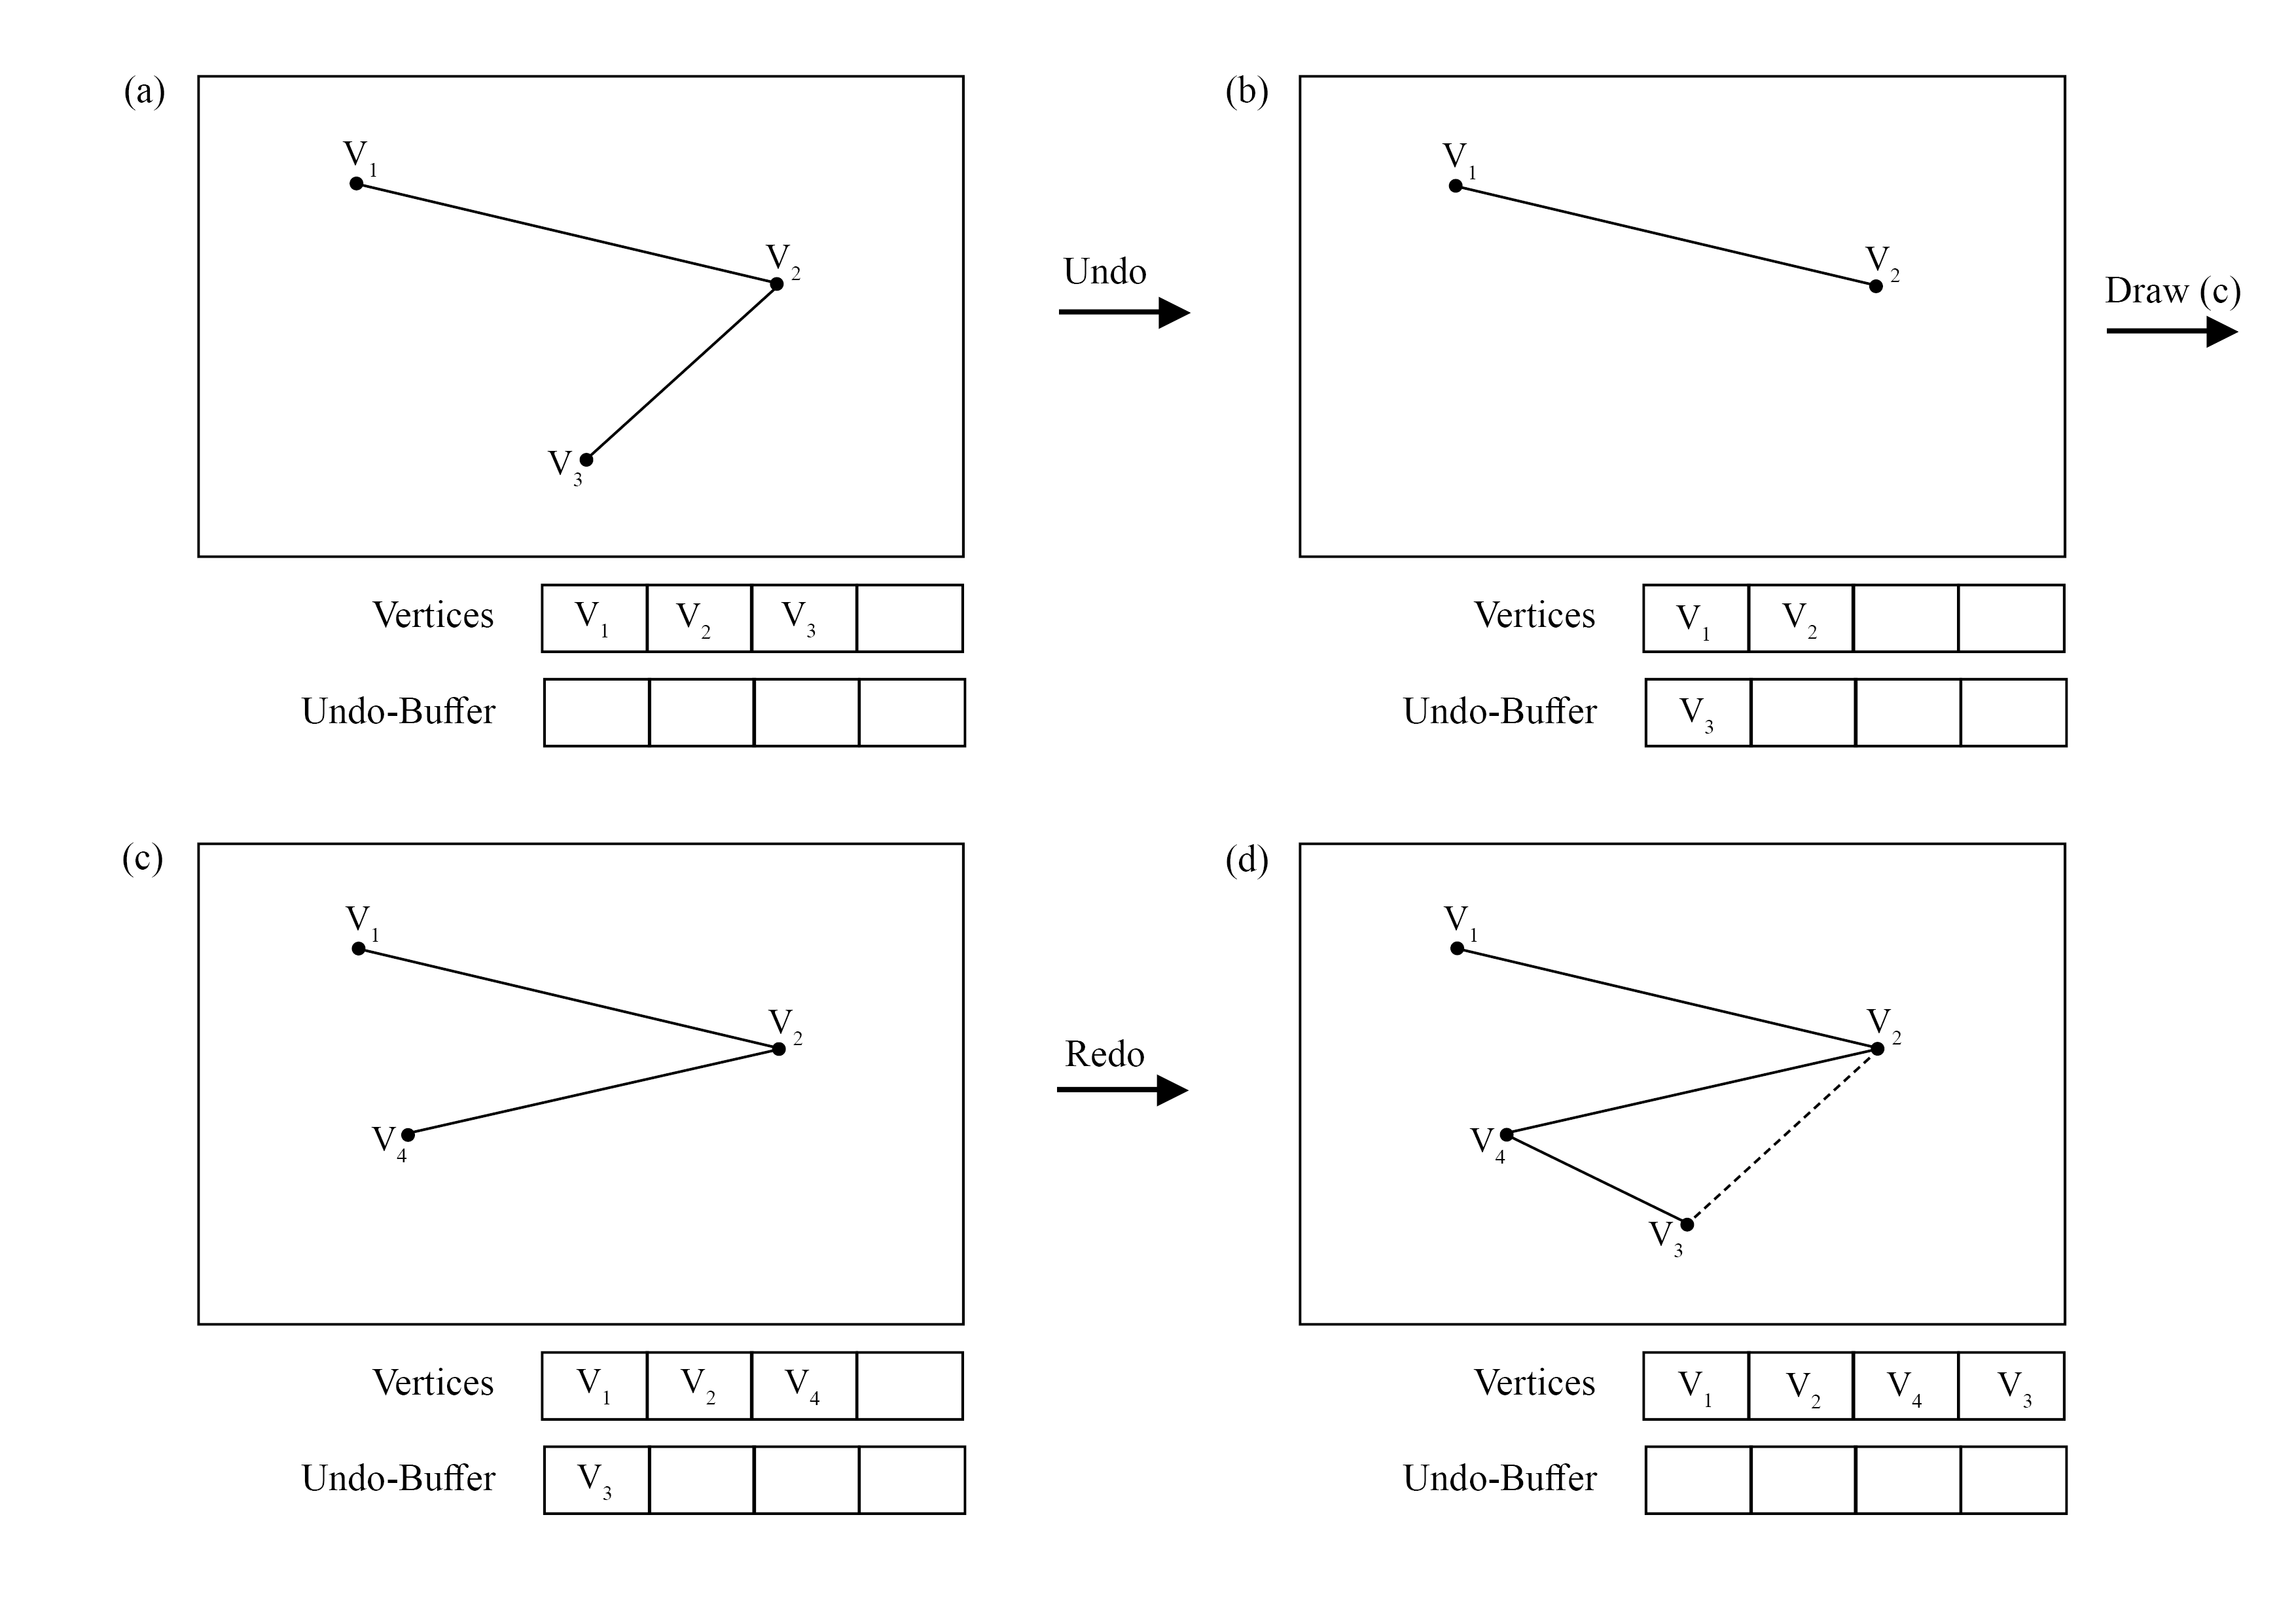
\includegraphics[width=0.7\textwidth]{bilder/falseRedo.png}
    \caption[Fehlerhafter Redo-Vorgang]{Fehlerhafter Redo-Vorgang. Punkt $v_3$ wird entfernt, dann $v_4$ hinzugefügt und später $v_3$ wiederhergestellt.}
\end{figure}
\textbf{\small{Clear-Button}}\linebreak
Dieser Button bildet eine Ausnahme unter den Zeichenwerkzeugen, da seine Funktion eine extra Bestätigung durch ein Dialogfenster benötigt, welches sich dann öffnet, wenn dieser Button gedrückt wurde. 
Dieses Dialogfenster ist kein Element der Iced-Bibliothek. Es gehört zur Bibliothek \lstinline{iced_aw}, welche eine Erweiterung von \lstinline{iced} darstellt und weitere weniger grundlegende \ac{gui}-Elemente umfasst.

\begin{wrapfigure}{h}{0.33\textwidth}
    \centering
    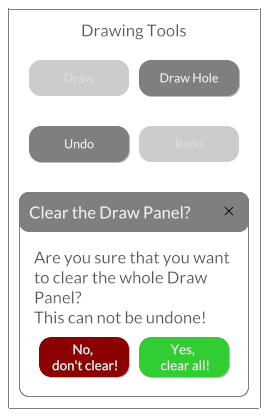
\includegraphics[width=0.3\textwidth]{bilder/clear_dialog.png}
    \caption[Clear-Dialogfenster]{offenes Clear-Diaglogfenster auf der Menüseite}
\end{wrapfigure}

Das verwendete Element ist eine \lstinline{iced_aw::Card}, welche man sich als Fenster im Fenster vorstellen kann. Sie besteht aus Header, Body und Footer und sendet beim Schließen eine Nachricht. 
Im Falle dieser Arbeit ist das \lstinline{PageMessage::PopUpClosed}. Der Body der Karte enthält dabei die Warnung, dass nach der Bestätigung des Löschungsvorganges der gesamte Input auf dem Zeichenfenster gelöscht wird und dies nicht rückgängig gemacht werden kann.
Diese Entscheidung wird mittels eines roten und eines grünen Buttons getroffen. Der rote \emph{Reject-Button} sendet dabei die Nachricht \lstinline{PageMessage::RejectClear} und setzt damit die gleiche Funktionalität um wie die Nachricht \lstinline{PageMessage::PopUpClosed}.
Mit dem grünen \emph{Yes-Clear-Button} wird die Löschung mittels der Nachricht \lstinline{PageMessage::ClearAll} ausgelöst. Beide Buttons schließen die Karte mit dem Dialog und lassen den Ursprünglichen \emph{Clear-Button} wieder erscheinen. 
\linebreak 

\textbf{\large{Optionen}}\linebreak
Der dritte und letzte große Bestandteil der Menü-Seite sind die Optionen. Diese sind ebenfalls noch einmal in drei Teile geteilt, welche optisch, wie auch die Zeichenwerkzeuge, durch einen Rahmen 
abgegrenzt werden. Bei den drei Sektionen handelt es sich um die Auswahl des Algorithmus, die Auswahl der anzuwendenden Heuristik und die weiteren Optionen.
In den ersten beiden Bereichen werden die Auswahlmöglichkeiten durch eine Selektion mittels Radio Buttons abgebildet. Ein Radio Button bzw. eine Radio Button Gruppe hat die Eigenschaft, dass nur eine Option zur gleichen Zeit aktiv sein kann.
Das bedeutet, wenn es drei Möglichkeiten (a), (b) und (c) gibt, dann kann man nur eine der drei, zum Beispiel (b), nicht aber zwei verschiedene, wie etwa (a) und (c), gleichzeitig auswählen.
Die Iced-Bibliothek besitzt eine Implementierung für eben solche Radio Buttons. Man kann sie automatisch aus einem Aufzählungstypen generieren, wenn man für diesen eine Implementierung für \lstinline{impl From<Algorithm> for String} und eine Funktion 
\lstinline{fn all()} bereitstellt. Die Funktion gibt schlichtweg alle Ausprägungen des Aufzählungstypen aus. Die String-Implementierung generiert aus einer gegebenen solchen Ausprägung eine Zeichenkette.
Anhand der Algorithmus-Auswahl sieht das dann in etwa so aus:

\begin{lstlisting}

    pub enum Algorithm {
        EarClipping,
        DelaunyTriangulation,}

    impl<'a> Algorithm {
        pub fn all() -> [Algorithm; 2] {
            [Algorithm::EarClipping,
             Algorithm::DelaunyTriangulation,]
        }}

    impl From<Algorithm> for String {
        fn from(algorithm: Algorithm) -> String {
            String::from(match algorithm {
                Algorithm::EarClipping => "Ear Clipping",
                Algorithm::DelaunyTriangulation => 
                    "Delauny Triangulation",
            })
        }}
\end{lstlisting}
Man bemerke, dass hier zu Beispielzwecken die \ac{dt} als Option aufgeführt ist. Diese ist in der beiliegenden Version des Programms nicht anwählbar. Sie 
ist als Idee der Programmerweiterung im Ausblick noch einmal angeführt.
Die Umsetzung einer automatischen Generierung der Radio Buttons würde dann in etwa so aussehen:

\begin{lstlisting}
    Algorithm::all().iter().cloned().fold(
        Column::new().padding(10).spacing(15),
        |choices, algorithm| {
            choices.push(Radio::new(
                algorithm,
                algorithm,
                selection,
                PageMessage::AlgorithmSelected,
            ).text_size(20).size(15))
        },
    )
\end{lstlisting}

Wie für die Algorithmen in der Datei \lstinline{algorithm.rs} wird nach dem gleichen Schema die selbe Implementierung für die Heuristiken in der Datei \lstinline{heuristc.rs} vorgenommen.
In der Datei \lstinline{program_settings.rs} wir nun der \lstinline{struct ProgramSettings} deklariert, welcher neben  \lstinline{algorithm: Option<Algorithm>} und \lstinline{heuristic: Option<Heuristic>}
auch \lstinline{bools: ProgramSettingsBools} beinhaltet. Dieses Feld umfasst die weiteren Optionen, welche man wahlweise aus- oder anschalten kann. In der finalen Version der Software sind dies zwei Möglichkeiten.
Die Option \emph{Stepwise Triangulation} für die Auswahl, ob der Algorithmus in Schritten oder im Ganzen ausgeführt werden soll, und die Option für den Dark Mode, welcher in Kapitel 4.3.4 beschrieben wird.
Diese Optionen werden durch sogenannte Toggler abgebildet. Ein Toggler hat neben einer Beschriftung auf eine Variable vom Typ Boolean, welchen er je nach seiner eigenen Stellung auf \emph{ein} oder \emph{aus} auf 
\lstinline{true} oder \lstinline{false} setzt. Anhand der Option des Dark Modes sieht das dann so aus:

\begin{lstlisting}
    Toggler::new(
        bools.dark_mode,
        String::from("Dark Mode"),
        PageMessage::DarkModeToggled,
    ).size(15).text_size(20)
\end{lstlisting}\pagebreak

\textbf{\large{Seitenübergang}}\linebreak
Zusetztlich zu den drei großen Bereichen des Menüs gibt es noch ein weiteres Interaktionselement. Dies ist ein Button, welcher unter den Optionen am rechten Rand des Fensters platziert wurde.
Das ist der \emph{Confirm-Button}. Dieser ist, im Gegensatz zu den Zeichenwerkzeugen kein Button mit Sekundärstil sondern ein Primärbutton. Er betsätigt nämlich alle Einstellungen und Eingaben der Menüseite und
regelt den Übergang auf die Iterationsseite. Dazu wird die Nachricht \lstinline{PageMessage::ConfirmPressed} gesendet. Damit das eingegebene Polygon auch auf der nächsten wie auch letzten Seite angezeigt wird, gibt es im Page-Struct
mehrere Funktionen, welche aufgerufen werden, sobald ein Seitenübergang stattfindet. Zuerst einmal muss der Speicher, welcher alle eingegebenen Eckpunkte beinhaltet, ausgelesen werden. Dies geschieht mittels der Funktion 
\lstinline{fn get_vertex_buffer(&mut self)}. Wurde der Buffer ausgelesen, dann muss er in das Koordinatensystem des Anzeigefensters der nächsten Seite konvertiert werden. Das ist notwendig, da alle Anzeigefenster unterschiedliche Größen besitzen.
Das bewerkstelligt die Funktion \lstinline{fn buffer_move_center(buffer: Vec<Point>, offset_x: f32, offset_y: f32)}. Sie erhält als Eingaben neben dem Buffer auch den jeweiligen Offset in x- und y-Richtung
zwischen den beiden Koordinatensystemen. Ist die Transformation geschehen, wird der Buffer mittels der Funktion \lstinline{fn set_vertex_buffer(&mut self, buffer: Vec<Point>)} auf die nächste Seite kopiert.

Für den Übergang zwischen Menü und Iteration genügt das. Für den später noch folgenden Übergang zwischen Iteration und Resultatsseite muss zusätzlich noch der Speicher für die erzeugten Diagonalen übergeben werden.
Dies geschieht nur mittels Kopiervorgang, da keine Koordinaten, sondern Anfangs- und Endpunkte der Strecken gespeichert wurden.

\subsubsection{Page - Iteration}

Die zweite Seite und das eigentliche Kernstück des Programms ist die Iterationsseite. Auf ihr spielt sich die gesamte Visualisierung des algorithmischen Ablaufs ab.
Sie besteht aus nur zwei Teilen. Dem Vorschaufenster und der Navigationsleiste. Den Großteil der Bildfläche nimmt dabei eben jenes Vorschaufenster ein, auf dem das im Menü eingegebene 
Polygon zu sehen ist. Hier werden auch die vom Algorithmus ermittelten Diagonalen eingezeichnet, welche die Triangulation bilden. Diese Einzeichnen geschieht schrittweise, sofern 
im Menü die Option \emph{Stepwise Triangulation} auf aktiv gesetzt wurde. Anderenfalls wird die Iterationsseite übersprungen und sofort die Ergebnisseite aufgerufen.

Das Vorschaufenster wird in der Datei \lstinline{preview.rs} definiert und ist eine vereinfachte Form des Zeichenfensters. Hier ist allerdings die Eingabe standardmäßig deaktiviert, da vom Benutzer keine 
Auswahlen erwartet werden. Nur wenn die Heuristik \emph{Manual Selection} im Menü gewählt wurde, kann der Benutzer per Klick auf ein Dreieck den nächsten Triangulationsschritt bestimmen.
In allen anderen Fällen wird das Dreieck, welches mittels einer Diagonalen gebildet werden soll, automatisch anhand der gewählten Heuristik ausgewählt.

Von einem zum nächsten Iterationsschritt gelangt der Nutzer über einen Button in der Navigationsleiste. Der \emph{Next-Button} erhöhrt den Zähler, welcher den Fortschritt der Triangulation anzeigt, 
und lässt die Anzeige um die neu erzeugte Diagonale erweitern. Es handelt sich hierbei um einen Primärbutton, der dem Nutzer suggerieren soll, dass dies der empfohlene Weg ist, um durch die Triangulation zu navigieren.

Um sich vergangene Iterationsschritte erneut anzegen zu lassen, gibt es den \emph{Previous-Button}, dieser senkt den Fortschrittszähler und zeigt den vorherigen Iterationsschritt auf dem Vorschaufenster an.
Dabei kann man allerdings nicht weiter als bis zum ersten Schritt zurückkehren, da der Button dann deaktiviert wird. Es gibt also keine Möglichkeit, um von der Iterationsseite direkt zur Menüseite zurückzukehren.
Damit das Anzeigen vergangener Schritte nicht als Pflicht empfunden wird, ist der \emph{Previous-Button} im Sekundärstil gehalten.

Hat der Algorithmus alle Schritte durchlaufen, dann wird aus dem \emph{Next-Button} der \emph{End-Button}. Dieser kopiert den Vertex-Buffer wie auch den Diagonalen-Buffer von der Iterationsseite auf die Ergebnisseite 
und sendet die Nachricht \lstinline{PageMessage::EndPressed}, welche von der Update-Funktion des Pages-Structs als Signal zum Übergang auf die Ergebnisseite interpretiert wird. Der \emph{End-Button} ist ebenso wie der 
\emph{Next-Button} ein Primärbutton.

\begin{figure}[h]
    \centering
    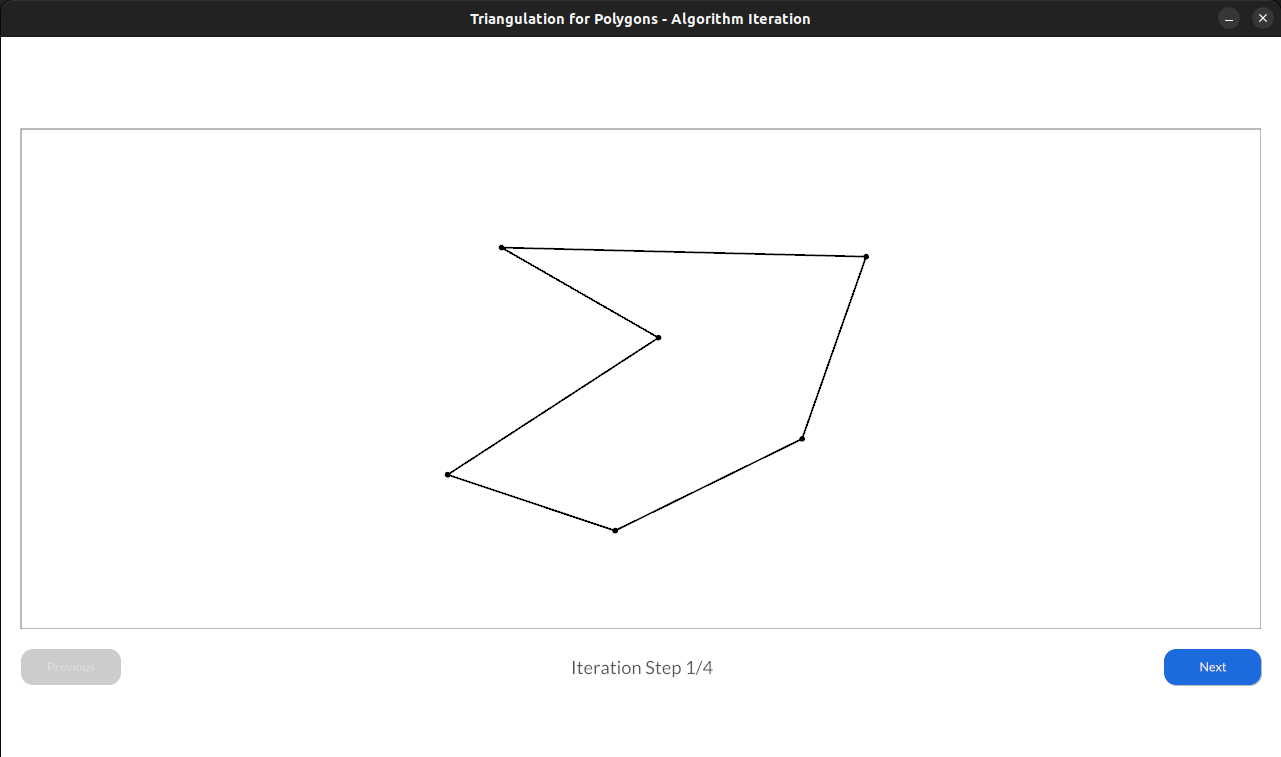
\includegraphics[width=1\textwidth]{bilder/iteration_final.png}
    \caption[Iterationsseite der Anwendung]{Iterationsseite der Anwendung als Bildschirmfoto}
\end{figure}

\subsubsection{Page - Result}

Die Ergebnisseite setzt sich aus zwei Anzeigefenstern mit zugehörigen Informationen zu den abgebildeten Triangulationen und einer Navigationsleiste zusammen.
Dabei ist das linke der beiden gleichgroßen Fenster das jenige, welches die durchlaufene Triangulation zeigt, die auf der Iterationsseite abgebiltet war. Darunter finden sich 
Informationen über das zerlegte Polygon. Namentlich der durchschnittliche Flächeninhalt der Dreiecke und deren durchschnittlicher kleinster Innenwinkel. Außedem wird die Anzahl an Ecken sowie Dreiecken angezeigt.

Das zweite Fenster soll in einer späteren Version eine Vergleichstriangulation, die \ac{dt}, zeigen. Ebenfalls sollen hier die Metadaten der Triangulation aufgezeigt werden.

Die Navigationsleiste besteht aus zwei Buttons. Auf der linken Seite befindet sich der \emph{Exit-Button}, welcher das Programm beendet. Damit der Nutzer weiterhin das Programm benutzen möchte, um weitere Triangulationen durchzuführen,
ist dieser Button im Sekundärstil gehalten.
Dagegen ist der andere Button auf der rechten Seite ein Primärbutton. Seine Beschriftung zeigt \emph{Return to Menu}. Wird er gedrückt, dann wird erneut das Menü aufgerufen. Im Zeichenfenster ist noch das zuvor eingegebene Polygon zu sehen.
Das hat den Zweck, dass der Nutzer mit dem selben Polygon aber anderen Einstellungen eine weitere Triangulation durchführen kann, welche eventuell ein besseres Ergebnis zeigt.
Eine denkbare Funktion wäre es, dass statt der \ac{dt} auf dem zweiten Anzeigefenster die vorangegangene Triangulation angezeigt wird, sofern sich das Polygon nicht verändert hat, welches zerlegt wird.

\begin{figure}[h]
    \centering
    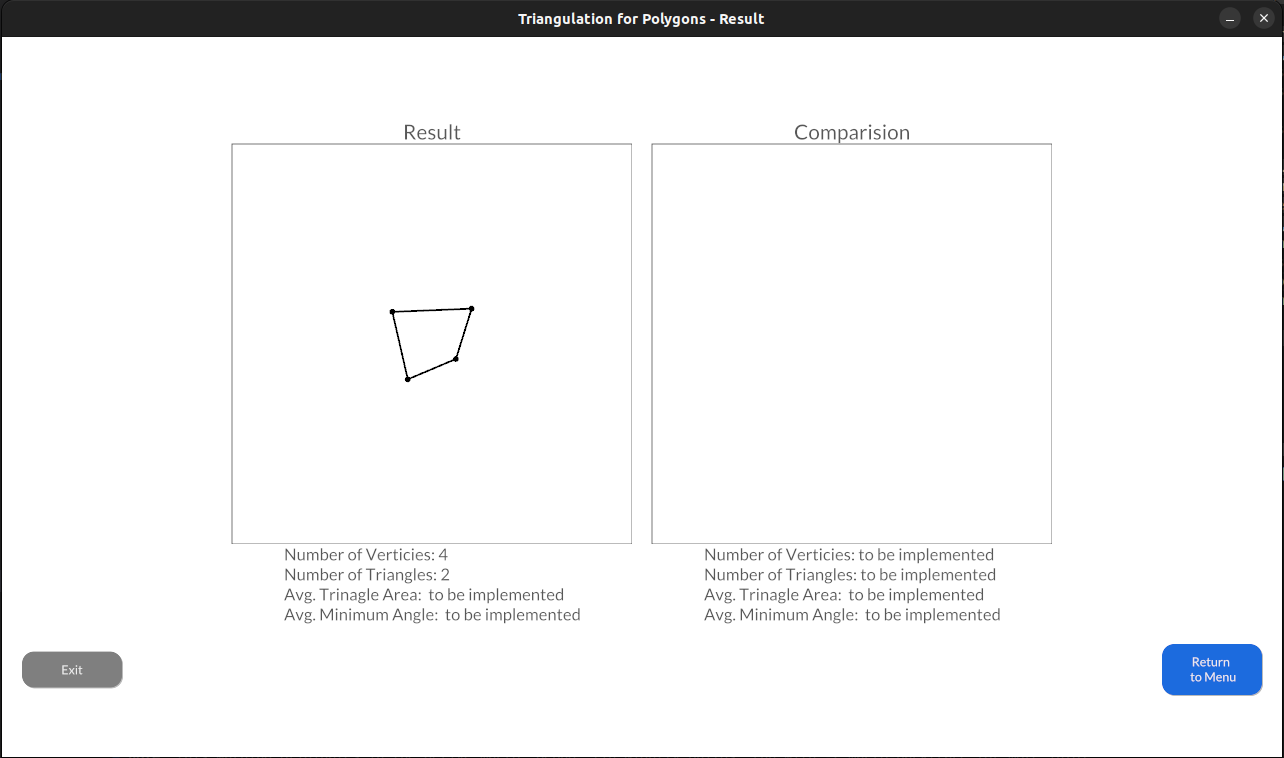
\includegraphics[width=1\textwidth]{bilder/result.png}
    \caption[Ergebnisseite der Anwendung]{Ergebnisseite der Anwendung als Bildschirmfoto}
\end{figure}


\subsubsection{Style und Dark Mode}
Ein großer Aspekt bei der Umsetzung von \ac{gui}s sind Farben. So haben bestimmte Farben für den Menschen bestimmte Bedeutungen - etwa Rot für Gefahr oder Ablehnung.
Dies nutzt man, um dem Benutzer bestimmte Botschaften zu übermitteln. So sind farblich hervorgehobene Buttons zum Beispiel wichtiger als graue. Hierfür müssen diese Farben festgelegt werden.
Das geschieht in der Datei \lstinline{style.rs} mittels der Implementierung von \lstinline{StyleSheets} für verschiedene Aufzählungstypen.
Dabei wird für jedes Interaktionselement wie Buttons, Radio Buttons aber auch für das Fenster selbst ein \lstinline{enum} erstellt, welcher alle verschiedenen Möglichkeiten für Stile des jeweiligen Elements 
umfasst. 

Hier soll einmal exemplarisch gezeigt werden, wie ein solches \lstinline{StyleSheet} für einen \lstinline{iced::container} aussieht. Dieser beinhaltet in jeder View-Funktion den Inhalt einer Seite 
und umfasst derher die Hintergrundfarbe \lstinline{backgroundcolor} und die Schriftfarbe \lstinline{text_color} des Anzeigefensters. 
Zuerst wird im Aufzählungstypen \lstinline{enum WindowStyle} festgelegt, wie viele unterschiedliche Stile ein solcher Container haben kann. 
Danach wird für jeden Stil pro Eigenschaft eine Farbe festgelegt. Alle Eigenschaften, welche dem festgelegten Standard der Iced-Bibliothek folgen sollen, werden mittels 
\lstinline{..Style::default()} abgebildet. So gibt es für Container in dieser Arbeit zwei Stile, wie für die meisten anderen Element auch. Die einzige Ausnahme bilden die Buttons, welche eine rot und grüne, 
sowie eine helle und eine dunkle Variante für Primär- und Sekundärbuttons besitzen. 
Alle anderen Elemente des \ac{gui} haben eine helle und eine dunkle Variante. Der sogenannte \emph{Dark Mode} ist eine weit verbreitete Option für vielerlei Anwendungsprogramme. Da er für einige Nutzer ein obligatorischer Modus ist,
ist er auch in dieser Arbeit implementiert. Er wird wie bereits erwähnt durch einen Toggler im Menü ein- oder ausgeschalten. Dadurch ändern sich alle Stile von der hellen auf die dunkele Variante oder umgekehrt. 
Standardmäßig ist der Dark Mode allerdings aus.

\begin{lstlisting}
    pub enum WindowStyle {
        Light,
        Dark
    }

    impl container::StyleSheet for WindowStyle {
        fn style(&self) -> container::Style {
            container::Style { 
                
                background:  Some(Background::Color(match self {
                    WindowStyle::Light => Color::WHITE,
                    WindowStyle::Dark => Color::from_rgb8(0x57, 0x57, 0x57),
                })),
                text_color: match self {
                    WindowStyle::Light => Some(Color::from_rgb8(0x57, 0x57, 0x57)),
                    WindowStyle::Dark => Some(Color::WHITE),
                },
                ..container::Style::default()
            }}}

\end{lstlisting}

Im nachfolgenden Bild ist der Dark Mode für das Menü als Beispiel angeführt.

\begin{figure}[h]
    \centering
    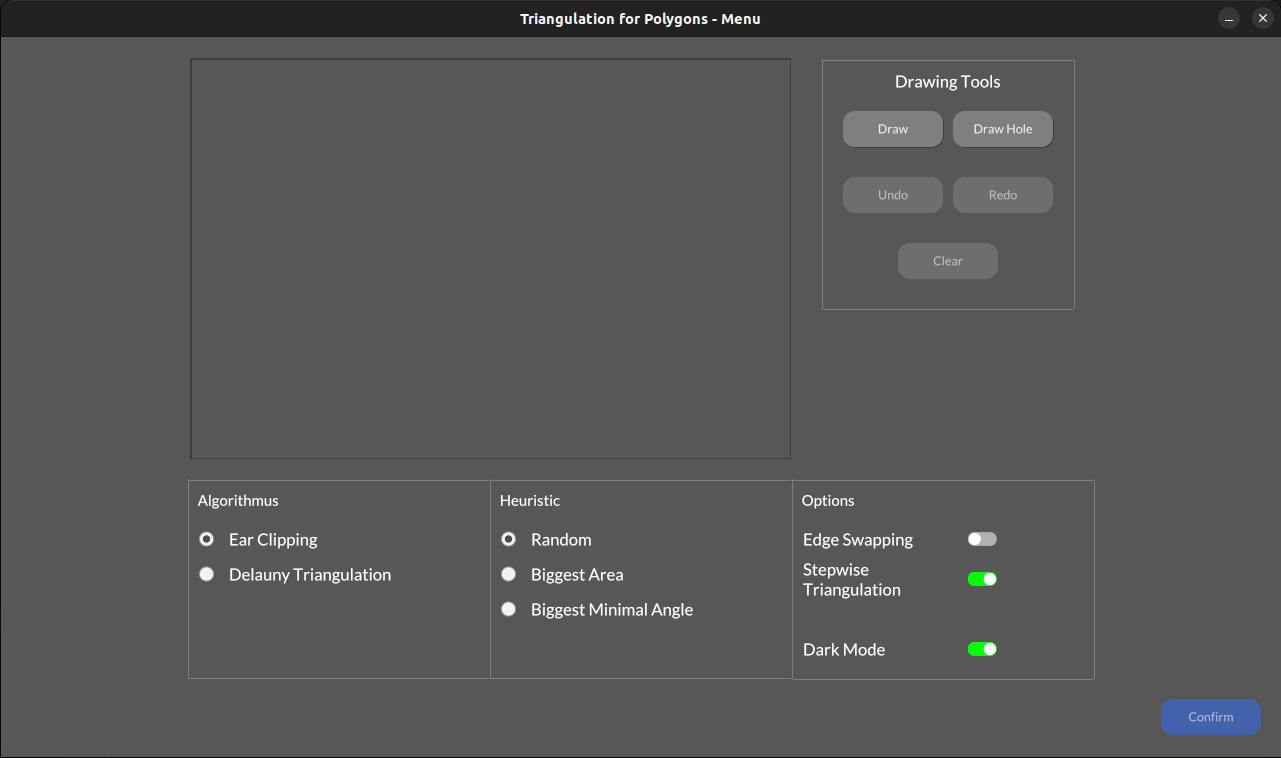
\includegraphics[width=1\textwidth]{bilder/darkmode.png}
    \caption[Menü im Dark Mode]{Das Menü der Anwendung dargestellt mit aktiviertem Dark Mode}
    
\end{figure}
%\subsubsection{Implementierung des Ear-Clipping-Algorithmus}

%\section{Auswertung}
\section{Ausblick und Zusammenfassung}
Wie bereits im Kapitl über die Praktische Implementierung angedeutet, gibt es einige Punkte, welche bis zum Zeitpunkt der Abgabe nicht umgesetzt wurden.
Diee seien hier als mögliche Erweiterungen und geplante Ergänzungen aufgeführt.

Allen Punkten voran steht die Implementierung der manuellen Auswahl von Dreiecken als Heuristik. Diese wurde Eingangs als Schwerpunkt genannt, welcher in dieser Arbeit zu erreihen sein soll. 
Aus zeitlichen Gründen, welche in der Auswertung genauer beleuchtet wurden, war es allerdings nicht möglich, diesen Punkt zu inkludieren. Geplant war es, dass die Nutzerauswahlen gespeichert, 
ausgewertet und in eine neue Heuristik überführt würden. Dies ist eine der größten möglichen Erweiterungen dieses Programms, da dadurch die Interaktivität dieser Software um ein Vielfaches 
ansteigen würde.

Auch ist es bisher noch nicht gelungen, die \ac{dt} als anwählbare Trinagulationsmethode einzubauen, geschweige, denn sie als Vergleich auf der Ergebnisseite 
anzubieten. Dies ist ein Punkt, welcher nicht im unmittelbaren Fokus der Arbeit lag, da der \ac{eca} explizit als Algorithmus angestrebt war.
Dennoch ist die Erweiterung des Programms, nicht nur um die \ac{dt} sondern auch um andere Triangulationsalgorithmen, durchaus denkbar und wünschenswert.

Bei Erweiterungen des Programms kommen auch weitere zusätzliche Heuristiken in Frage. Da auch ein Vergleich der Einflüsse von verschiedenen Heuristiken auf die Triangulationsqualität ein Ziel dieser 
Arbeit war, liegt es nur nahe, weitere solche Heuristiken einzubauen.

Auch an möglichen Optionen für die Triangulation und dem Erscheinungsbild der Anwendung besteht reichhaltiges Erweiterungspotential. Neben der in den theoretischen Grundlagen angesprochenen Methode des 
Edge Swappings sind auch andere Optionen wie beispielsweie ein unterer Grenzwert für den kleinsten Innenwinkel der Dreiecke denkbar. Liegt ein Innenwinkel unter desem Wert, könnte der Algorithmus dieses dann 
vorläufig ignorieren und erst dann auswählen, wenn keine besseren Optionen zur Verfügung stehen.

Aber auch an optischen Einstellungsmöglichkeiten könnte in Zukunft noch einiges optimiert und hinzugefügt werden. Neben dem bereits implementierten Dark Mode können auch andere Modi für bessere Lesbarkeit bei Farbenblindheit 
eingebaut werden. Auch eine Sprachauswahl ist denkbar, da die Software vorläufig nur in der englischen Sprache verfasst ist. Diese würde die Barrierefreiheit stark erhöhen, da es dann nicht mehr erforderlich wäre, des Englischen mächtig sein 
zu müssen.

Bei optischen Aspekten, welche die Nutzerfreundlichkeit erhöhen, kommen auch methaphorische Icons in den Sinn. An Stelle von Beschriftungen der Buttons könnten dann aussagekräftige Bilder stehen.
Ein Stift für die Zeichenoption, eine Mülltonne für das Löschen und ähnliches, was auch bereit in anderen Zeichenprogrammen gängig ist. Der Zugang des Nutzers würde dann steigen, sollte er zuvor einmal ein anderes Zeichenprogramm benutzt haben.
Es ist also noch einiges an Erweiterungen für die entworfene Software denkbar. \linebreak

Zusammenfassend gibt es also noch zu sagen, dass auf Grund zeitlicher Probleme nicht all die angedachten Features des Programms umgesetzt wurden. Das \ac{gui} allerdings ist ohne Fehler lauffähig.
Auch ist es möglich, eine Triangulation, wie angestrebt, durchzuführen und dies schrittweise. Damit ist einer der Hauptaspekte dieser Arbeit erfüllt. Die Anschaulichkeit einer Triangulation ist umgesetzt und kann beispielsweie
in der Lehre verwendet werden.
An anderer Stelle gibt es noch Verbesserungsbedarf. Es ist jedoch auch abzusehen, dass eine solche Software ständig erweiterbar ist und demnach keine wirkliche völlständige Implementierung erziehlt 
werden kann. Allein die Heuristiken für die Auswahl des nächsten Dreiecks sind nahezu endlos. 

\end{onehalfspacing}

\begin{thebibliography}{11}
    \raggedright
    \bibitem{digrev}
    \emph{Digitale Revolution} \break
    (\href{https://www.staatslexikon-online.de/Lexikon/Digitale_Revolution}{https://www.staatslexikon-online.de})

    \bibitem{polynet}
    \emph{Darstellung von Kurven und Flächen}, Christoph Dähne \break
    (\href{https://www.inf.tu-dresden.de/content/institutes/smt/cg/teaching/seminars/ProseminarSS08/cdaehne/ausarbeitung.pdf}{https://www.inf.tu-dresden.de})
    
    \bibitem{sliver}
    \emph{Geometrical Mesh Quality} \break
    (\href{https://www.iue.tuwien.ac.at/phd/fleischmann/node13.html#sec:geoqual}{https://www.iue.tuwien.ac.at})

    \bibitem{sliverdef}
    \emph{Sliver In: Computer Graphics Dictionary}, Stevens, R.T., 2002.
    
    \bibitem{earclipping2}
    \emph{Triangulation by Ear Clipping}, David Eberly \break 
    (\href{https://www.geometrictools.com/Documentation/TriangulationByEarClipping.pdf}{https://www.geometrictools.com})
    
    \bibitem{polytri}
    \emph{Polygon Triangulation}, Subhash Suri \break
    (\href{https://sites.cs.ucsb.edu/~suri/cs235/Triangulation.pdf}{https://sites.cs.ucsb.edu/~suri/cs235/Triangulation.pdf}) 
    
    \bibitem{paralleleca}
    \emph{Parallelized ear clipping for the triangulation and constrained Delaunay triangulation of polygons}, Günther Eder, Martin Held, Peter Palfrader \break
    (\href{https://www.sciencedirect.com/science/article/pii/S092577211830004X}{https://www.sciencedirect.com})

    \bibitem{improvedeca}
    \emph{Improved Algoritms For Ear-CLipping Triangulation}, Bartosz Kajak, 2005 \break
    (\href{https://digitalscholarship.unlv.edu/thesesdissertations/1319/}{https://digitalscholarship.unlv.edu/thesesdissertations/1319/})

    \bibitem{newAlg}
    \emph{A comparison of Ear Clipping and a new Polygon Triangulation Algorithm}, Ran Liu \break
    (\href{https://www.diva-portal.org/smash/get/diva2:330344/FULLTEXT02.pdf}{https://www.diva-portal.org/smash/get/diva2:330344/FULLTEXT02.pdf})

    \bibitem{polydef}
    \emph{Polygon, Definition} \break
    (\href{https://mathepedia.de/Polygone.html}{https://mathepedia.de/Polygone.html})
    
    \bibitem{regpoly}
    \emph{Regular Polygons. In: Michiel Hazewinkel (Hrsg.): Encyclopedia of Mathematics. Springer-Verlag und EMS Press, Berlin 2002}
    
    \bibitem{convex}
    \emph{Convex Polygon} \break
    (\href{https://www.mathopenref.com/polygonconvex.html}{https://www.mathopenref.com/polygonconvex.html})
    
    \bibitem{polytri3}
    \emph{Triangulation, Definition} \break
    (\href{https://encyclopediaofmath.org/wiki/Triangulation}{https://encyclopediaofmath.org/wiki/Triangulation})
    
    \bibitem{simplex}
    \emph{Simplex, Definition} \break
    (\href{https://encyclopediaofmath.org/wiki/Simplex}{https://encyclopediaofmath.org/wiki/Simplex})
    
    \bibitem{earclipping}
    \emph{Ear-clipping Based Algorithms of Generating High-quality Polygon Triangulation}, Gang Mei, John C.Tipper and Nengxiong Xu \break 
    (\href{https://arxiv.org/ftp/arxiv/papers/1212/1212.6038.pdf}{https://arxiv.org/ftp/arxiv/papers/1212/1212.6038.pdf})
    
    \bibitem{polytri2}
    \emph{Ear-Clipping Triangulierung} \break
    (\href{https://wiki.delphigl.com/index.php/Ear_Clipping_Triangulierung}{wiki.delphigl.com})
   
    \bibitem{jordan}
    \emph{Jordanscher Kurvensatz} \break
    (\href{https://de.wikipedia.org/wiki/Jordanscher_Kurvensatz}{https://de.wikipedia.org})

    \bibitem{cubecut}
    \emph{The smallest 8 cubes to cover a regular tetrahedron} \break
    (\href{https://math.stackexchange.com/questions/1423014/the-smallest-8-cubes-to-cover-a-regular-tetrahedron}{https://math.stackexchange.com/})
  
    \bibitem{twoears}
    \emph{Slicing an ear using prune-and-search In: Pattern Recognition Letters}, ElGindy, H., Everett, H., and Toussaint, G. T., (1993) S. 719-722

    \bibitem{meister}
    \emph{Polygons Have Ears In: Amer. Math. Monthly}, G.H. Meisters, Ausgabe 82, S. 648–651, 1975.

    \bibitem{tm}
    \emph{Turing-Maschinen In: Der Turing Omnibus}, A. K. Dewdney, S. 211-230, 1975.

    \bibitem{orourke}
    \emph{Computational Geometry In: C. Cambridge: Cambridge University Press}, O’Rourke, J., (1998). 

    \bibitem{goodrich}
    \emph{Triangulating a polygon in parallel In: Journal of Algorithms}, M. Goodrich, Ausgabe 10, S. 327-351, 1989. \break
    (\href{https://www.sciencedirect.com/science/article/pii/0196677489900321}{https://www.sciencedirect.com/})

    \bibitem{fist}
    \emph{FIST: Fast Industrial-Strength Triangulation of Polygons In: Algorithmica}, Held, M., Ausgabe 30, S. 563–596, 2001.
    ()\href{https://link.springer.com/article/10.1007/s00453-001-0028-4}{https://link.springer.com/article/10.1007/s00453-001-0028-4})
    
    \bibitem{dnc}
    \emph{Reentrant Polygon Clipping}, Sutherland, Ivan E. und Hodgman, Gary W., 1974. \break
    (\href{https://dl.acm.org/doi/abs/10.1145/360767.360802}{https://dl.acm.org/doi/abs/10.1145/360767.360802})
\end{thebibliography}

\end{document}